%!TEX encoding = UTF-8 Unicode
\documentclass[onecolumn,12pt]{book}\usepackage[]{graphicx}\usepackage[]{color}
%% maxwidth is the original width if it is less than linewidth
%% otherwise use linewidth (to make sure the graphics do not exceed the margin)
\makeatletter
\def\maxwidth{ %
  \ifdim\Gin@nat@width>\linewidth
    \linewidth
  \else
    \Gin@nat@width
  \fi
}
\makeatother

\definecolor{fgcolor}{rgb}{0.345, 0.345, 0.345}
\newcommand{\hlnum}[1]{\textcolor[rgb]{0.686,0.059,0.569}{#1}}%
\newcommand{\hlstr}[1]{\textcolor[rgb]{0.192,0.494,0.8}{#1}}%
\newcommand{\hlcom}[1]{\textcolor[rgb]{0.678,0.584,0.686}{\textit{#1}}}%
\newcommand{\hlopt}[1]{\textcolor[rgb]{0,0,0}{#1}}%
\newcommand{\hlstd}[1]{\textcolor[rgb]{0.345,0.345,0.345}{#1}}%
\newcommand{\hlkwa}[1]{\textcolor[rgb]{0.161,0.373,0.58}{\textbf{#1}}}%
\newcommand{\hlkwb}[1]{\textcolor[rgb]{0.69,0.353,0.396}{#1}}%
\newcommand{\hlkwc}[1]{\textcolor[rgb]{0.333,0.667,0.333}{#1}}%
\newcommand{\hlkwd}[1]{\textcolor[rgb]{0.737,0.353,0.396}{\textbf{#1}}}%

\usepackage{framed}
\makeatletter
\newenvironment{kframe}{%
 \def\at@end@of@kframe{}%
 \ifinner\ifhmode%
  \def\at@end@of@kframe{\end{minipage}}%
  \begin{minipage}{\columnwidth}%
 \fi\fi%
 \def\FrameCommand##1{\hskip\@totalleftmargin \hskip-\fboxsep
 \colorbox{shadecolor}{##1}\hskip-\fboxsep
     % There is no \\@totalrightmargin, so:
     \hskip-\linewidth \hskip-\@totalleftmargin \hskip\columnwidth}%
 \MakeFramed {\advance\hsize-\width
   \@totalleftmargin\z@ \linewidth\hsize
   \@setminipage}}%
 {\par\unskip\endMakeFramed%
 \at@end@of@kframe}
\makeatother

\definecolor{shadecolor}{rgb}{.97, .97, .97}
\definecolor{messagecolor}{rgb}{0, 0, 0}
\definecolor{warningcolor}{rgb}{1, 0, 1}
\definecolor{errorcolor}{rgb}{1, 0, 0}
\newenvironment{knitrout}{}{} % an empty environment to be redefined in TeX

\usepackage{alltt}
\usepackage[english,italian]{babel}
\usepackage[utf8]{inputenc}
\usepackage{inconsolata}
%\renewcommand*\familydefault{\ttdefault} %% Only if the base font of the document is to be typewriter style
\usepackage[T1]{fontenc}
\usepackage[buttonsize=1em]{animate}
\usepackage{a4wide,Sweave,url}
\usepackage{verbatim}
\usepackage{makeidx}
%\usepackage{babelbib}
\usepackage{float}
%\usepackage{fancyhdr}
\usepackage[T1]{fontenc}
%\usepackage[utf8]{inputenc}
\usepackage{framed}
\usepackage{lipsum}
\usepackage[]{color}
\usepackage{graphicx}
\usepackage{fancyvrb}
\usepackage{amsmath}
\usepackage{hyperref}
\newenvironment{question}{\item \textbf{Esercizio}\newline}{}
\newenvironment{solution}{\textbf{Soluzione}\newline}{}
\newenvironment{answerlist}{\renewcommand{\labelenumi}{(\alph{enumi})}\begin{enumerate}}{\end{enumerate}}
\definecolor{grigetto}{rgb}{0.9,0.9,0.9}
 
\DefineVerbatimEnvironment{Sinput}{Verbatim} {xleftmargin=2em} \DefineVerbatimEnvironment{Soutput}{Verbatim}{xleftmargin=2em} \DefineVerbatimEnvironment{Scode}{Verbatim}{xleftmargin=2em} \fvset{listparameters={\setlength{\topsep}{0pt}}} \renewenvironment{Schunk}{\small\vspace{\topsep}}{\vspace{\topsep}\normalsize}
%\usepackage{draftwatermark}
\usepackage{wrapfig}
\usepackage{listings}
\newcounter{fnotes}\setcounter{fnotes}{1}
\newcounter{Raction}\setcounter{Raction}{1}
\newcommand{\varia}[1]{\textsl{\textsf{#1}}}
\newcommand{\mytilde}{$\sim$}
\newcommand{\maurizio}[1]{\color{red}#1 \color{black}}
\newcommand{\federico}[1]{\color{green}#1 \color{black}}
 
\DefineVerbatimEnvironment{Soutput}{Verbatim}{xleftmargin=2em,   frame=single}
 \newenvironment{ese} [1]{\vskip10pt
 
 \markright{\today}
\colorbox{grigetto}{\parbox{\linewidth}{#1}}}
                          {
                
                          \medskip}
 \newcommand{\virgolette}{\selectlanguage{english}\texttt{"}\selectlanguage{italian}}
 \frontmatter\title{Matematica e Statistica con \textsf{R}}
\author{Federico Comoglio e  Maurizio Rinaldi}
\markright{\today}
\renewcommand{\chaptermark}[1]{%
 \markboth{\chaptername
 \ \thechapter.\ #1}{}}
\newcommand{\rst}{\textsf{RStudio}~}
\newcommand{\rpr}{\textsf{R}~}
\makeindex
\IfFileExists{upquote.sty}{\usepackage{upquote}}{}
\begin{document}
\setkeys{Gin}{width=0.7\textwidth}



\markright{\today}
\thispagestyle{empty}
\maketitle
\newpage
\thispagestyle{empty}
\tableofcontents
\newpage
\thispagestyle{empty}
 \mainmatter

 

 
 
\chapter{Statistica e probabilit\`a  con \textsf{R}}
Riprendiamo qui sinteticamente alcune definizioni.
\section{Lo spazio campionario}

Lo spazio campionario $\Omega$  (\emph{sample space}) è l'insieme di tutte le uscite possibili di un esperimento. Per esempio 
\begin{itemize}
\item Dado: lo spazio campionario consiste nelle uscite dei numeri da 1 a 6. \item Moneta: lo spazio campionario consiste di 2 possibili  uscite "esce testa", "esce croce"
\item Misure di lunghezza: lo spazio campionario è un intervallo del semiasse positivo della retta. 
Come si vede lo spazio campionario pu\`o essere dscreto o continuo. Potrebbe essere anche una combinazione dei due.
\end{itemize}
\section{Gli eventi}


 Un evento è un sottoinsieme dello spazio campionario. 
 Ad esempio
\begin{itemize}
\item Nel lancio di un dado l'uscita del 6 o l'uscita di un numero pari sono possibili eventi. 
\item Un evento semplice è un sottoinsieme di un elemento.
\end{itemize}


\subsubsection{Costruzione di eventi}

Siano A e  B degli eventi che possono risultare da un esperimento. A partire da questi eventi possiamo costruire dei nuovi eventi
\begin{itemize}
\item $A\cup B$ ($A$ oppure $B$, evento unione) indica il verificarsi di A o di B (o di ambedue).
\item $A \cap  B$  indica il verificarsi di A e di  B.
\item L'evento  $A^c$ (complemento di A, non A)   indica il non verificarsi dell'evento $A$.   
\end{itemize}
\begin{knitrout}
\definecolor{shadecolor}{rgb}{0.969, 0.969, 0.969}\color{fgcolor}
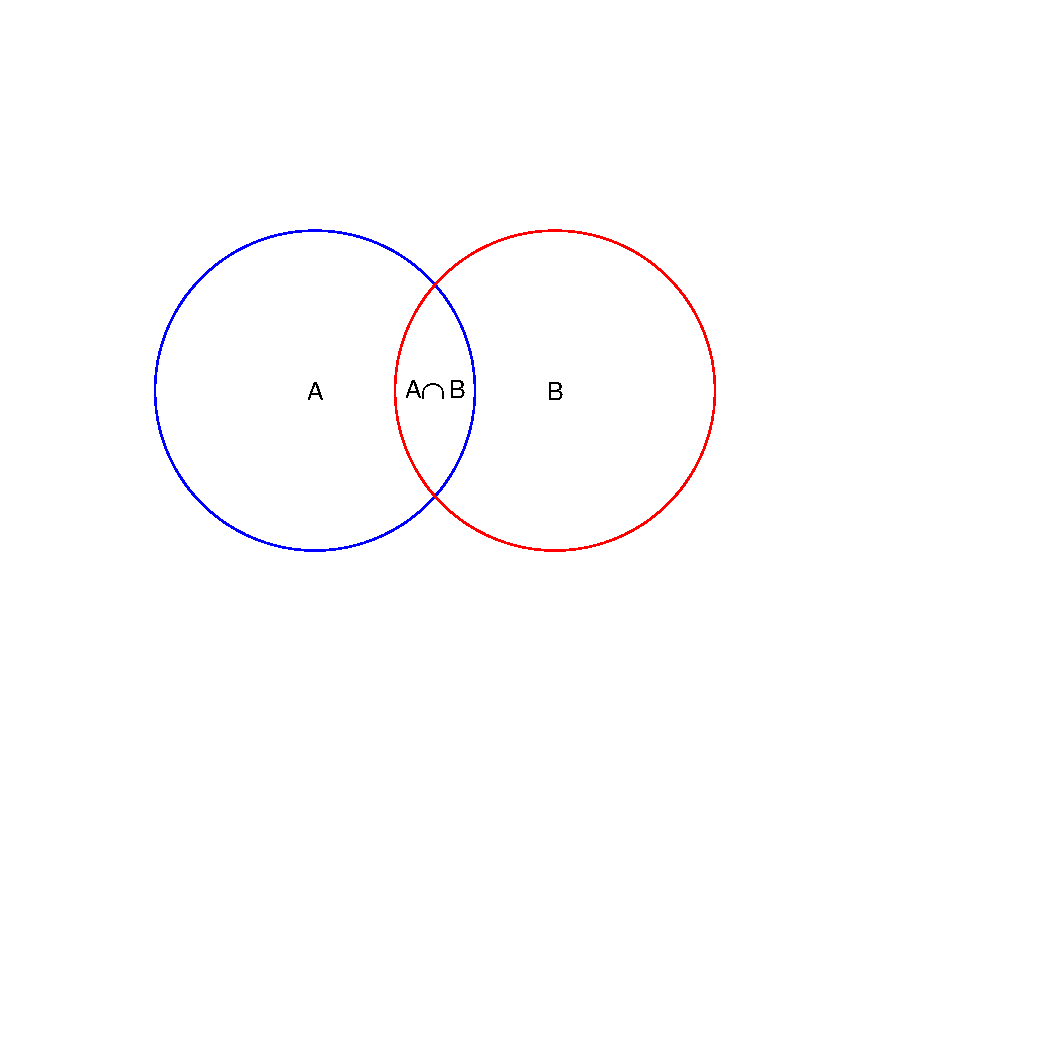
\includegraphics[width=\maxwidth]{figure/unnamed-chunk-3-1} 

\end{knitrout}


\section{La probabilità}

$P(A)$ indica la probabilità di un evento A. Questo è un numero nell'intervallo $[0,1]$ che possiamo associare a ciascun evento che soddisfa certe regole (assiomi).
Eventi certi corrispondono a probabilità uguale ad 1=100\%, eventi impossibili corrispondono a fiducia uguale a 0=0\%.

\subsubsection{ Assiomi}
\begin{enumerate}
\item qualunque sia l'evento $E$, $P(E)\geq 0$
\item $P(\Omega)=1$
\item  $P(E_1\cup E_2\cup\ldots \cup E_n)=P(E_1)+P(E_2)+\ldots +P(E_n)$ (anche per $n=\infty$) dove $E_i\cap E_j=\emptyset$
\end{enumerate}

Consideriamo ad esempio il lancio di un dado e sia
\begin{itemize}
\item  A = \texttt{esce pari}=$\{2,4,6\}$
\item  B = \texttt{esce un numero maggiore o uguale a 4}=$\{4,5,6\}$
\end{itemize}


Allora
$A\cup B=$\texttt{esce 2 o 4 o 5 o 6}=$\{2,4,5,6\}$

$A\cap B=$\texttt{esce 4 o 6}$=\{4,6\}$

$A^C=$ \texttt{esce un numero dispari}$=\{1,3,5\}$

$B^C=$\texttt{esce 1 o 2 o 3}$=\{1,2,3\}$
        
        
\subsection{Conseguenze}   


   
$A$ e $B$ sono \emph{incompatibili} se $A\cap B=\emptyset$.

\begin{knitrout}
\definecolor{shadecolor}{rgb}{0.969, 0.969, 0.969}\color{fgcolor}
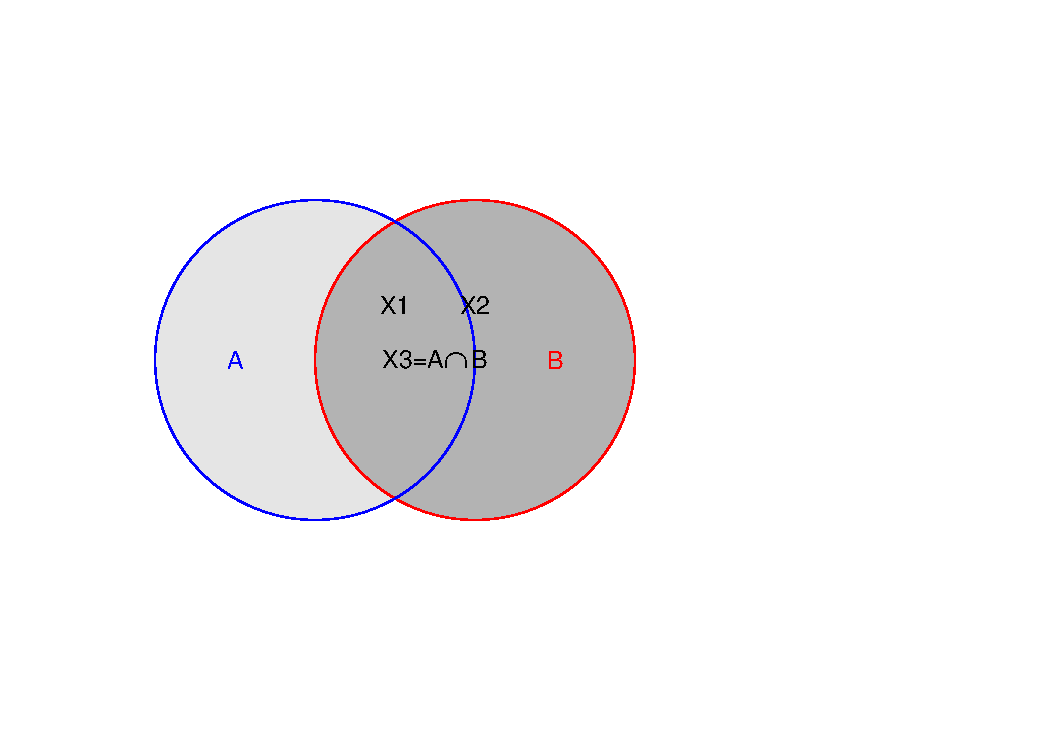
\includegraphics[width=\maxwidth]{figure/unnamed-chunk-4-1} 

\end{knitrout}

Abbiamo quindi
\[A=X_1\cup X_3, \quad B=X_2\cup X_3\]
da cui
\begin{align*} P(A)=&P(X_1)+P(X_3),\quad P(B)=P(X_3)+P(X_2)\\
 P(X_1)=&P(A)-P(X_3),\quad P(X_2)=P(B)-P(X_3)
 \end{align*}
\begin{align*} P(A\cup B)&=P(X_1\cup X_2\cup X_3)=P(X_1)+P(X_2)+P(X_3)=\\
&=P(A) +P(B)-P(X_3)=P(A) +P(B)-P(A\cap B)\end{align*}

e quindi 

$$P(A\cup B)=P(A) +P(B)-P(A\cap B)$$
ESEMPIO: Il 60\% degli studenti in questa classe è geniale mentre il   70\% ama lo sport; il 40\%, oltre ad essere geniale, ama lo sport. Determinare la probabilità che uno studente scelto a caso non sia geniale e non ami lo sport.


 
 

\section{Variabili aleatorie}
Una variabile aleatoria (\emph{random variabile}) \`e
 una variabile i cui valori sono soggetti a variazioni casuali. Quando i valori possibili di una variabile aleatoria  possono essere elencati parliamo di variabile aleatoria discreta. Quando i valori non possono essere elencati parliamo di variabile aleatoria continua.

\section{Variabili aleatorie discrete}
Le variabili aleatorie  discrete che  assumono un numero limitato di valori si dicono anche \emph{finite}.  I valori di una variabile aleatoria discreta possono essere numerici o nominali.
 Supponiamo di avere una variabile aleatoria che possa assumere un insieme di valori in  un \emph{alfabeto} assegnato costituito da lettere, parole o numeri. Per esempio un alfabeto pu\`o essere del tipo che segue
\begin{itemize}
\item{}(Femmina, Maschio)
\item{}(A,C,T,G)
\item{} (0,1)
\item{}(Ottimo, Buono, Discreto, Sufficiente, Insufficiente)
\item{} (Testa, Croce).
\item{} I numeri interi
\end{itemize}
Per caratterizzare completamente una variabile aleatoria discreta oltre ai valori che questa pu\`o  assumere occorre conoscere la probabilit\`a  di questi valori.
Per semplicit\`a considereremo variabili aleatorie finite.\\

 

La probabilità $P(A)$ di un evento A è il grado di fiducia  che lo sperimentatore pone nella realizzazione dell'evento (Jacob Bernoulli, 1654-1705) 

 
\subsection{Sistema completo di eventi}

Diciamo sistema completo

$$A_1, A_2,\ldots, A_N$$

un insieme di eventi relativi ad un certo esperimento tali che in ogni realizzazione dell'esperimento si verifichi uno e uno solo di essi. 

In generale sono un sistema completo di eventi si ha 

$$P(A_1)+P(A_2)+\ldots+ P(A_N) =1$$

\begin{itemize}
\item Lanciando una moneta possiamo prendere come sistema completo di eventi gli eventi $A_1$="esce testa" e $A_2$="esce croce" 
\item lanciando un dado   possiamo prendere come sistema completo di eventi le uscita $A_i$ dei numeri i da 1 a 6, ma anche gli eventi "esce pari", "esce dispari"
\end{itemize}
Se tutti gli eventi in un sistema completo di eventi sono equiprobabili possiamo facilmente ricavare la probabilità di ciascun evento.
 
$$P(A_1)+P(A_2)+\ldots+ P(A_N) =1=P(A_i)+P(A_i)+\ldots+ P(A_i)$$
$$P(A_i)=1/N$$
Nel caso del dado equo
$$P(\textrm{esce i}) = 1/6$$

\section{Lancio di 2 dadi}

Un  sistema completo di eventi i 36 eventi é 
$$A_{i,j}=\textrm{esce i sul dado verde e j sul dado rosso}$$ 
\begin{knitrout}
\definecolor{shadecolor}{rgb}{0.969, 0.969, 0.969}\color{fgcolor}\begin{kframe}
\begin{alltt}
\hlkwd{plot}\hlstd{(}\hlnum{0}\hlstd{,}\hlkwc{xlim}\hlstd{=}\hlkwd{c}\hlstd{(}\hlnum{0}\hlstd{,}\hlnum{6}\hlstd{),}\hlkwc{ylim}\hlstd{=}\hlkwd{c}\hlstd{(}\hlnum{0}\hlstd{,}\hlnum{12}\hlstd{),}\hlkwc{type}\hlstd{=}\hlstr{"n"}\hlstd{,}\hlkwc{axes}\hlstd{=F,}\hlkwc{xlab}\hlstd{=}\hlstr{""}\hlstd{,}\hlkwc{ylab}\hlstd{=}\hlstr{""}\hlstd{)}
\hlkwa{for} \hlstd{(i} \hlkwa{in} \hlnum{0}\hlopt{:}\hlnum{5}\hlstd{)}
\hlkwa{for} \hlstd{(j} \hlkwa{in} \hlnum{0}\hlopt{:}\hlnum{5}\hlstd{)}
\hlstd{\{}
\hlkwd{rect}\hlstd{(i,}\hlnum{2}\hlopt{*}\hlstd{j,}\hlnum{3}\hlopt{/}\hlnum{8}\hlopt{+}\hlstd{i,}\hlnum{2}\hlopt{*}\hlstd{j}\hlopt{+}\hlnum{1}\hlstd{,}\hlkwc{col}\hlstd{=}\hlstr{"red1"}\hlstd{)}
\hlkwd{rect}\hlstd{(}\hlnum{3}\hlopt{/}\hlnum{8}\hlopt{+}\hlstd{i,}\hlnum{2}\hlopt{*}\hlstd{j,}\hlnum{6}\hlopt{/}\hlnum{8}\hlopt{+}\hlstd{i,}\hlnum{1}\hlopt{+}\hlnum{2}\hlopt{*}\hlstd{j,}\hlkwc{col}\hlstd{=}\hlstr{"green"}\hlstd{)}
\hlkwd{text}\hlstd{(}\hlnum{3}\hlopt{/}\hlnum{16}\hlopt{+}\hlstd{i,}\hlnum{0.5}\hlopt{+}\hlnum{2}\hlopt{*}\hlstd{j,j}\hlopt{+}\hlnum{1}\hlstd{,}\hlkwc{cex}\hlstd{=}\hlnum{1}\hlstd{)}
\hlkwd{text}\hlstd{(i}\hlopt{+}\hlnum{9}\hlopt{/}\hlnum{16}\hlstd{,}\hlnum{0.5}\hlopt{+}\hlnum{2}\hlopt{*}\hlstd{j,i}\hlopt{+}\hlnum{1}\hlstd{,}\hlkwc{cex}\hlstd{=}\hlnum{1}\hlstd{)\}}
\end{alltt}
\end{kframe}
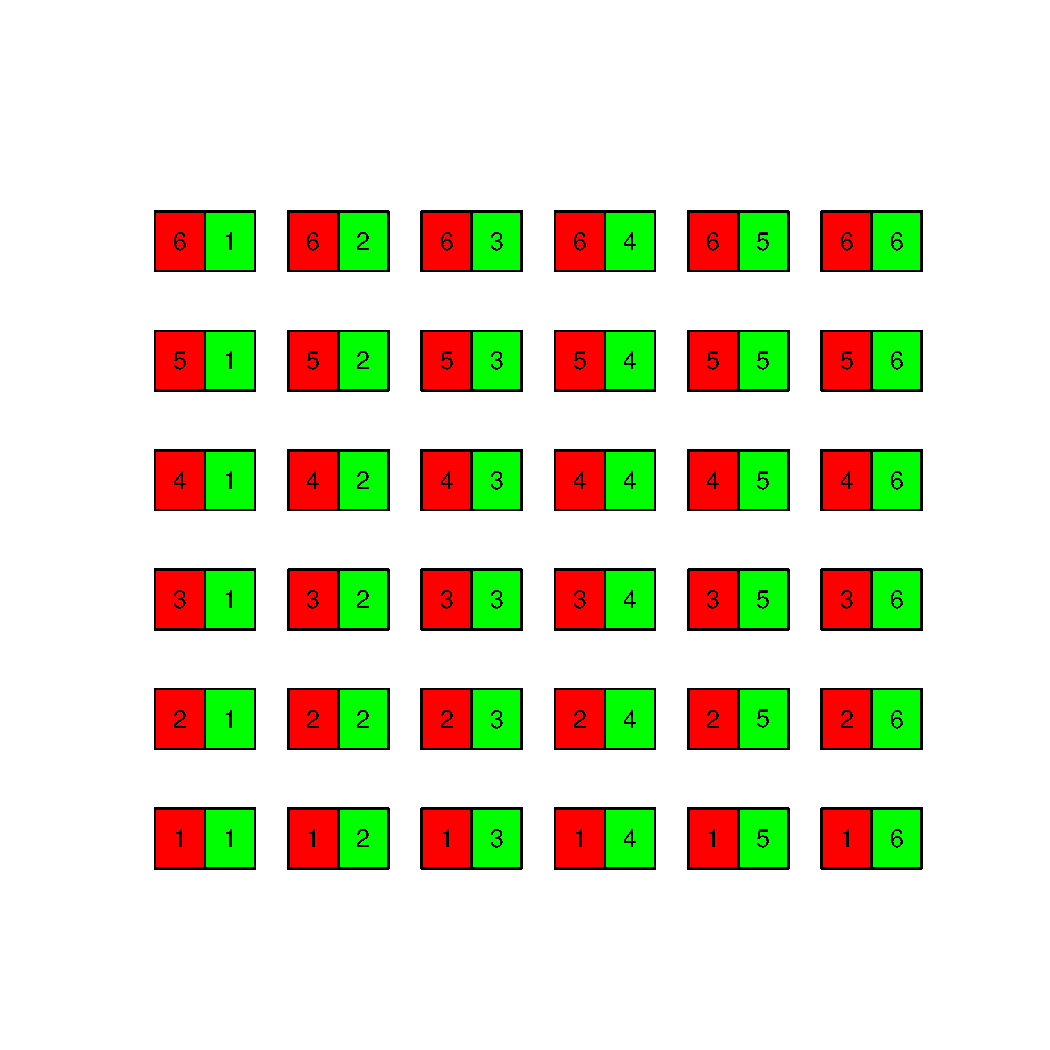
\includegraphics[width=\maxwidth]{figure/unnamed-chunk-5-1} 

\end{knitrout}
Se i dadi sono equi ogni evento  $A_{i,j}$ ha probabilità  1/36. 
Per esempio
$$P(\textrm{la somma fa 8})$$
 
 
\section{Probabilità condizionata}

La notazione 

$$P(A\mid B)$$

indica la probabilità  dell'evento $A$ condizionata al verificarsi dell'evento $B$.
In altre parole quale é la probabilità che si verifichi $A$ quando anche $B$ é verificato. 
\begin{knitrout}
\definecolor{shadecolor}{rgb}{0.969, 0.969, 0.969}\color{fgcolor}\begin{kframe}
\begin{alltt}
\hlkwd{set.seed}\hlstd{(}\hlnum{2000}\hlstd{)}
\hlkwd{par}\hlstd{(}\hlkwc{mai}\hlstd{=}\hlkwd{c}\hlstd{(}\hlnum{0}\hlstd{,}\hlnum{0}\hlstd{,}\hlnum{0}\hlstd{,}\hlnum{0}\hlstd{))}
\hlkwd{par}\hlstd{(}\hlkwc{mgp}\hlstd{=}\hlkwd{c}\hlstd{(}\hlnum{0}\hlstd{,}\hlnum{0}\hlstd{,}\hlnum{0}\hlstd{))}
\hlstd{n}\hlkwb{=}\hlnum{30}
\hlkwd{library}\hlstd{(plotrix)}
\hlkwd{plot}\hlstd{(}\hlnum{0}\hlstd{,}\hlnum{0}\hlstd{,}\hlkwc{xlim}\hlstd{=}\hlkwd{c}\hlstd{(}\hlopt{-}\hlnum{1}\hlstd{,}\hlnum{11}\hlstd{),}\hlkwc{ylim}\hlstd{=}\hlkwd{c}\hlstd{(}\hlopt{-}\hlnum{1}\hlstd{,}\hlnum{11}\hlstd{),}\hlkwc{type}\hlstd{=}\hlstr{"n"}\hlstd{,}\hlkwc{xlab}\hlstd{=}\hlstr{""}\hlstd{,}\hlkwc{ylab}\hlstd{=}\hlstr{""}\hlstd{,}\hlkwc{asp}\hlstd{=}\hlnum{1}\hlstd{,}\hlkwc{axes}\hlstd{=F,}
     \hlstd{)}
\hlkwd{rect}\hlstd{(}\hlnum{0}\hlstd{,}\hlnum{0}\hlstd{,}\hlnum{10}\hlstd{,}\hlnum{10}\hlstd{,}\hlkwc{border}\hlstd{=}\hlstr{"green"}\hlstd{,}\hlkwc{lwd}\hlstd{=}\hlnum{2}\hlstd{)}
\hlstd{centro1}\hlkwb{=}\hlkwd{c}\hlstd{(}\hlnum{4}\hlstd{,}\hlnum{4}\hlstd{)}
\hlstd{centro2}\hlkwb{=}\hlkwd{c}\hlstd{(}\hlnum{5}\hlstd{,}\hlnum{5}\hlstd{)}
\hlkwd{draw.circle}\hlstd{(centro1[}\hlnum{1}\hlstd{],centro1[}\hlnum{2}\hlstd{],}\hlnum{2}\hlstd{,}\hlkwc{border}\hlstd{=}\hlstr{"blue"}\hlstd{)}
\hlkwd{draw.circle}\hlstd{(centro2[}\hlnum{1}\hlstd{],centro2[}\hlnum{2}\hlstd{],}\hlnum{2}\hlstd{,}\hlkwc{border}\hlstd{=}\hlstr{"red"}\hlstd{,}\hlkwc{lwd}\hlstd{=}\hlnum{3}\hlstd{,}\hlkwc{col}\hlstd{=}\hlstr{"light green"}\hlstd{)}
\hlstd{punti}\hlkwb{=}\hlkwd{cbind}\hlstd{(}\hlkwd{runif}\hlstd{(n,}\hlnum{0}\hlstd{,}\hlnum{10}\hlstd{),}\hlkwd{runif}\hlstd{(n,}\hlnum{0}\hlstd{,}\hlnum{10}\hlstd{))}
\hlkwd{points}\hlstd{(punti,}\hlkwc{cex}\hlstd{=}\hlnum{0.8}\hlstd{,}\hlkwc{pch}\hlstd{=}\hlnum{19}\hlstd{)}
\hlkwd{draw.circle}\hlstd{(}\hlnum{4}\hlstd{,}\hlnum{4}\hlstd{,}\hlnum{2}\hlstd{,}\hlkwc{lwd}\hlstd{=}\hlnum{3}\hlstd{,}\hlkwc{border}\hlstd{=}\hlstr{"blue"}\hlstd{)}
\hlkwd{text}\hlstd{(}\hlnum{3}\hlstd{,}\hlnum{3}\hlstd{,}\hlstr{"A"}\hlstd{,}\hlkwc{col}\hlstd{=}\hlstr{"blue"}\hlstd{)}
\hlkwd{text}\hlstd{(}\hlnum{6}\hlstd{,}\hlnum{6}\hlstd{,}\hlstr{"B"}\hlstd{)}
\hlkwd{text}\hlstd{(}\hlnum{4}\hlstd{,}\hlnum{4}\hlstd{,}\hlkwd{expression}\hlstd{(}\hlkwd{paste}\hlstd{(}\hlstr{"A"}\hlstd{,}\hlkwd{intersect}\hlstd{(}\hlstr{"B"}\hlstd{))))}
\hlkwd{title}\hlstd{(}\hlstr{"n=30"}\hlstd{,}\hlkwc{line}\hlstd{=}\hlopt{-}\hlnum{2}\hlstd{)}
\end{alltt}
\end{kframe}
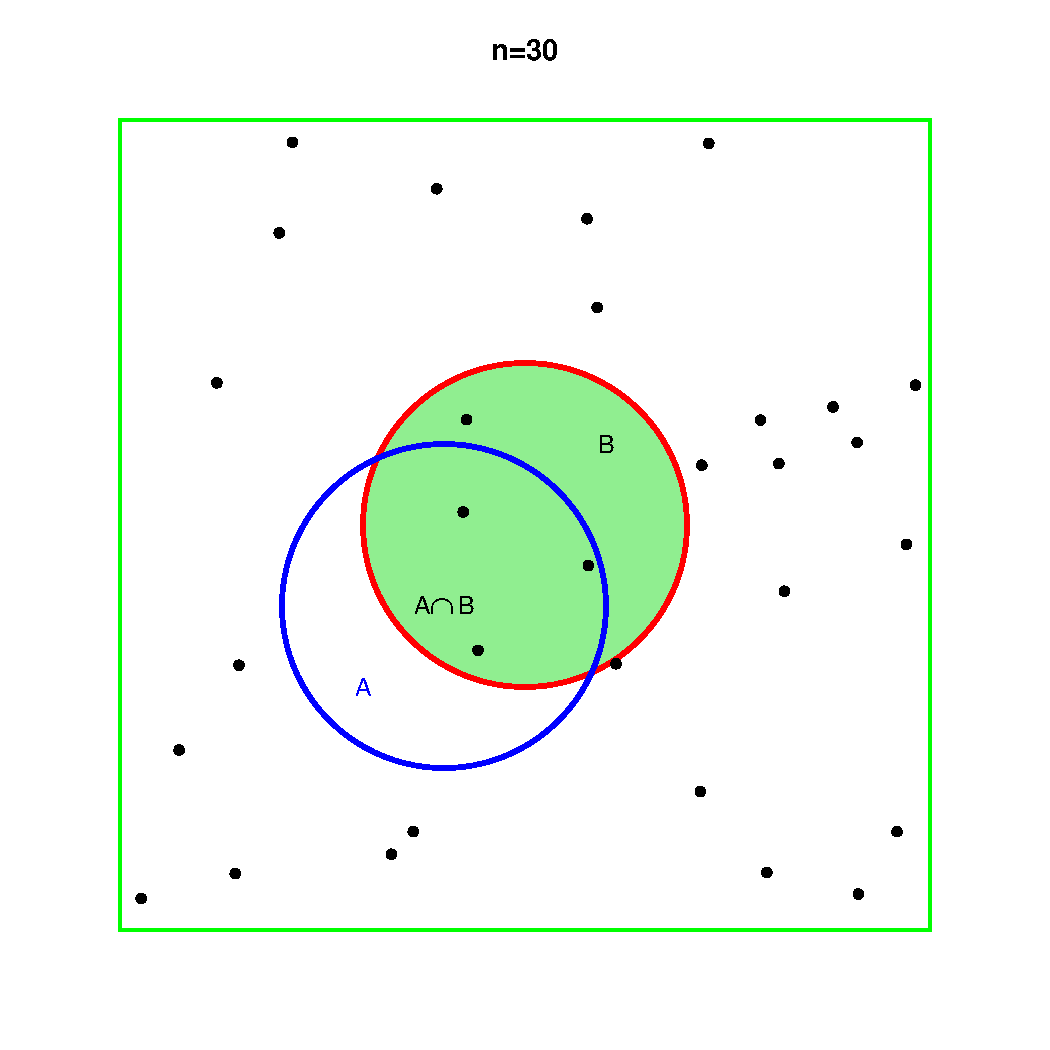
\includegraphics[width=\maxwidth]{figure/unnamed-chunk-6-1} 

\end{knitrout}


 
\begin{knitrout}
\definecolor{shadecolor}{rgb}{0.969, 0.969, 0.969}\color{fgcolor}\begin{kframe}
\begin{alltt}
\hlkwd{library}\hlstd{(MASS)}
\end{alltt}


{\ttfamily\noindent\itshape\color{messagecolor}{\#\# \\\#\# Attaching package: 'MASS'}}

{\ttfamily\noindent\itshape\color{messagecolor}{\#\# The following object is masked from 'package:EsamiR':\\\#\# \\\#\#\ \ \ \  crabs}}\begin{alltt}
\hlstd{a}\hlkwb{=}\hlkwd{length}\hlstd{(}\hlkwd{which}\hlstd{(}\hlkwd{rowSums}\hlstd{((punti}\hlopt{-}\hlstd{centro1)}\hlopt{^}\hlnum{2}\hlstd{)}\hlopt{<}\hlnum{4}\hlstd{))}
\hlstd{b}\hlkwb{=}\hlkwd{length}\hlstd{(}\hlkwd{which}\hlstd{(}\hlkwd{rowSums}\hlstd{((punti}\hlopt{-}\hlstd{centro2)}\hlopt{^}\hlnum{2}\hlstd{)}\hlopt{<}\hlnum{4}\hlstd{))}
\hlstd{acapb}\hlkwb{=}\hlkwd{length}\hlstd{(}\hlkwd{which}\hlstd{(}\hlkwd{rowSums}\hlstd{((punti}\hlopt{-}\hlstd{centro1)}\hlopt{^}\hlnum{2}\hlstd{)}\hlopt{<}\hlnum{4} \hlopt{&} \hlkwd{rowSums}\hlstd{((punti}\hlopt{-}\hlstd{centro2)}\hlopt{^}\hlnum{2}\hlstd{)}\hlopt{<}\hlnum{4}\hlstd{))}
\end{alltt}
\end{kframe}
\end{knitrout}

$$P(A| B)=\frac{n_{A\cap B}}{n_{B}}=\frac{n_{A\cap B}/n}{n_{B}/n}=\frac{P({A\cap B})}{P(B)}=3/4$$

Quindi 
$$P(A| B)=\frac{P({A\cap B})}{P(B)}\quad (\hbox{se } B\neq \emptyset)$$

\section{Esempio  1}

\begin{knitrout}
\definecolor{shadecolor}{rgb}{0.969, 0.969, 0.969}\color{fgcolor}\begin{kframe}
\begin{alltt}
\hlkwd{set.seed}\hlstd{(}\hlnum{10}\hlstd{)}
\hlkwd{load}\hlstd{(}\hlstr{"../cards.Rdata"}\hlstd{)}
\hlkwd{library}\hlstd{(XML)}
\hlkwd{library}\hlstd{(grid)}
\hlkwd{library}\hlstd{(grImport)}
\hlstd{mazzo}\hlkwb{=}\hlkwd{names}\hlstd{(cards)[}\hlnum{1}\hlopt{:}\hlnum{40}\hlstd{]}
\hlkwd{sample}\hlstd{(mazzo,}\hlnum{10}\hlstd{)}\hlkwb{->}\hlstd{estratte}
\hlkwd{plot}\hlstd{(}\hlkwd{numeric}\hlstd{(}\hlnum{0}\hlstd{),}\hlkwc{xlim}\hlstd{=}\hlkwd{c}\hlstd{(}\hlnum{0}\hlstd{,}\hlnum{7}\hlstd{),}\hlkwc{ylim}\hlstd{=}\hlkwd{c}\hlstd{(}\hlnum{0}\hlstd{,}\hlnum{2}\hlstd{),}\hlkwc{xlab}\hlstd{=}\hlstr{""}\hlstd{,}\hlkwc{ylab}\hlstd{=}\hlstr{""}\hlstd{,}\hlkwc{axes}\hlstd{=F)}
\hlkwa{for} \hlstd{(i} \hlkwa{in} \hlnum{1}\hlopt{:}\hlnum{5}\hlstd{)}
\hlkwd{picture}\hlstd{(cards[[estratte[i]]],i}\hlopt{*}\hlnum{1.2}\hlstd{,}\hlnum{1}\hlstd{,(i}\hlopt{+}\hlnum{1}\hlstd{)}\hlopt{*}\hlnum{1.2}\hlstd{,}\hlnum{2}\hlstd{)}
\hlkwa{for} \hlstd{(i} \hlkwa{in} \hlnum{1}\hlopt{:}\hlnum{5}\hlstd{)}
\hlkwd{picture}\hlstd{(cards[[estratte[i}\hlopt{+}\hlnum{5}\hlstd{]]],i}\hlopt{*}\hlnum{1.2}\hlstd{,}\hlnum{0}\hlstd{,(i}\hlopt{+}\hlnum{1}\hlstd{)}\hlopt{*}\hlnum{1.2}\hlstd{,}\hlnum{1}\hlstd{)}
\end{alltt}
\end{kframe}
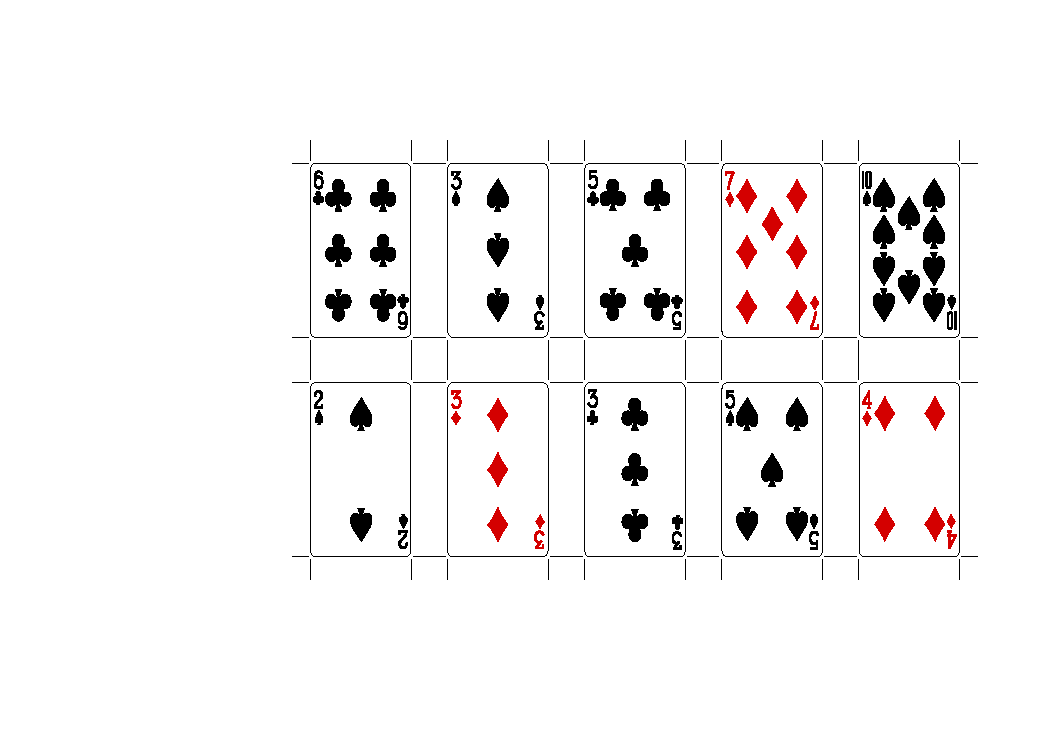
\includegraphics[width=\maxwidth]{figure/unnamed-chunk-8-1} 

\end{knitrout}

\begin{knitrout}
\definecolor{shadecolor}{rgb}{0.969, 0.969, 0.969}\color{fgcolor}\begin{kframe}
\begin{alltt}
\hlkwd{strsplit}\hlstd{(estratte,}\hlkwc{split}\hlstd{=}\hlstr{"[.]"}\hlstd{)}\hlkwb{->}\hlstd{temp}
\hlkwd{as.numeric}\hlstd{(}\hlkwd{sapply}\hlstd{(temp,}\hlstr{"["}\hlstd{,}\hlnum{2}\hlstd{))}\hlkwb{->}\hlstd{valore}
\hlstd{pari}\hlkwb{=}\hlkwd{which}\hlstd{(valore}\hlopt\hlnum{2}\hlopt{==}\hlnum{0}\hlstd{)}
\hlstd{rosse}\hlkwb{=}\hlkwd{which}\hlstd{(}\hlkwd{sapply}\hlstd{(temp,}\hlstr{"["}\hlstd{,}\hlnum{1}\hlstd{)}\hlopt{==}\hlstr{"C"}\hlopt{|}\hlkwd{sapply}\hlstd{(temp,}\hlstr{"["}\hlstd{,}\hlnum{1}\hlstd{)}\hlopt{==}\hlstr{"Q"}\hlstd{)}
\hlkwd{library}\hlstd{(MASS)}
\end{alltt}
\end{kframe}
\end{knitrout}

\(P(\textrm{Rosso})\)= 3/10

\(P(\textrm{Pari})\)=  4/10
 
\(P(\textrm{Rosso}\cap \textrm{Pari})\)

> - 1/10

\(P(\textrm{Rosso}\mid \textrm{Pari}) \)

> - 1/4

\(P(\textrm{Pari}\mid \textrm{Rosso}) \)

> - 1/3

\(P(\textrm{Pari}\cup\textrm{Rossa})\)

6/10

\section{Esempio 2}

\begin{knitrout}
\definecolor{shadecolor}{rgb}{0.969, 0.969, 0.969}\color{fgcolor}\begin{kframe}
\begin{alltt}
\hlstd{n}\hlkwb{=}\hlnum{7}
\hlkwd{sample}\hlstd{(mazzo,}\hlnum{2}\hlopt{*}\hlstd{n)}\hlkwb{->}\hlstd{estratte}
\hlkwd{plot}\hlstd{(}\hlkwd{numeric}\hlstd{(}\hlnum{0}\hlstd{),}\hlkwc{xlim}\hlstd{=}\hlkwd{c}\hlstd{(}\hlnum{0}\hlstd{,}\hlnum{1.4}\hlopt{*}\hlstd{n),}\hlkwc{ylim}\hlstd{=}\hlkwd{c}\hlstd{(}\hlnum{0}\hlstd{,}\hlnum{2}\hlopt{*}\hlnum{5}\hlopt{/}\hlstd{n),}\hlkwc{xlab}\hlstd{=}\hlstr{""}\hlstd{,}\hlkwc{ylab}\hlstd{=}\hlstr{""}\hlstd{,}\hlkwc{axes}\hlstd{=F)}
\hlkwa{for} \hlstd{(i} \hlkwa{in} \hlnum{1}\hlopt{:}\hlstd{n)}
\hlkwd{picture}\hlstd{(cards[[estratte[i]]],i}\hlopt{*}\hlnum{1.2}\hlstd{,}\hlnum{5}\hlopt{/}\hlstd{n,(i}\hlopt{+}\hlnum{1}\hlstd{)}\hlopt{*}\hlnum{1.2}\hlstd{,}\hlnum{2}\hlopt{*}\hlnum{5}\hlopt{/}\hlstd{n)}
\hlkwa{for} \hlstd{(i} \hlkwa{in} \hlnum{1}\hlopt{:}\hlstd{n)}
\hlkwd{picture}\hlstd{(cards[[estratte[i}\hlopt{+}\hlstd{n]]],i}\hlopt{*}\hlnum{1.2}\hlstd{,}\hlnum{0}\hlstd{,(i}\hlopt{+}\hlnum{1}\hlstd{)}\hlopt{*}\hlnum{1.2}\hlstd{,}\hlnum{1}\hlopt{*}\hlnum{5}\hlopt{/}\hlstd{n)}
\end{alltt}
\end{kframe}
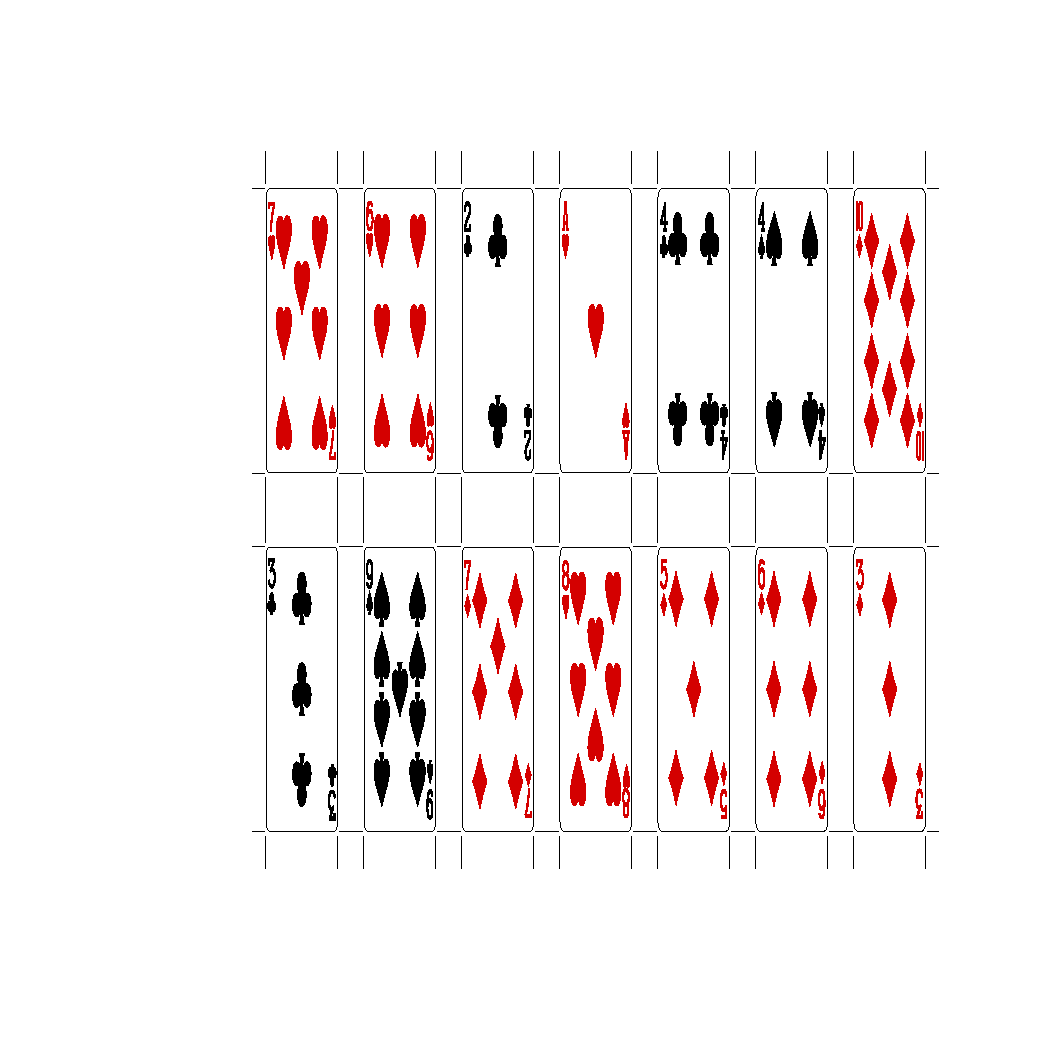
\includegraphics[width=\maxwidth]{figure/unnamed-chunk-10-1} 

\end{knitrout}

\begin{knitrout}
\definecolor{shadecolor}{rgb}{0.969, 0.969, 0.969}\color{fgcolor}\begin{kframe}
\begin{alltt}
\hlkwd{strsplit}\hlstd{(estratte,}\hlkwc{split}\hlstd{=}\hlstr{"[.]"}\hlstd{)}\hlkwb{->}\hlstd{temp}
\hlkwd{as.numeric}\hlstd{(}\hlkwd{sapply}\hlstd{(temp,}\hlstr{"["}\hlstd{,}\hlnum{2}\hlstd{))}\hlkwb{->}\hlstd{valore}
\hlstd{pari}\hlkwb{=}\hlkwd{which}\hlstd{(valore}\hlopt\hlnum{2}\hlopt{==}\hlnum{0}\hlstd{)}
\hlstd{rosse}\hlkwb{=}\hlkwd{which}\hlstd{(}\hlkwd{sapply}\hlstd{(temp,}\hlstr{"["}\hlstd{,}\hlnum{1}\hlstd{)}\hlopt{==}\hlstr{"C"}\hlopt{|}\hlkwd{sapply}\hlstd{(temp,}\hlstr{"["}\hlstd{,}\hlnum{1}\hlstd{)}\hlopt{==}\hlstr{"Q"}\hlstd{)}
\hlkwd{library}\hlstd{(MASS)}
\end{alltt}
\end{kframe}
\end{knitrout}

\(P(\textrm{Rosso})\)

> -  9/14

\(P(\textrm{Pari})\)

> -  7/14
 
\(P(\textrm{Rosso}\cap \textrm{Pari})\)

> - 4/14

\(P(\textrm{Rosso}\mid \textrm{Pari}) \)

> - 4/7

\(P(\textrm{Pari}\mid \textrm{Rosso}) \)

> - 4/9

\(P(\textrm{Pari}\cup\textrm{Rossa})\)

> -  12/14

 

Consideriamo una popolazione P di $N=10^6$ individui uomini o donne $(M/W)$ che possono essere mancini o destrorsi $(L/R)$. Sia

$$WL =\textrm{Donne Mancine}=60000$$
$$L=\textrm{Mancini totali}= 110000$$
$$W=\textrm{Donne}= 650000$$

\begin{knitrout}
\definecolor{shadecolor}{rgb}{0.969, 0.969, 0.969}\color{fgcolor}\begin{kframe}
\begin{alltt}
\hlkwd{options}\hlstd{(}\hlkwc{scipen}\hlstd{=}\hlnum{999}\hlstd{)}
\hlstd{mancini}\hlkwb{=}\hlkwd{data.frame}\hlstd{(}\hlkwd{c}\hlstd{(}\hlnum{60000}\hlstd{,}\hlstr{"-"}\hlstd{,}\hlnum{110000}\hlstd{),}\hlkwd{rep}\hlstd{(}\hlstr{"-"}\hlstd{,}\hlnum{3}\hlstd{),}\hlkwd{c}\hlstd{(}\hlnum{650000}\hlstd{,}\hlstr{"-"}\hlstd{,} \hlnum{1000000}\hlstd{))}
\hlkwd{colnames}\hlstd{(mancini)}\hlkwb{=}\hlkwd{c}\hlstd{(}  \hlstr{"L"}\hlstd{,} \hlstr{"R"}\hlstd{,} \hlstr{"Totali"}\hlstd{)}
\hlkwd{rownames}\hlstd{(mancini)}\hlkwb{=}\hlkwd{c}\hlstd{(}\hlstr{"W"}\hlstd{,} \hlstr{"M"}\hlstd{,} \hlstr{"Totali"}\hlstd{)}
 \hlkwd{library}\hlstd{(knitr)}
\hlkwd{kable}\hlstd{(mancini)}
\end{alltt}
\end{kframe}
\begin{tabular}{l|l|l|l}
\hline
  & L & R & Totali\\
\hline
W & 60000 & - & 650000\\
\hline
M & - & - & -\\
\hline
Totali & 110000 & - & 1000000\\
\hline
\end{tabular}


\end{knitrout}

Completando la tabella


\begin{knitrout}
\definecolor{shadecolor}{rgb}{0.969, 0.969, 0.969}\color{fgcolor}\begin{kframe}
\begin{alltt}
\hlstd{mancini}\hlkwb{=}\hlkwd{matrix}\hlstd{(}\hlkwd{c}\hlstd{(}\hlnum{60000}\hlstd{,}\hlnum{590000}\hlstd{,}\hlnum{650000}\hlstd{,}\hlnum{50000}\hlstd{,} \hlnum{300000}\hlstd{,} \hlnum{350000}\hlstd{,}  \hlnum{110000}\hlstd{,} \hlnum{890000}\hlstd{,} \hlnum{1000000}\hlstd{),}\hlkwc{nrow}\hlstd{=}\hlnum{3}\hlstd{,}\hlkwc{byrow}\hlstd{=T)}
\hlkwd{colnames}\hlstd{(mancini)}\hlkwb{=}\hlkwd{c}\hlstd{(}  \hlstr{"L"}\hlstd{,} \hlstr{"R"}\hlstd{,} \hlstr{"Totali"}\hlstd{)}
\hlkwd{rownames}\hlstd{(mancini)}\hlkwb{=}\hlkwd{c}\hlstd{(}\hlstr{"W"}\hlstd{,} \hlstr{"M"}\hlstd{,} \hlstr{"Totali"}\hlstd{)}
 \hlkwd{library}\hlstd{(knitr)}
\hlkwd{kable}\hlstd{(mancini)}
\end{alltt}
\end{kframe}
\begin{tabular}{l|r|r|r}
\hline
  & L & R & Totali\\
\hline
W & 60000 & 590000 & 650000\\
\hline
M & 50000 & 300000 & 350000\\
\hline
Totali & 110000 & 890000 & 1000000\\
\hline
\end{tabular}


\end{knitrout}


Per calcolare $P(L \mid  W)$  occorre determinare la probabilità di essere mancini se si é donne. In altre parole la popolazione é quella delle donne e all'interno di quello determiniamo  la probabilità di essere mancini:


$$P(L) = 110000/1000000=0.11$$
$$P(W)= 650000/1000000=0.65$$
$$P(L \cap  W) = 60000/1000000$$

$$P (L \mid W)=(\# \textrm{Donne mancine})/(\# \textrm{Donne})=60000/650000=0.0923077$$
Così come
$$P(L\cap W)/P(W)=\dfrac{60000/1000000}{650000/1000000}$$

 $$P (L \mid M)=50000/350000=0.1428571$$
 $$P (M \mid L)=50000/110000=0.4545455$$
 $$P (W \mid L)=1-0.1428571=0.5454545$$

\section{Regola di Bayes}



Dalla  definizione di probabilità condizionata
$$P(A \mid B)=\dfrac{P(A \cap  B)}{P(B)}$$  segue
$$P(A \cap B)=P(A \mid  B) P(B)$$  e scambiando $A$ con $B$
$$P(B \cap A)=P(A \mid  B) P(B)$$
 
si ha quindi
 
$$P(A \mid  B)P(B) = P(B | A) P(A)$$

e

<img src="bayesrule.png" height="200px" width="300px" />

 
\section{Legge della probabilità totale}

Sia dato un sistema completo di esempi 

$$E_1,\ldots,E_n$$
$$\Omega=E_1\cup E_2\cup\ldots\cup E_n\quad E_i\cap E_j=\emptyset$$

Ovviamente
\begin{knitrout}
\definecolor{shadecolor}{rgb}{0.969, 0.969, 0.969}\color{fgcolor}
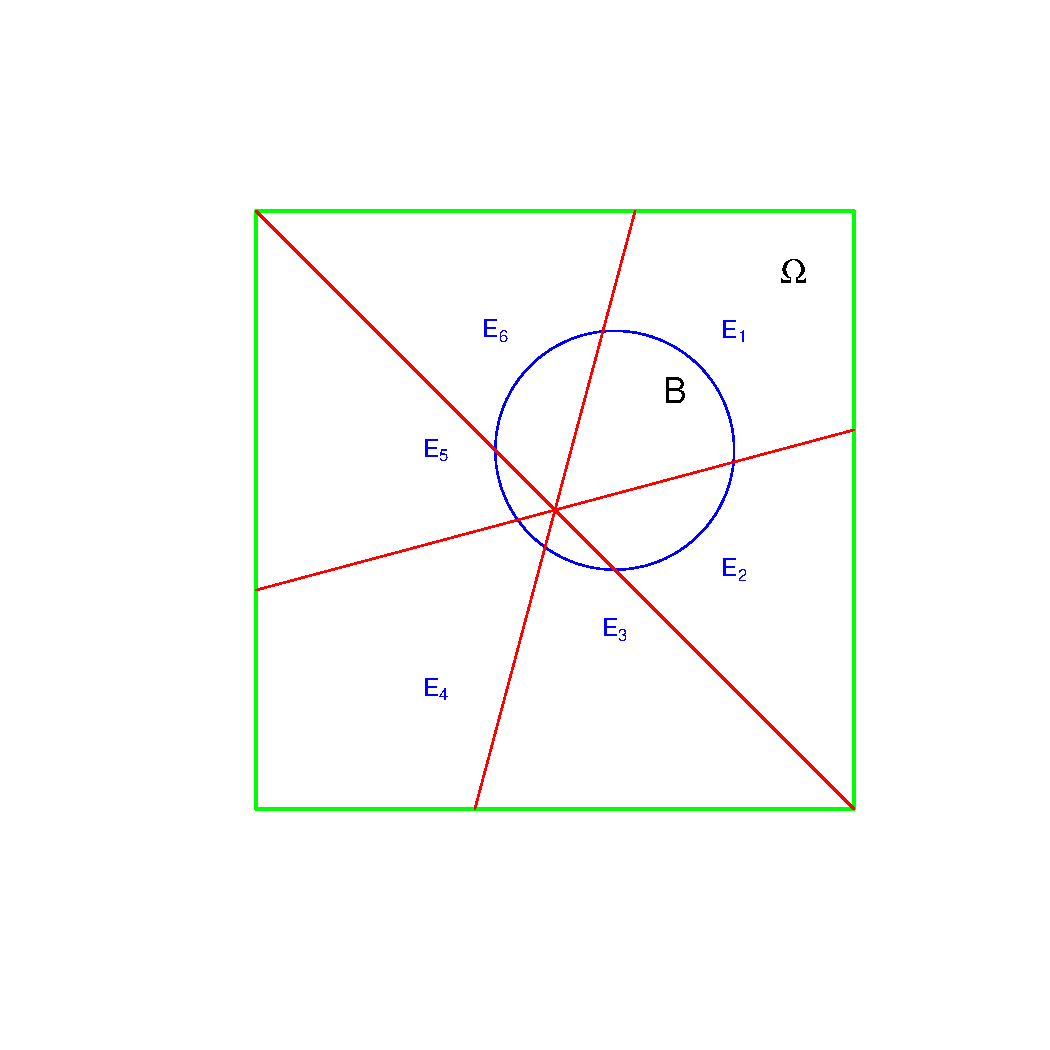
\includegraphics[width=\maxwidth]{figure/r-1} 

\end{knitrout}
$$B=(B\cap E_1)\cup (B\cap E_2)\cup\ldots \cup (B\cap E_N)$$
E quindi

$$P(B)=P(B\cap E_1)+P(B\cap E_2)+\ldots+ P(B\cap E_N)=$$
$$ P(B\mid E_1)P(E_1)+\ldots+P(B\mid E_N)P(E_N)$$

\subsection{Esempio}

$$B=\textrm{piove}$$
$$E_1 = \textrm{vado a lezione}$$
$$E_2 = \textrm{non vado a lezione}$$
$$P(\textrm{piove}) = P(\textrm{piove e vado a lezione}) + P(\textrm{piove e non vado a lezione}) $$ 

 

\section{Teorema di Bayes [forma estesa]}

Combinando con la regola di Bayes:

$$P (E_i\mid B) = \dfrac{P(B\mid E_i) P(E_i)}{P(B)}= \dfrac{P(B\mid E_i ) P(E_i) }{ 
\sum_{i=1}^N P(B\mid E_i)P(E_i)}$$

Nel caso particolare in cui gli eventi possibili 
$E_1$ e $E_2$ siano $A$ e il suo complemento  $A^C$ si ha

$$P (A|B)=  \dfrac{P[B\mid A] P(A)}{P (B\mid A) P(A)+P(B\mid  A^C) P( A^C)}$$


 
 


\section{La concezione frequentista}
 

\subsection{Lancio di una coppia di dadi}

\begin{knitrout}
\definecolor{shadecolor}{rgb}{0.969, 0.969, 0.969}\color{fgcolor}\begin{kframe}
\begin{verbatim}
## x
##    2    3    4    5    6    7    8    9   10   11   12 
##  298  582  770 1127 1371 1683 1356 1131  819  575  288
\end{verbatim}
\end{kframe}
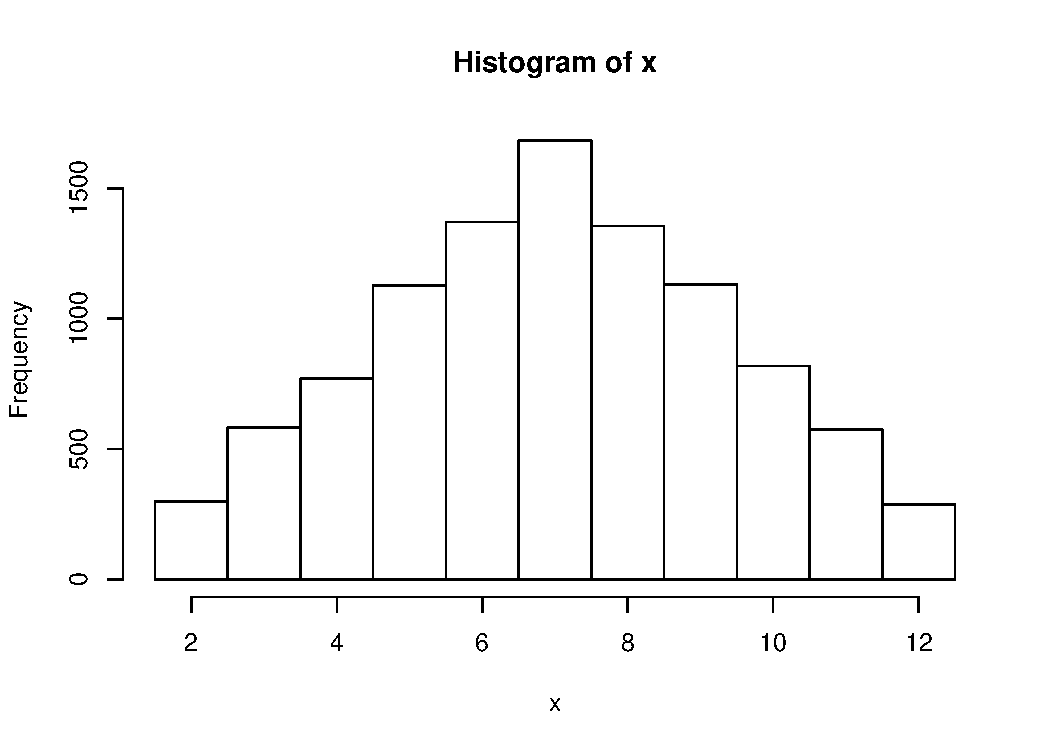
\includegraphics[width=\maxwidth]{figure/unnamed-chunk-14-1} 

\end{knitrout}

 

\begin{knitrout}
\definecolor{shadecolor}{rgb}{0.969, 0.969, 0.969}\color{fgcolor}\begin{kframe}
\begin{alltt}
\hlstd{y}
\end{alltt}
\begin{verbatim}
## x
##    2    3    4    5    6    7    8    9   10   11   12 
##  298  582  770 1127 1371 1683 1356 1131  819  575  288
\end{verbatim}
\end{kframe}
\end{knitrout}
Il numero 8 è uscito in questo caso k=1356 volte su N= 10000 lanci.  
Possiamo dire che il risultato esce di norma k  volte su 10000 e scrivere 

$$\textit{Probabilità che esca 8}=\lim_{N\to \infty}\dfrac{k}{N}$$
 
Il valore stimato con 10000 lanci è

$$\textrm{probabilità che esca 8} \approx 1356/10000 = 0.1356$$

 


Vedremo in seguito che

$$\textrm{Probabilità che esca 8} = 5/36=0.1389 $$

e quindi che la differenza relativa della nostra stima dal valor vero è di 

$$\dfrac{0.1356 -0.1389}{0.1389}=\ensuremath{-0.0237581}$$

ovvero la discrepanza relativa è circa del 2.4%.  

Stimiamo la probabilità di un evento A come la frequenza relativa dell'evento
$$P(A)\approx \dfrac{\textrm{numero di volte in cui l'evento si realizza}}{\textrm{numero di esperimenti 
eseguiti}}$$

 

Questa concezione ``frequentista`` della probabilità è sufficiente in tutti i casi in cui l'esperimento può essere ripetuto  (almeno a livello concettuale) quante volte si vuole.
Non è però sufficiente per i casi in cui l'esperimento non può essere ripetuto o forse nemmeno eseguito. 

 In tali casi si ricorre alla concezione \emph{soggettiva} della probabilità, in cui la probabilità viene stimata da un soggetto sulla base dell'esperienza personale. 


\subsection{Esercizio 1 }



Due urne contengono palle colorate. La prima urna contiene  50
palle rosse e 50 palle blu. La seconda contiene 30 palle rosse e 70 blu. Si sceglie una delle due urne a caso e si estrae da questa una palla a caso.  
La palla   estratta  è rossa. 
Quale è la probabilità che la palla provenga della prima urna?



\subsection{Albero di probabilità}

\begin{knitrout}
\definecolor{shadecolor}{rgb}{0.969, 0.969, 0.969}\color{fgcolor}
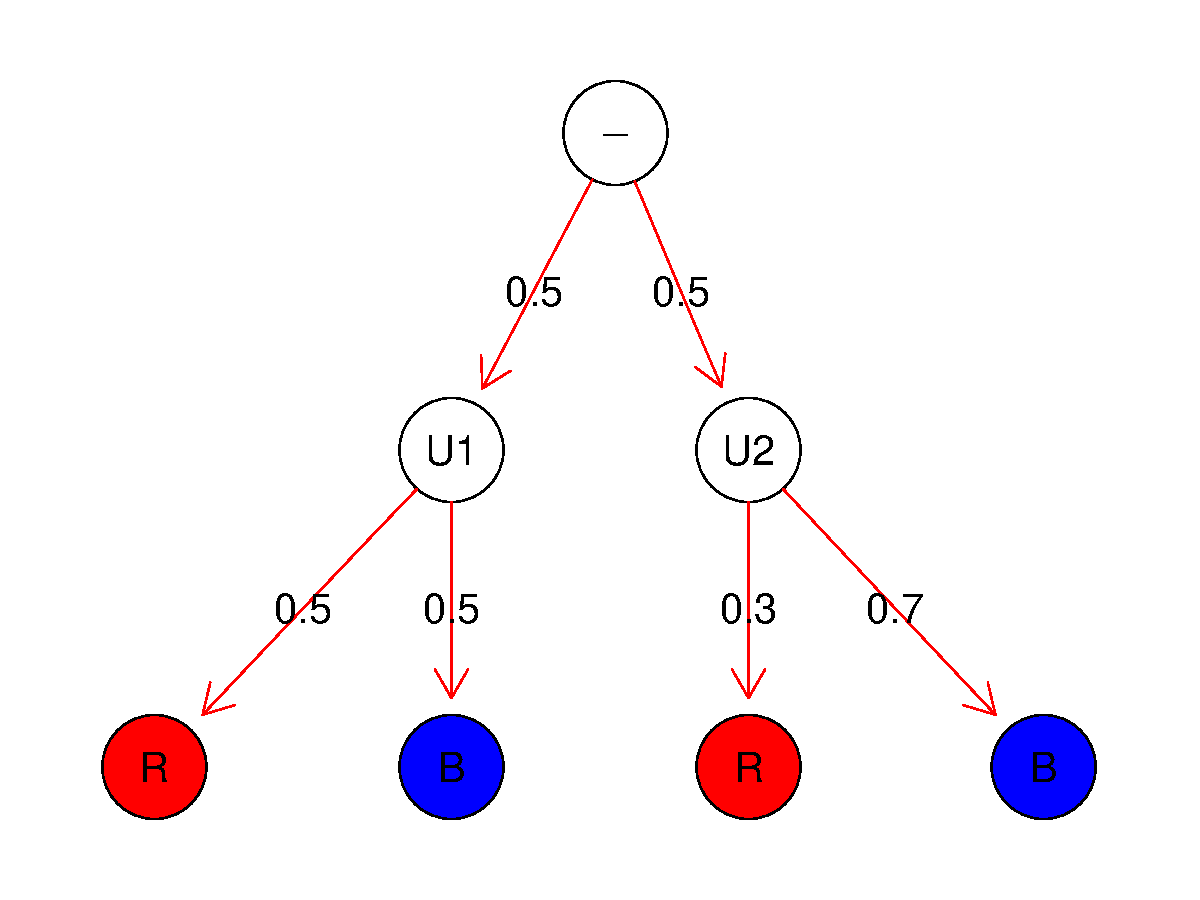
\includegraphics[width=\maxwidth]{figure/unnamed-chunk-18-1} 

\end{knitrout}

Motliplicando i valori delle frecce che puntano ad una foglia si trova
$$P(R\mid U1)P(U_1)=0.5\times 0.5=P(R\cap U1)$$
$$P(R\mid U2)P(U_2)=0.5\times 0.3=P(R\cap U2)$$
e quindi per esempio
$$P(R)=P(R\cap U1)+P(R\cap U2)=0.4$$
Usando poi la regola di Bayes
$$P(U_1\mid R)=\dfrac{P(R\mid U_1)P(U_1)}{P(R)}=0.25/0.4=5/8$$


\subsection{Esempio 2}

Consideriamo dei container per la raccolta di materiale tossico. I container potrebbero non avere una tenuta perfetta ed avere delle perdite. Un programma di monitoraggio  controlla regolarmente se ci sono state perdite. Gli strumenti dedicati a tali controlli non sono perfetti e talora danno luogo a falsi positivi o falsi negativi.  In altre parole a volte viene emesso un segnale d'allarme quando non si ha perdita (falso positivo) a volte la perdita non viene segnalata quando c'è (falso negativo).

Assumiamo di avere 3 informazioni

Informazioni sui container

1.   P (perdita)= 0.1    
     P (nessuna perdita)=0.9

Per quanto riguarda il test

2.   P(test positivo | perdita)=P (analisi corretta se si ha perdita)=0.95

     P(test negativo | perdita)=P(test negativo dato che  si ha perdita) =  0.05  (falsi negativi)

3.   P(test positivo | non perdita)=P(test positivo quando non si ha perdita) =    0.1  (falso positivo)
      
      P(test negativo| non perdita)=P(non rilevamento quando non si ha perdita)=0.9
      

Vorremmo rispondere alle seguenti 2 domande.

1.  Se l'allarme scatta quale è la probabilità che ci sia stata effettivamente una perdita?

2.  Se l'allarme non scatta quale è la probabilità che il sito sia invece contaminato?

Costruiamo un diagramma ad albero come prima

---



\begin{knitrout}
\definecolor{shadecolor}{rgb}{0.969, 0.969, 0.969}\color{fgcolor}
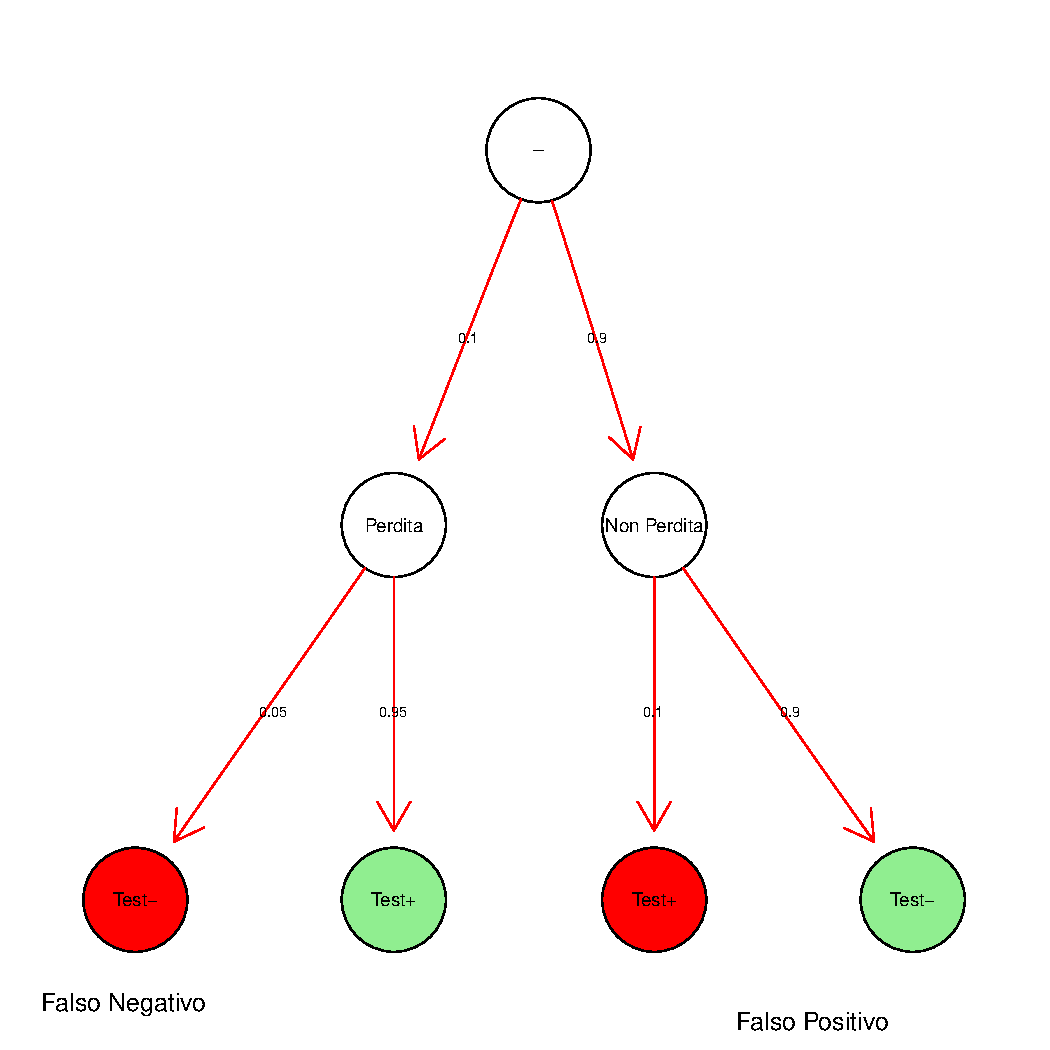
\includegraphics[width=\maxwidth]{figure/unnamed-chunk-20-1} 

\end{knitrout}

$$P(\textrm{positivo})=0.1\times 0.95+0.1\times 0.9=0.185$$
e utilizzando la regola di Bayes

$$P(\textrm{perdita}\mid \textrm{positivo})=\dfrac{P(\textrm{positivo}\mid \textrm{perdita})P(\textrm{perdita})}{P(\textrm{positivo})}=0.095/0.185=0.5135135$$


$$P(\textrm{perdita}\mid \textrm{negativo})=\dfrac{P(\textrm{negativo}\mid \textrm{perdita})P(\textrm{perdita})}{P(\textrm{negativo})}=0.005/0.815=0.006135$$
\subsection{Esempio 3: specificità e sensitività di un test diagnostico }

\subsubsection{Sensitività }

"proporzione dei positivi identificati tra i malati: 
indica la capacità di individuare malati"


$$P(+ \mid D)=P(\textrm{test positivo}\mid \textrm{malato})$$
Supponiamo sia


$$P(\textrm{test positivo | malato}) = 0.97$$
$$P(\textrm{test negativo} \mid  \textrm{malato}) = 0.03 \textrm{ (Falsi Negativi)}$$

\subsubsection{Specificità }

"proporzione dei negativi identificati: indica la capacità di individuare i sani" 
$$P(-\mid D^c)= P(\textrm{test negativo | sano})$$

Supponiamo sia
$$P(\textrm{test negativo | sano}) = 0.95$$
$$P(\textrm{test positivo | sano}) = 0.05 \quad \hbox{(Falsi positivi)}$$

* Supponiamo di essere testati per una malattia che colpisce lo 0.1\%  della popolazione. 
* Determinare  probabilità  di non avere la malattia avendo avuto un esito positivo del test.
In formule 
$$P (\textrm{sani | test positivo}) = ?$$
$$P(\textrm{malati | test negativo})=?$$
 
\subsection{Albero sensitività/specificità}




\begin{knitrout}
\definecolor{shadecolor}{rgb}{0.969, 0.969, 0.969}\color{fgcolor}
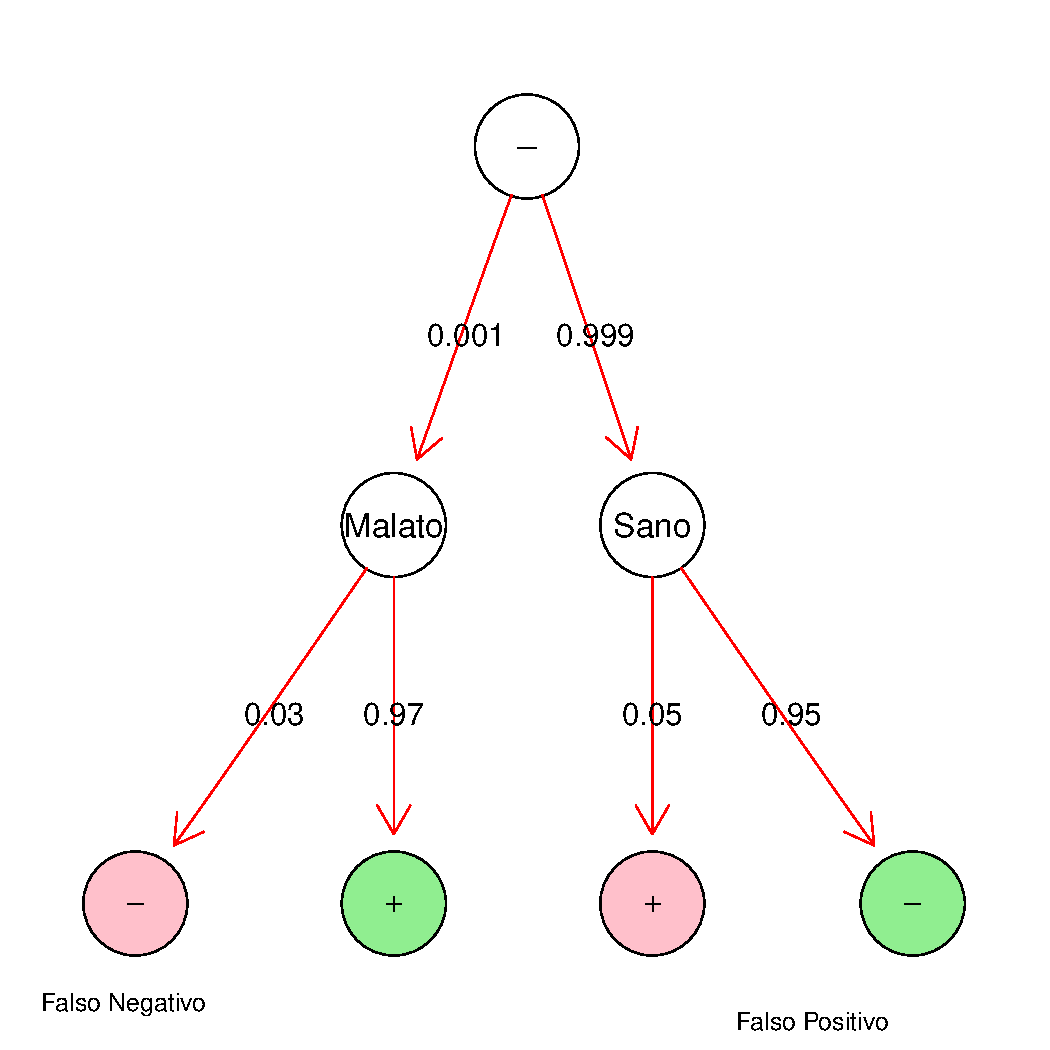
\includegraphics[width=\maxwidth]{figure/unnamed-chunk-23-1} 

\end{knitrout}

\begin{align*}P(+) &= P(+ \mid  \textrm{sano})P(\textrm{sano}) + P( + \mid \textrm{malato})P(\textrm{malato}) \\
&=0.05\times 0.999 + 0.97\times  0.001=0.05092
\end{align*}
 

$$ P(\textrm{sano} \mid   +) = \dfrac{P( +\mid  \textrm{sano}) P(\textrm{sano})}{P(+)}=\dfrac{0.05*0.999}{0.05092}=0.9809505$$


 


In genere
$$P(+) = \hbox{(1-specificità)(1-prevalenza) + sensitività prevalenza}$$



\begin{knitrout}
\definecolor{shadecolor}{rgb}{0.969, 0.969, 0.969}\color{fgcolor}
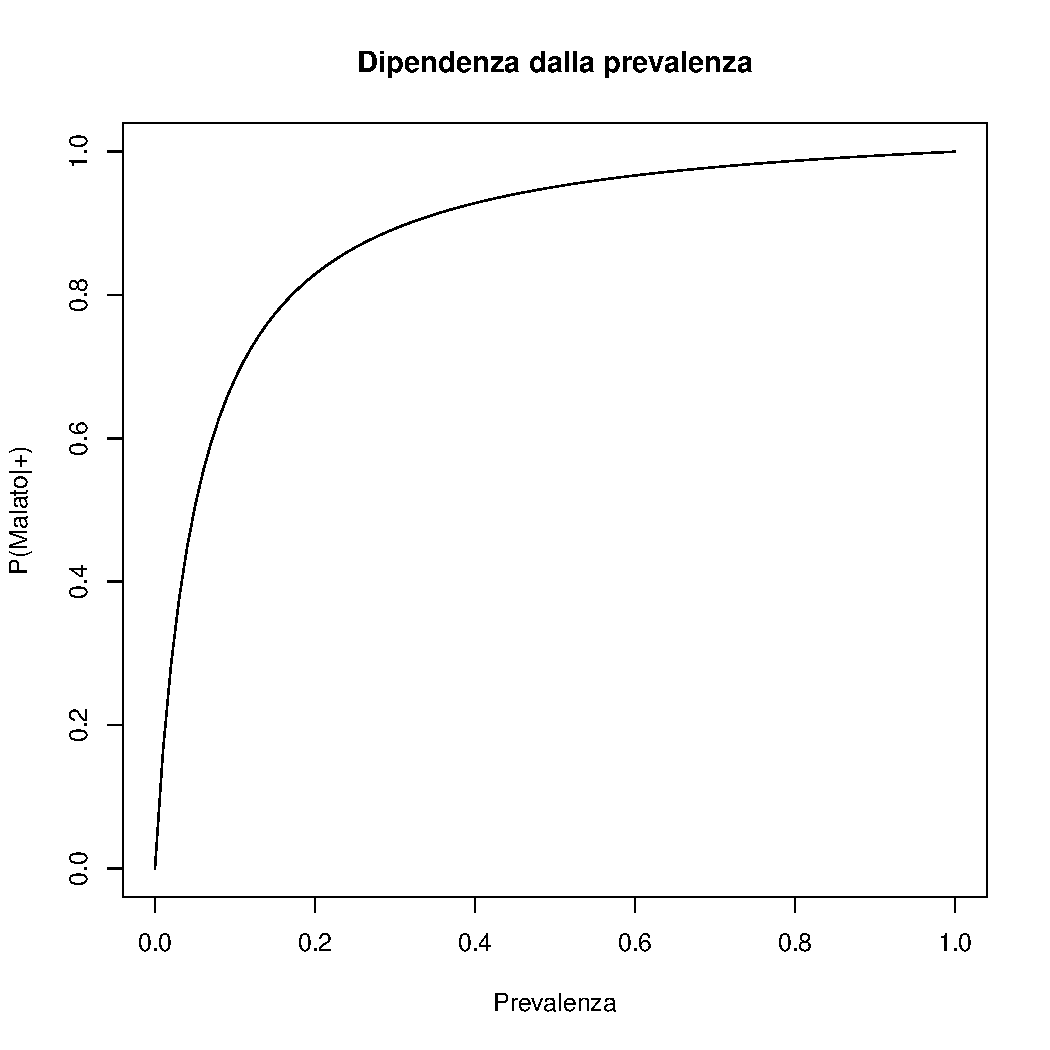
\includegraphics[width=\maxwidth]{figure/unnamed-chunk-24-1} 

\end{knitrout}



\subsection{Approccio frequentista}
Immaginando $10^6$ soggetti

\begin{knitrout}
\definecolor{shadecolor}{rgb}{0.969, 0.969, 0.969}\color{fgcolor}\begin{kframe}
\begin{verbatim}
##         Test - Test +  Totali
## Affetti             -        
## Sani         -      -       -
## Totali              - 1000000
## Usando la prevalenza
##         Test - Test +  Totali
## Affetti      -      -    1000
## Sani         -      -  999000
## Totali       -      - 1000000
## Usando la sensitivita'
##         Test - Test +  Totali
## Affetti     30    970    1000
## Sani                   999000
## Totali                1000000
## Usando la specificita'
##         Test - Test +  Totali
## Affetti     30    970    1000
## Sani    949050  49950  999000
## Totali                1000000
## Calcolando i totali
##         Test - Test +  Totali
## Affetti     30    970    1000
## Sani    949050  49950  999000
## Totali  949080  50920 1000000
\end{verbatim}
\end{kframe}
\end{knitrout}


$$P (\textrm{affetti | test negativo}) = 30/949080=0.0000316$$
        
        
        
        
\subsubsection{Terminologia}
        
Il \emph{valore predittivo positivo} è  (D sta per disease)

$$P (D \mid +)$$
        
Il \emph{valore predittivo negativo} è 

$$P (D^c \mid  -)$$
        
probabilità di non avere la malattia assunto un esito   negativo del test. 

La \emph{prevalenza} di una malattia è

$$P(D)$$
        
Il \emph{rapporto di verosimiglianza diagnostico di un test positivo} $DLR_+$ è

$$\frac{P (+\mid D)}{P(+\mid D^c)}=\frac{\textrm{sensitivita}}{1-\textrm{specificità}}$$
        
Il \emph{rapporto di  verosimiglianza diagnostico di un test negativo}   $DLR_-$  è

$$ \frac{P (-\mid D)}{P(-\mid D^c)}=\frac{1-\textrm{sensitivita}}{\textrm{specificita}}$$
        
\subsection{HIV}
        
Uno studio sull'efficacia dei test HIV riporta un test con sensitività 
$P(+|\textrm{malato})=99.7\%$ e specificità $P(-|\textrm{sano})= 98.5\%$ .
Supponiamo  che la prevalenza dell'HIV sia dello 0.1\%. 
Determinare la probabilità  $P(D|+)$, che un soggetto (positivo al test) abbia l'HIV.

Calcolare inoltre 
$P(D^c|-)$ e $P(D)$

$$P (+) =  P (+| D) P (D) + P (+| S) P (S)  =0.997\times 0.001 + 0.015\times 0.999 = 0.015982$$

$$P (D | +) = P (+| D) P (D)/P (+) = 0.997\times 0.001/0.015982 =0.0623827$$

\subsubsection{ Test di gravidanza}


Un sito web \url{http://www.medicine.ox.ac.uk/bandolier/band64/b64-7.html} per test di gravidanza afferma:  


"Quando i soggetti che hanno effettuato i test erano le donne che hanno raccolto e analizzato i loro campioni la sensitività  era del 75\%. La specificità era anche bassa, nel range dal 52\% al 75\%." 

Consideriamo il valore inferiore della specificità.  Supponiamo che il risultato sia negativo e che il 30\%  delle donne che fanno il test  siano effettivamente pregnanti. Determinare la probabilità di essere incinte dato il risultato negativo del test?

$$P (\textrm{Incinta }\mid -) = \dfrac{P (-\mid \textrm{Incinta}) P (\textrm{Incinta})}{P (-)} =$$
$$\dfrac{ P (-\mid \textrm{Incinta}) P (\textrm{incinta})}{(P (-\mid \textrm{Incinta}) P (\textrm{Incinta}) + P (-\mid \textrm{Non Incinta}) P (\textrm{Non Incinta})}=$$

$$0.250*0.3 /(0.250*0.3 + 0.52*0.7)=0.1708428$$



\subsubsection{Fallacia del Pubblico Ministero}


Supponiamo  che in una comunità di 10 abitanti sia stato commesso un delitto. Il colpevole è un abitante della comunità (immediatamente isolata).


Immaginiamo che da un test del sangue si trovi che un abitante individuato in modo casuale  (il sospettato) e il colpevole condividano una caratteristica comune allo 5% della popolazione (match con probabilità  0.05). 

Il pubblico ministero afferma che la probabilità di essere innocente del sospettato è dello 5% (0.05).


In realtà (indicando con G la colpevolezza e I l'innocenza)

$$P (\textrm{G}\mid\textrm{test}) 
= P (\textrm{test}\mid\textrm{ G})P (\textrm{G})/P (\textrm{test})$$
        
$$P (\textrm{test} \mid \textrm{G}) = 1\quad 
P (\textrm{G}) = 1/10$$
        
$$P (\textrm{test}) = P(\textrm{test}\mid  \textrm{G}) P(\textrm{G}) +
P(\textrm{test}\mid\textrm{I})P(\textrm{I}) =
1*1/10 + 0.05 *9/10 = 0.145$$
        
Quindi

$$P (\textrm{G}\mid\textrm{test}) = 0.1/0.145=
        0.6896552$$
        
       
        
        
\subsubsection{Odds}
        
Si definiscono le <b>odds</b> di un evento

$$\textrm{Odds}(E) = \frac{P(E)}{P(\textrm{not E})}= \frac{P(E)}{1 - P(E)}$$
        
Il logaritmo naturale delle odds è detto 
<b>logit</b>. Il rapporto tra due odds è detto <b>odds ratio</b>.

\subsubsection{Il  problema delle 3 porte (Monty Hall problem)}

Ci sono 3 porte. Dietro a 2 delle 3 porte una capra. Dietro alla restante una Ferrari.  Il giocatore sceglie una porta (ma non la fa aprire). Il conduttore ne apre una delle altre 2 mostrando una capra  e chiede al giocatore se vuole cambiare la sua scelta originale.
Conviene attenersi alla scelta originale o conviene cambiare? 

Supponiamo per concretezza che che si sia deciso di aprire la porta 1  e che il presentatore apra la 3. Poniamo B="il presentatore apre la 3". Conviene scegliere al porta 2 (e cambiare la nostra scelta iniziale) o restare ostinati e scegliere la porta 1?


$F_1$ è  l'evento "la Ferrari è dietro alla porta 1",  $F_2$ e $F_3$ sono definiti in modo uguale con le porte 2 e 3 rispettivamente.  Per esempio, abbiamo scelto la porta 1  


\begin{knitrout}
\definecolor{shadecolor}{rgb}{0.969, 0.969, 0.969}\color{fgcolor}\begin{kframe}
\begin{alltt}
\hlkwd{library}\hlstd{(MASS)}
\hlstd{a1}\hlkwb{=}\hlkwd{fractions}\hlstd{(}\hlnum{1}\hlopt{/}\hlnum{3}\hlstd{)}
\hlstd{a2}\hlkwb{=}\hlkwd{fractions}\hlstd{(}\hlnum{1}\hlopt{/}\hlnum{3}\hlstd{)}
\hlstd{a3}\hlkwb{=}\hlkwd{fractions}\hlstd{(}\hlnum{1}\hlopt{/}\hlnum{3}\hlstd{)}
\hlstd{a11}\hlkwb{=}\hlnum{1}\hlopt{/}\hlnum{2}
\hlstd{a12}\hlkwb{=}\hlnum{1}\hlopt{/}\hlnum{2}
\hlstd{a21}\hlkwb{=}\hlnum{1}
\hlstd{a22}\hlkwb{=}\hlnum{0}
\hlstd{a31}\hlkwb{=}\hlnum{0}
\hlstd{a32}\hlkwb{=}\hlnum{1}
\hlstd{p11}\hlkwb{=}\hlstd{a1}\hlopt{*}\hlstd{a11}
\hlstd{p12}\hlkwb{=}\hlstd{a1}\hlopt{*}\hlstd{a12}
\hlstd{p21}\hlkwb{=}\hlstd{a2}\hlopt{*}\hlstd{a21}
\hlstd{p22}\hlkwb{=}\hlstd{a2}\hlopt{*}\hlstd{a22}
\hlstd{p31}\hlkwb{=}\hlstd{a3}\hlopt{*}\hlstd{a31}
\hlstd{p32}\hlkwb{=}\hlstd{a3}\hlopt{*}\hlstd{a32}
\hlstd{node1}\hlkwb{<-}\hlstr{"_"}
\hlstd{node2}\hlkwb{<-}\hlstr{"F1"}
\hlstd{node3}\hlkwb{<-}\hlstr{"F2"}
\hlstd{node4}\hlkwb{<-}\hlstr{"F3"}
\hlstd{node5}\hlkwb{<-}\hlstr{"RU1"}
\hlstd{node6}\hlkwb{<-}\hlstr{"BU1"}
\hlstd{node7}\hlkwb{<-}\hlstr{"RU2"}
\hlstd{node8}\hlkwb{<-}\hlstr{"BU2"}
\hlstd{node9}\hlkwb{<-}\hlstr{"RU3"}
\hlstd{node10}\hlkwb{<-}\hlstr{"BU3"}
\hlstd{nodeNames}\hlkwb{<-}\hlkwd{c}\hlstd{(node1,node2,node3,node4, node5,node6, node7,node8,node9,node10)}

\hlstd{rEG} \hlkwb{<-} \hlkwd{new}\hlstd{(}\hlstr{"graphNEL"}\hlstd{,} \hlkwc{nodes}\hlstd{=nodeNames,} \hlkwc{edgemode}\hlstd{=}\hlstr{"directed"}\hlstd{)}
\hlcom{# Draw the "lines" or "branches" of the probability Tree}
\hlstd{rEG} \hlkwb{<-} \hlkwd{addEdge}\hlstd{(nodeNames[}\hlnum{1}\hlstd{], nodeNames[}\hlnum{2}\hlstd{], rEG,} \hlnum{1}\hlstd{)}
\hlstd{rEG} \hlkwb{<-} \hlkwd{addEdge}\hlstd{(nodeNames[}\hlnum{1}\hlstd{], nodeNames[}\hlnum{3}\hlstd{], rEG,} \hlnum{1}\hlstd{)}
\hlstd{rEG} \hlkwb{<-} \hlkwd{addEdge}\hlstd{(nodeNames[}\hlnum{1}\hlstd{], nodeNames[}\hlnum{4}\hlstd{], rEG,} \hlnum{1}\hlstd{)}
\hlstd{rEG} \hlkwb{<-} \hlkwd{addEdge}\hlstd{(nodeNames[}\hlnum{2}\hlstd{], nodeNames[}\hlnum{5}\hlstd{], rEG,} \hlnum{1}\hlstd{)}
\hlstd{rEG} \hlkwb{<-} \hlkwd{addEdge}\hlstd{(nodeNames[}\hlnum{2}\hlstd{], nodeNames[}\hlnum{6}\hlstd{], rEG,} \hlnum{1}\hlstd{)}
\hlstd{rEG} \hlkwb{<-} \hlkwd{addEdge}\hlstd{(nodeNames[}\hlnum{3}\hlstd{], nodeNames[}\hlnum{7}\hlstd{], rEG,} \hlnum{10}\hlstd{)}
\hlstd{rEG} \hlkwb{<-} \hlkwd{addEdge}\hlstd{(nodeNames[}\hlnum{3}\hlstd{], nodeNames[}\hlnum{8}\hlstd{], rEG,} \hlnum{10}\hlstd{)}
\hlstd{rEG} \hlkwb{<-} \hlkwd{addEdge}\hlstd{(nodeNames[}\hlnum{4}\hlstd{], nodeNames[}\hlnum{9}\hlstd{], rEG,} \hlnum{10}\hlstd{)}
\hlstd{rEG} \hlkwb{<-} \hlkwd{addEdge}\hlstd{(nodeNames[}\hlnum{4}\hlstd{], nodeNames[}\hlnum{10}\hlstd{], rEG,} \hlnum{10}\hlstd{)}
\hlstd{eAttrs} \hlkwb{<-} \hlkwd{list}\hlstd{()}
\hlstd{nAttrs}\hlkwb{<-}\hlkwd{list}\hlstd{()}
\hlstd{q}\hlkwb{<-}\hlkwd{edgeNames}\hlstd{(rEG)}
\hlstd{nAttrs}\hlopt{$}\hlstd{fillcolor}\hlkwb{=}\hlkwd{rep}\hlstd{(}\hlstr{"light green"}\hlstd{,}\hlnum{10}\hlstd{)}
\hlkwd{names}\hlstd{(nAttrs}\hlopt{$}\hlstd{fillcolor)} \hlkwb{<-} \hlstd{nodeNames}
\hlstd{nAttrs}\hlopt{$}\hlstd{label}\hlkwb{=}\hlkwd{c}\hlstd{(}\hlstr{"_"}\hlstd{,}\hlstr{"F1"}\hlstd{,}\hlstr{"F2"}\hlstd{,}\hlstr{"F3"}\hlstd{,}\hlstr{"B"}\hlstd{,}\hlstr{"non B"}\hlstd{,}\hlstr{"B"}\hlstd{,}\hlstr{"non B"}\hlstd{,}\hlstr{"B"}\hlstd{,}\hlstr{"non B"}\hlstd{)}
\hlkwd{names}\hlstd{(nAttrs}\hlopt{$}\hlstd{label)} \hlkwb{<-} \hlstd{nodeNames}
\hlcom{# Add the probability values to the the branch lines}

\hlstd{eAttrs}\hlopt{$}\hlstd{label} \hlkwb{<-} \hlkwd{c}\hlstd{(}\hlkwd{toString}\hlstd{(a1),}\hlkwd{toString}\hlstd{(a2),}
\hlkwd{toString}\hlstd{(a3),} \hlkwd{toString}\hlstd{(a11),}
\hlkwd{toString}\hlstd{(a12),} \hlkwd{toString}\hlstd{(a21),} \hlkwd{toString}\hlstd{(a22),} \hlkwd{toString}\hlstd{(a31),} \hlkwd{toString}\hlstd{(a32))}
\hlkwd{names}\hlstd{(eAttrs}\hlopt{$}\hlstd{label)} \hlkwb{<-} \hlkwd{c}\hlstd{(q[}\hlnum{1}\hlstd{],q[}\hlnum{2}\hlstd{], q[}\hlnum{3}\hlstd{], q[}\hlnum{4}\hlstd{], q[}\hlnum{5}\hlstd{], q[}\hlnum{6}\hlstd{],q[}\hlnum{7}\hlstd{],q[}\hlnum{8}\hlstd{],q[}\hlnum{9}\hlstd{])}
\hlstd{edgeAttrs}\hlkwb{<-}\hlstd{eAttrs}
\hlstd{nodeAttrs}\hlkwb{<-}\hlstd{nAttrs}
\hlcom{# Set the color, etc, of the tree}
\hlstd{attributes}\hlkwb{<-}\hlkwd{list}\hlstd{(}\hlkwc{node}\hlstd{=}\hlkwd{list}\hlstd{(}\hlkwc{label}\hlstd{=}\hlstr{"foo"}\hlstd{,} \hlkwc{fontsize}\hlstd{=}\hlstr{"15"}\hlstd{),}
\hlkwc{edge}\hlstd{=}\hlkwd{list}\hlstd{(}\hlkwc{color}\hlstd{=}\hlstr{"red"}\hlstd{),}\hlkwc{graph}\hlstd{=}\hlkwd{list}\hlstd{(}\hlkwc{rankdir}\hlstd{=}\hlstr{"TD"}\hlstd{))}
\end{alltt}
\end{kframe}
\end{knitrout}




$$P(F_1)=P(F_2)=P(F_3) = 1/3$$
$$P(B) = 1/2$$
$$P(B \mid F_1) = 1/2$$
$$P(B \mid  F_2) = 1$$
$$P(B \mid  F_3) = 0$$

Possiamo quindi calcolare

$$P(F_1  \mid B) = \frac{P(B \mid F_1)P(F_1)}{P(B) }= \frac{1/2*1/3}{1/2} = 1/3$$
$$P(F_2  \mid B) = \frac{P(B  \mid F_2)P(F_2)}{P(B)} =\frac{1*1/3}{1/2} = 2/3$$
$$P(F_3  \mid B) = \frac{P(B \mid F_3)P(F_3)}{P(B)} = 0$$

\subsubsection{Grafico}


<<echo=FALSE>=
plot(rEG, edgeAttrs=eAttrs, nodeAttrs=nAttrs,attrs=attributes)
@


\section{Recessione}

Una agenzia economica ha creato un modello che predice recessione. Il modello predice recessione con probabilità del 80\% quando  la recessione sta effettivamente arrivando e con probabilità del 10\% quando la recessione non sta arrivando. La probabilità che la recessione sia in arrivo è del 20\%. Se il modello predice recessione quale è la probabilità che la recessione stia effettivamente arrivando?

P(Prevista) = P(Prevista | Recessione)P(Recessione) + P(Prevista | No recessione) P(No Recessione) =$0.8\times 0.2 + 0.1\times 0.8$=0.24



P(Recessione | Prevista) = P(Prevista | Recessione)*P(Recessione)/P(Prevista)=$0.8\times 0.2/0.24$=0.6666667



\subsection{Esercizio} 

Alice ha 2 monete nella borsa. La prima con 2 facce diverse e la seconda con 2 teste. Alice preleva a caso una moneta dalla borsa. La lancia e vede testa. Quale è la probabilità che abbia lanciato la moneta equa?


 
 
\section{Simulazioni}


Come possiamo simulare variabili aventi valore nell'alfabeto assegnato?
In effetti qualunque comando di generazione su un computer non \`e perfettamente casuale; infatti la generazione avviene in effetti in modo pseudo-casuale e  secondo un meccanismo che dipende dallo stato interno del computer codificato in una variabile indicata con \texttt{.Random.seed}. Se il {\it seme} iniziale \`e lo stesso i numeri generati saranno uguali. Spesso conviene che i calcoli (ad esempio a fine didattico) siano riproducibili. Ad esempio mettendo in una variabile \texttt{seme} il valore corrente di \texttt{.Random.seed} e richiamandolo o generandolo all'occorrenza.  
Un altro modo di procedere consiste nell'impostare il valore di 
\texttt{.Random.seed} attraverso il comando 
\texttt{set.seed}  la cui sintassi \`e 
$\texttt{set.seed}(\varia{n})$ dove $n$ \`e un numero intero.
 
\begin{knitrout}
\definecolor{shadecolor}{rgb}{0.969, 0.969, 0.969}\color{fgcolor}\begin{kframe}
\begin{alltt}
\hlkwd{set.seed}\hlstd{(}\hlnum{3}\hlstd{)}
\end{alltt}
\end{kframe}
\end{knitrout}
 
A questo punto possiamo simulare le variabili richieste usando la struttura
\begin{equation}\texttt{sample}(\varia{alfabeto},\varia{n})\end{equation}
Se l'alfabeto consiste di tutte le lettere minuscole dell'alfabeto ordinario e ne vogliamo selezionare $n=8$  (in modo che ciascun uscita abbia la stessa probabilit\`a)  basta scrivere
\begin{knitrout}
\definecolor{shadecolor}{rgb}{0.969, 0.969, 0.969}\color{fgcolor}\begin{kframe}
\begin{alltt}
\hlkwd{sample}\hlstd{(letters,}\hlnum{8}\hlstd{)}
\end{alltt}
\begin{verbatim}
## [1] "e" "u" "j" "h" "n" "m" "c" "f"
\end{verbatim}
\end{kframe}
\end{knitrout}
Se invece l'alfabeto consiste delle basi del DNA
\begin{knitrout}
\definecolor{shadecolor}{rgb}{0.969, 0.969, 0.969}\color{fgcolor}\begin{kframe}
\begin{alltt}
\hlstd{alfabeto}\hlkwb{=}\hlkwd{c}\hlstd{(}\hlstr{"A"}\hlstd{,}\hlstr{"C"}\hlstd{,}\hlstr{"G"}\hlstd{,}\hlstr{"T"}\hlstd{)}
\hlkwd{sample}\hlstd{(alfabeto,}\hlnum{2}\hlstd{)}
\end{alltt}
\begin{verbatim}
## [1] "G" "C"
\end{verbatim}
\end{kframe}
\end{knitrout}
Notiamo che
\begin{knitrout}
\definecolor{shadecolor}{rgb}{0.969, 0.969, 0.969}\color{fgcolor}\begin{kframe}
\begin{alltt}
 \hlkwd{sample}\hlstd{(alfabeto)}
\end{alltt}
\begin{verbatim}
## [1] "G" "C" "T" "A"
\end{verbatim}
\end{kframe}
\end{knitrout}
restituisce una permutazione dell'alfabeto, mentre chiedendo un campione di lunghezza superiore alla lunghezza dell'alfabeto otteniamo un messaggio di errore. Possiamo per\`o immaginare di re-immettere la lettera estratta nell'urna dopo ogni estrazione. In questo caso non c'\`e limite alla sequenza generata.
Per esempio
\begin{knitrout}
\definecolor{shadecolor}{rgb}{0.969, 0.969, 0.969}\color{fgcolor}\begin{kframe}
\begin{alltt}
\hlstd{alfabeto}\hlkwb{=}\hlkwd{c}\hlstd{(}\hlstr{"testa"}\hlstd{,}\hlstr{"croce"}\hlstd{)}
\hlkwd{sample}\hlstd{(alfabeto,}\hlnum{5}\hlstd{,}\hlkwc{replace}\hlstd{=T)}
\end{alltt}
\begin{verbatim}
## [1] "croce" "croce" "testa" "croce" "croce"
\end{verbatim}
\end{kframe}
\end{knitrout}
 

Il precursore  del dado era chiamato \emph{astragalo} ed era giocato nell'antica Grecia e nell'antica Roma~\cite{david}.
Gli  astragali sono dei piccoli ossicini di forma irregolare ed hanno 6 facce ma atterranno in  modo stabile solo su 4 di esse numerate 1, 3, 4 e 6  con probabilit\`a all'incirca 0.4 per il 3 e il 4  e di 0.1 per l'1 e il 6. In altre parole l'astragalo \`e descritto dalla tabella

\begin{center}\begin{tabular}{|r|r |}
\hline
 valore&  probabilit\`a \\
\hline
1&0.1\\
3 &0.4\\
4& 0.4\\
6&0.1\\
 \hline
\end{tabular}
\end{center}
Il tiro pi\`u gettonato all'epoca era l'uscita di 4 facce diverse nel lancio di 4 astragali e si chiamava {\it Venus}.
Il lancio considerato peggiore sul singolo lancio era l'1 chiamato cane o avvoltoio.
\begin{figure}[htbp]
\begin{center}
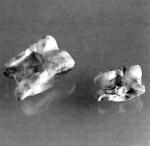
\includegraphics[width=6cm]{../grafici/astragals.jpeg}
\caption{ Astragalo. }
\label{fig:astragalo}
\end{center}
\end{figure}
Per simulare un astragalo su un computer
\begin{knitrout}
\definecolor{shadecolor}{rgb}{0.969, 0.969, 0.969}\color{fgcolor}\begin{kframe}
\begin{alltt}
\hlkwd{sample}\hlstd{(}\hlkwd{c}\hlstd{(}\hlnum{1}\hlstd{,}\hlnum{3}\hlstd{,}\hlnum{4}\hlstd{,}\hlnum{6}\hlstd{),}\hlnum{4}\hlstd{,}\hlkwc{replace}\hlstd{=T,}\hlkwc{prob}\hlstd{=}\hlkwd{c}\hlstd{(}\hlnum{0.1}\hlstd{,}\hlnum{0.4}\hlstd{,}\hlnum{0.4}\hlstd{,}\hlnum{0.1}\hlstd{))}
\end{alltt}
\begin{verbatim}
## [1] 3 3 3 3
\end{verbatim}
\end{kframe}
\end{knitrout}

Torniamo ora ai classici dadi a 6 facce.
Supponiamo di lanciare 100 volte un dado equo a 6 facce e di registrare in \texttt{x}
le uscite rilevate

\begin{knitrout}
\definecolor{shadecolor}{rgb}{0.969, 0.969, 0.969}\color{fgcolor}\begin{kframe}
\begin{alltt}
\hlkwd{set.seed}\hlstd{(}\hlnum{3}\hlstd{)}
\hlstd{dadi100}\hlkwb{<-}\hlkwd{sample}\hlstd{(}\hlnum{1}\hlopt{:}\hlnum{6}\hlstd{,}\hlnum{100}\hlstd{,}\hlkwc{replace}\hlstd{=T)}
\hlstd{dadi100}
\end{alltt}
\begin{verbatim}
##   [1] 2 5 3 2 4 4 1 2 4 4 4 4 4 4 6 5 1 5 6 2 2 1 1 1 2 5 4 6
##  [29] 4 5 3 3 2 3 2 3 6 2 4 2 2 5 2 4 3 2 1 1 2 5 2 2 6 6 6 6
##  [57] 3 2 1 2 5 1 5 1 5 2 5 4 3 1 5 5 6 6 4 4 1 1 5 5 5 4 3 1
##  [85] 6 6 2 3 4 6 1 2 3 5 6 2 2 2 2 5
\end{verbatim}
\end{kframe}
\end{knitrout}
Volendo invece simulare una combinazione da giocare al SuperEnalotto possiamo scrivere

\begin{knitrout}
\definecolor{shadecolor}{rgb}{0.969, 0.969, 0.969}\color{fgcolor}\begin{kframe}
\begin{alltt}
\hlstd{(x}\hlkwb{<-}\hlkwd{sample}\hlstd{(}\hlnum{1}\hlopt{:}\hlnum{90}\hlstd{,}\hlnum{6}\hlstd{,}\hlkwc{replace}\hlstd{=T))}
\end{alltt}
\begin{verbatim}
## [1] 69 62 19 65 55 31
\end{verbatim}
\end{kframe}
\end{knitrout}
I numeri usciti sono stati salvati  in una variabile \texttt{x}, per poter effettuare la ricerca di indicatori statistici.
Il comando che consente di ordinare una lista o un vettore \`e \texttt{sort}, esso pu\`o essere usato in associazione al nome di una variabile o di una lista, ossia:
\begin{equation}\texttt{sort}(\varia{variabile/lista})\end{equation}
Volendo ordinare i numeri precedentemente ricavati scriveremo
\begin{knitrout}
\definecolor{shadecolor}{rgb}{0.969, 0.969, 0.969}\color{fgcolor}\begin{kframe}
\begin{alltt}
\hlkwd{sort}\hlstd{(x)}
\end{alltt}
\begin{verbatim}
## [1] 19 31 55 62 65 69
\end{verbatim}
\end{kframe}
\end{knitrout}

\end{document}

\section{Statistica descrittiva: singola variabile}
\subsection{Indicatori statistici}
\begin{itemize}
\item{}Media.\vskip0pt
La varianza di un vettore di $n$ numeri
\[x=(x_1,\ldots,\ldots,x_n)\] 
\`e definita come
\[ \bar{x}=\frac 1 n \sum_{i=1}^n x_i\]
Si calcona in \rpr con la funzione \texttt{mean} scrivendo:
$\texttt{mean}(\varia{variabile})$.
Ad esempio, lavorando con la lunghezza del sepalo di 150 piante di iris
\begin{knitrout}
\definecolor{shadecolor}{rgb}{0.969, 0.969, 0.969}\color{fgcolor}\begin{kframe}
\begin{alltt}
\hlstd{x}\hlkwb{=}\hlstd{iris[,}\hlnum{1}\hlstd{]}
\hlkwd{mean}\hlstd{(x)}
\end{alltt}
\begin{verbatim}
## [1] 5.843333
\end{verbatim}
\end{kframe}
\end{knitrout}
\item{}Varianza campionaria\vskip0pt
La varianza di un vettore di $n$ numeri
\[x=(x_1,\ldots,\ldots,x_n)\]
\`e definita come
\[  \mathrm{var}(x)=\dfrac{1}{n-1}\sum_{i=1}^n(x_i-\bar{x})^2\]
Si ottiene con la funzione predefinita di espressione:
\texttt{var}(\varia{variabile}).
Possiamo calcolare la varianza come
\begin{knitrout}
\definecolor{shadecolor}{rgb}{0.969, 0.969, 0.969}\color{fgcolor}\begin{kframe}
\begin{alltt}
\hlkwd{var}\hlstd{(x)}
\end{alltt}
\begin{verbatim}
## [1] 0.6856935
\end{verbatim}
\end{kframe}
\end{knitrout}
\item{}Deviazione Standard campionaria.\vskip0pt
Non \`e altro che la radice della varianza. Si ottiene con la funzione predefinita di espressione:
$\texttt{sd}(\varia{variabile})$.
Sempre basandosi sull'esempio precedente scriveremo
\begin{knitrout}
\definecolor{shadecolor}{rgb}{0.969, 0.969, 0.969}\color{fgcolor}\begin{kframe}
\begin{alltt}
\hlkwd{sd}\hlstd{(x)}
\end{alltt}
\begin{verbatim}
## [1] 0.8280661
\end{verbatim}
\end{kframe}
\end{knitrout}

\item{}Quantili. La notazione standard \`e semplicemente: \texttt{quantile}(\varia{variabile}) che determina i quartili e ci fornisce in uscita la statistica dei 5 numeri

\begin{knitrout}
\definecolor{shadecolor}{rgb}{0.969, 0.969, 0.969}\color{fgcolor}\begin{kframe}
\begin{alltt}
\hlkwd{quantile}\hlstd{(x)}
\end{alltt}
\begin{verbatim}
##   0%  25%  50%  75% 100% 
##  4.3  5.1  5.8  6.4  7.9
\end{verbatim}
\end{kframe}
\end{knitrout}
Volendo ricavare i decili dovremo scrivere:
$$\texttt{quantile}(\varia{variabile},\texttt{seq(0,1,by=0.1)})$$
in quanto vogliamo dividere l'intervallo $[0,1]$ a passo $0.1$

Nell'esempio:
\begin{knitrout}
\definecolor{shadecolor}{rgb}{0.969, 0.969, 0.969}\color{fgcolor}\begin{kframe}
\begin{alltt}
\hlkwd{quantile}\hlstd{(x,}\hlkwd{seq}\hlstd{(}\hlnum{0}\hlstd{,}\hlnum{1}\hlstd{,}\hlkwc{by}\hlstd{=}\hlnum{0.1}\hlstd{))}
\end{alltt}
\begin{verbatim}
##   0%  10%  20%  30%  40%  50%  60%  70%  80%  90% 100% 
## 4.30 4.80 5.00 5.27 5.60 5.80 6.10 6.30 6.52 6.90 7.90
\end{verbatim}
\end{kframe}
\end{knitrout}
Si noti che \texttt{quantile} ammette 9 varianti specificabili con l'opzione $\texttt{type}=n$ dove $n$ va da 1 a 9.
Per esempio
\begin{knitrout}
\definecolor{shadecolor}{rgb}{0.969, 0.969, 0.969}\color{fgcolor}\begin{kframe}
\begin{alltt}
\hlkwd{quantile}\hlstd{(x,}\hlkwc{type}\hlstd{=}\hlnum{2}\hlstd{)}
\end{alltt}
\begin{verbatim}
##   0%  25%  50%  75% 100% 
##  4.3  5.1  5.8  6.4  7.9
\end{verbatim}
\end{kframe}
\end{knitrout}
Sui dati in esame le 9 varianti coincidono. La convenzione da noi adottata corrisponde al numero 2
\end{itemize}
Per quanto riguarda gli indicatori statistici nel caso di dati ripetuti basta notare che se la lista $x$ contiene i valori e la lista $f$ le frequenze assolute il comando
$$\varia{rep}(x,f)$$ costruisce un'unica lista dei dati inclusiva delle ripetizioni.
Per esempio

\begin{knitrout}
\definecolor{shadecolor}{rgb}{0.969, 0.969, 0.969}\color{fgcolor}\begin{kframe}
\begin{alltt}
\hlstd{x}\hlkwb{=}\hlnum{1}\hlopt{:}\hlnum{6}
\hlstd{f}\hlkwb{=}\hlkwd{c}\hlstd{(}\hlnum{9}\hlstd{,}\hlnum{7}\hlstd{,}\hlnum{9}\hlstd{,}\hlnum{7}\hlstd{,}\hlnum{8}\hlstd{,}\hlnum{10}\hlstd{)}
\hlstd{(dati}\hlkwb{=}\hlkwd{rep}\hlstd{(x,f))}
\end{alltt}
\begin{verbatim}
##  [1] 1 1 1 1 1 1 1 1 1 2 2 2 2 2 2 2 3 3 3 3 3 3 3 3 3 4 4 4 4 4
## [31] 4 4 5 5 5 5 5 5 5 5 6 6 6 6 6 6 6 6 6 6
\end{verbatim}
\end{kframe}
\end{knitrout}
Ovviamente senza bisogno di visualizzare \texttt{dati} possiamo calcolarne tutti gli indicatori statistici.
Il comando
\begin{knitrout}
\definecolor{shadecolor}{rgb}{0.969, 0.969, 0.969}\color{fgcolor}\begin{kframe}
\begin{alltt}
\hlkwd{cumsum}\hlstd{(f)}
\end{alltt}
\begin{verbatim}
## [1]  9 16 25 32 40 50
\end{verbatim}
\end{kframe}
\end{knitrout}
restituisce le frequenze cumulate, dalle quali si possono ricavare facilmente la mediana
i quantili.

\subsection{Raggruppamenti in classi}


Consideriamo la rilevazione della temperatura media giornaliera di Milano nel mese di Gennaio 2016.
Scegliamo il mese
\begin{knitrout}
\definecolor{shadecolor}{rgb}{0.969, 0.969, 0.969}\color{fgcolor}\begin{kframe}
\begin{verbatim}
## > stringa="Milano/2016/Gennaio?format=csv"
\end{verbatim}
\end{kframe}
\end{knitrout}
\begin{knitrout}
\definecolor{shadecolor}{rgb}{0.969, 0.969, 0.969}\color{fgcolor}\begin{kframe}
\begin{alltt}
\hlstd{sito}\hlkwb{=}\hlstr{"http://www.ilmeteo.it/portale/archivio-meteo/"}
\hlstd{indirizzo}\hlkwb{=}\hlkwd{paste}\hlstd{(sito,stringa,}\hlkwc{sep}\hlstd{=}\hlstr{""}\hlstd{)}
\hlstd{meteo}\hlkwb{=}\hlkwd{read.table}\hlstd{(indirizzo,}\hlkwc{sep}\hlstd{=}\hlstr{";"}\hlstd{,}\hlkwc{header}\hlstd{=T)[,}\hlopt{-}\hlnum{1}\hlstd{]}
\end{alltt}
\end{kframe}
\end{knitrout}


\begin{knitrout}
\definecolor{shadecolor}{rgb}{0.969, 0.969, 0.969}\color{fgcolor}\begin{kframe}
\begin{alltt}
\hlkwd{options}\hlstd{(}\hlkwc{width} \hlstd{=} \hlnum{60}\hlstd{)}
\hlkwd{str}\hlstd{(meteo)}
\end{alltt}
\begin{verbatim}
## 'data.frame':	31 obs. of  15 variables:
##  $ LOCALITA         : Factor w/ 1 level "Milano": 1 1 1 1 1 1 1 1 1 1 ...
##  $ DATA             : Factor w/ 31 levels "1/1/2016","10/1/2016",..: 1 12 23 26 27 28 29 30 31 2 ...
##  $ TMEDIA..C        : int  1 1 1 2 3 5 3 2 5 5 ...
##  $ TMIN..C          : int  -2 0 0 1 2 3 -1 -1 3 4 ...
##  $ TMAX..C          : int  4 2 3 3 5 8 6 5 5 7 ...
##  $ PUNTORUGIADA..C  : int  1 1 1 1 2 2 2 2 4 5 ...
##  $ UMIDITA..        : int  97 97 96 93 89 85 88 89 95 95 ...
##  $ VISIBILITA.km    : int  2 2 3 4 5 5 8 7 2 3 ...
##  $ VENTOMEDIA.km.h  : int  6 5 7 7 6 8 5 7 6 5 ...
##  $ VENTOMAX.km.h    : int  11 9 11 11 11 13 11 17 11 11 ...
##  $ RAFFICA.km.h     : int  0 0 0 0 0 0 0 0 0 0 ...
##  $ PRESSIONESLM.mb  : int  1026 1019 1010 1000 1001 1001 1004 1009 1008 1004 ...
##  $ PRESSIONEMEDIA.mb: int  0 0 0 0 0 0 0 0 0 0 ...
##  $ PIOGGIA.mm       : int  0 0 0 0 0 0 0 0 0 0 ...
##  $ FENOMENI         : Factor w/ 7 levels "","nebbia ","neve nebbia ",..: 2 7 3 6 4 2 2 2 4 5 ...
\end{verbatim}
\end{kframe}
\end{knitrout}
A questo punto selezioniamo la colonna della temperatura media 
\begin{knitrout}
\definecolor{shadecolor}{rgb}{0.969, 0.969, 0.969}\color{fgcolor}\begin{kframe}
\begin{alltt}
\hlstd{meteo[,}\hlnum{3}\hlstd{]}\hlkwb{->}\hlstd{Milano;}
\hlstd{Milano}
\end{alltt}
\begin{verbatim}
##  [1]  1  1  1  2  3  5  3  2  5  5  6  5  7  2  5  5  6  0
## [19] -1  0  0  0  2  2  4  7  7  9 10  8  8
\end{verbatim}
\begin{alltt}
\hlkwd{quantile}\hlstd{(Milano)}
\end{alltt}
\begin{verbatim}
##   0%  25%  50%  75% 100% 
## -1.0  1.5  4.0  6.0 10.0
\end{verbatim}
\end{kframe}
\end{knitrout}
L'ultimo comando in particolare ci fornisce minimo e massimo dei dati.
Possiamo esaminare la serie temporale dei dati con i comandi
\begin{knitrout}
\definecolor{shadecolor}{rgb}{0.969, 0.969, 0.969}\color{fgcolor}\begin{kframe}
\begin{alltt}
\hlkwd{plot}\hlstd{(Milano,}\hlkwc{type}\hlstd{=}\hlstr{"l"}\hlstd{,}\hlkwc{xlab}\hlstd{=}\hlkwd{paste}\hlstd{(m,anno,} \hlstr{"a milano"}\hlstd{),}\hlkwc{ylab}\hlstd{=}\hlstr{"temperatura media"}\hlstd{)}
\end{alltt}
\end{kframe}
\end{knitrout}
ottenendo la figura~\ref{fig:datiist}
\begin{figure}[htbp]
\begin{center}
\begin{knitrout}
\definecolor{shadecolor}{rgb}{0.969, 0.969, 0.969}\color{fgcolor}
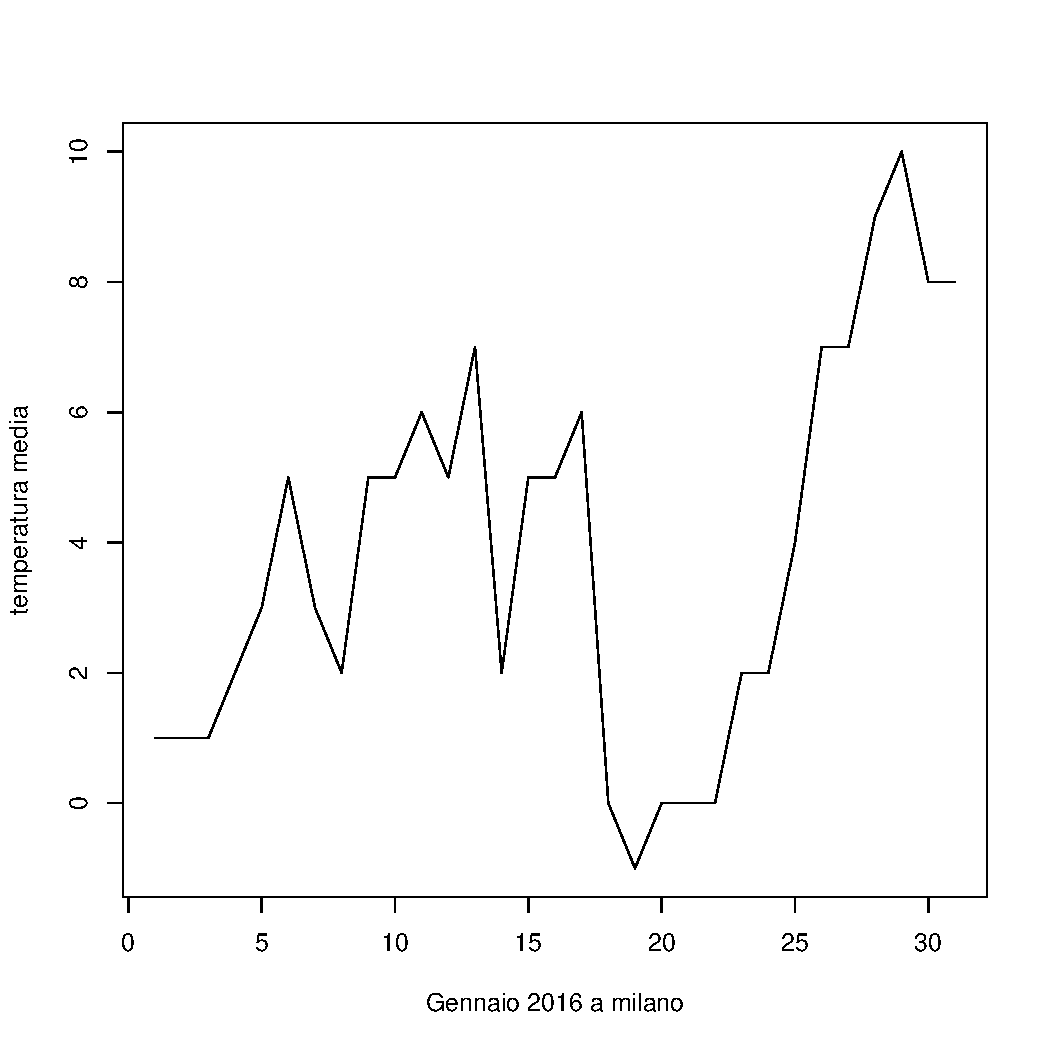
\includegraphics[width=\maxwidth]{figure/unnamed-chunk-56-1} 

\end{knitrout}
\caption{ Andamento della temperatura a Gennaio 2016  a Milano. }
\label{fig:datiist}
\end{center}
\end{figure}

Raggruppiamo ora i dati in classi comprese  tra due estremi che comprendano certamente tutti i dati, per esempio \ensuremath{-2} e 10, decidendo di applicare un passo di 2 e vedere come si distribuiscono. Il comando \texttt{cut} associa a ciascun dato la classe di appartenenza selezionata in base ai punti di taglio.

\begin{knitrout}
\definecolor{shadecolor}{rgb}{0.969, 0.969, 0.969}\color{fgcolor}\begin{kframe}
\begin{alltt}
\hlstd{tagli}\hlkwb{=}\hlkwd{c}\hlstd{(}\hlopt{-}\hlnum{2}\hlstd{,}\hlnum{0}\hlstd{,}\hlnum{2}\hlstd{,}\hlnum{4}\hlstd{,}\hlnum{6}\hlstd{,}\hlnum{10}\hlstd{)}
\hlkwd{cut}\hlstd{(Milano,}\hlkwc{breaks}\hlstd{=tagli)}
\end{alltt}
\begin{verbatim}
##  [1] (0,2]  (0,2]  (0,2]  (0,2]  (2,4]  (4,6]  (2,4]  (0,2] 
##  [9] (4,6]  (4,6]  (4,6]  (4,6]  (6,10] (0,2]  (4,6]  (4,6] 
## [17] (4,6]  (-2,0] (-2,0] (-2,0] (-2,0] (-2,0] (0,2]  (0,2] 
## [25] (2,4]  (6,10] (6,10] (6,10] (6,10] (6,10] (6,10]
## Levels: (-2,0] (0,2] (2,4] (4,6] (6,10]
\end{verbatim}
\end{kframe}
\end{knitrout}

Il comando \texttt{table} conta i dati di ciascuna classe

\begin{knitrout}
\definecolor{shadecolor}{rgb}{0.969, 0.969, 0.969}\color{fgcolor}\begin{kframe}
\begin{alltt}
\hlkwd{table}\hlstd{(}\hlkwd{cut}\hlstd{(Milano,}\hlkwc{breaks}\hlstd{=tagli))}
\end{alltt}
\begin{verbatim}
## 
## (-2,0]  (0,2]  (2,4]  (4,6] (6,10] 
##      5      8      3      8      7
\end{verbatim}
\end{kframe}
\end{knitrout}
Si noti che la suddivisione in classi prevede intervalli aperti a sinistra e chiusi a destra.
Per suddividere in modo che gli intervalli siano chiusi a sinistra e aperti a destra si specifica il parametro \texttt{right=FALSE}.
Possiamo anche usare il comando \texttt{seq} per specificare i tagli.
 \begin{eqnarray*}
\texttt{table(cut}( \varia{variabile},\texttt{breaks=seq}(\varia{estremo inf},\\
\varia{estremo sup},\texttt{by}=\varia{passo}),\texttt{right=TRUE}))
\end{eqnarray*}
o in modo  pi\`u generale
\begin{eqnarray*}
&\texttt{table(cut}(\varia{ variabile},\\
&\texttt{breaks=c}(\varia{estremo\; inferiore}, \ldots,\varia{estremo superiore}))
\end{eqnarray*}
estremamente utile in quanto consente di raggruppare i dati in classi non necessariamente di ugual ampiezza.
\begin{knitrout}
\definecolor{shadecolor}{rgb}{0.969, 0.969, 0.969}\color{fgcolor}\begin{kframe}
\begin{alltt}
\hlkwd{table}\hlstd{(}\hlkwd{cut}\hlstd{(Milano,}\hlkwc{breaks}\hlstd{=}\hlkwd{c}\hlstd{(}\hlopt{-}\hlnum{3}\hlstd{,}\hlnum{1}\hlstd{,}\hlnum{3}\hlstd{,}\hlnum{4}\hlstd{,}\hlnum{5}\hlstd{,}\hlnum{6}\hlstd{,}\hlnum{8}\hlstd{,}\hlnum{10}\hlstd{)))}
\end{alltt}
\begin{verbatim}
## 
## (-3,1]  (1,3]  (3,4]  (4,5]  (5,6]  (6,8] (8,10] 
##      8      7      1      6      2      5      2
\end{verbatim}
\end{kframe}
\end{knitrout}
Volendo raggruppare in classi i dati delle precedenti uscite del dado possiamo scrivere
\begin{knitrout}
\definecolor{shadecolor}{rgb}{0.969, 0.969, 0.969}\color{fgcolor}\begin{kframe}
\begin{alltt}
\hlkwd{table}\hlstd{(}\hlkwd{cut}\hlstd{(dadi100,}\hlkwc{breaks}\hlstd{=}\hlnum{0}\hlopt{:}\hlnum{6}\hlstd{))}
\end{alltt}
\begin{verbatim}
## 
## (0,1] (1,2] (2,3] (3,4] (4,5] (5,6] 
##    15    25    11    17    18    14
\end{verbatim}
\end{kframe}
\end{knitrout}
Se scegliamo di chiudere a sinistra gli intervalli dobbiamo però includere il 7 altrimenti 
il valore 6 non risutlerebbe incluso.
\begin{knitrout}
\definecolor{shadecolor}{rgb}{0.969, 0.969, 0.969}\color{fgcolor}\begin{kframe}
\begin{alltt}
\hlkwd{table}\hlstd{(}\hlkwd{cut}\hlstd{(dadi100,}\hlkwc{breaks}\hlstd{=} \hlnum{1}\hlopt{:}\hlnum{7}\hlstd{,}\hlkwc{right}\hlstd{=}\hlnum{FALSE}\hlstd{))}
\end{alltt}
\begin{verbatim}
## 
## [1,2) [2,3) [3,4) [4,5) [5,6) [6,7) 
##    15    25    11    17    18    14
\end{verbatim}
\end{kframe}
\end{knitrout}

\subsection{Areogrammi}
Il comando generico per generare un istogramma \`e:
\begin{equation*}
\texttt{hist}(\varia{variabile})\index{\texttt{hist}}
\end{equation*}
che segue per\`o la struttura del comando \texttt{cut}. L'ampiezza di ciascuna classe salvo diversamente indicato \`e costante e decisa da \textsf{R}.
\`E  possibile variare tale condizione definendo una lista con i punti di taglio ({\it cutoff}) delle classi volute:
\begin{equation} \texttt{hist}(\varia{variabile},\texttt{c}(\varia{valore}_1, \varia{valore}_2, \ldots))
\end{equation}
Per esempio se \texttt{dadi100} rappresenta le solite 100 uscite del lancio del dado, il comando
\begin{knitrout}
\definecolor{shadecolor}{rgb}{0.969, 0.969, 0.969}\color{fgcolor}\begin{kframe}
\begin{alltt}
\hlkwd{par}\hlstd{(}\hlkwc{mfrow}\hlstd{=}\hlkwd{c}\hlstd{(}\hlnum{1}\hlstd{,}\hlnum{2}\hlstd{))}
\hlkwd{hist}\hlstd{(dadi100,}\hlkwc{breaks}\hlstd{=}\hlkwd{seq}\hlstd{(}\hlnum{0.5}\hlstd{,}\hlnum{6.5}\hlstd{,}\hlnum{1}\hlstd{),}\hlkwc{col}\hlstd{=}\hlstr{"red"}\hlstd{)}
\hlkwd{hist}\hlstd{(dadi100,}\hlkwc{freq}\hlstd{=}\hlnum{FALSE}\hlstd{,}\hlkwc{breaks}\hlstd{=}\hlkwd{seq}\hlstd{(}\hlnum{0.5}\hlstd{,}\hlnum{6.5}\hlstd{,}\hlnum{1}\hlstd{),}\hlkwc{col}\hlstd{=}\hlstr{"blue"}\hlstd{)}
\end{alltt}
\end{kframe}
\end{knitrout}
\begin{figure}[htbp]
\begin{center}
\begin{knitrout}
\definecolor{shadecolor}{rgb}{0.969, 0.969, 0.969}\color{fgcolor}
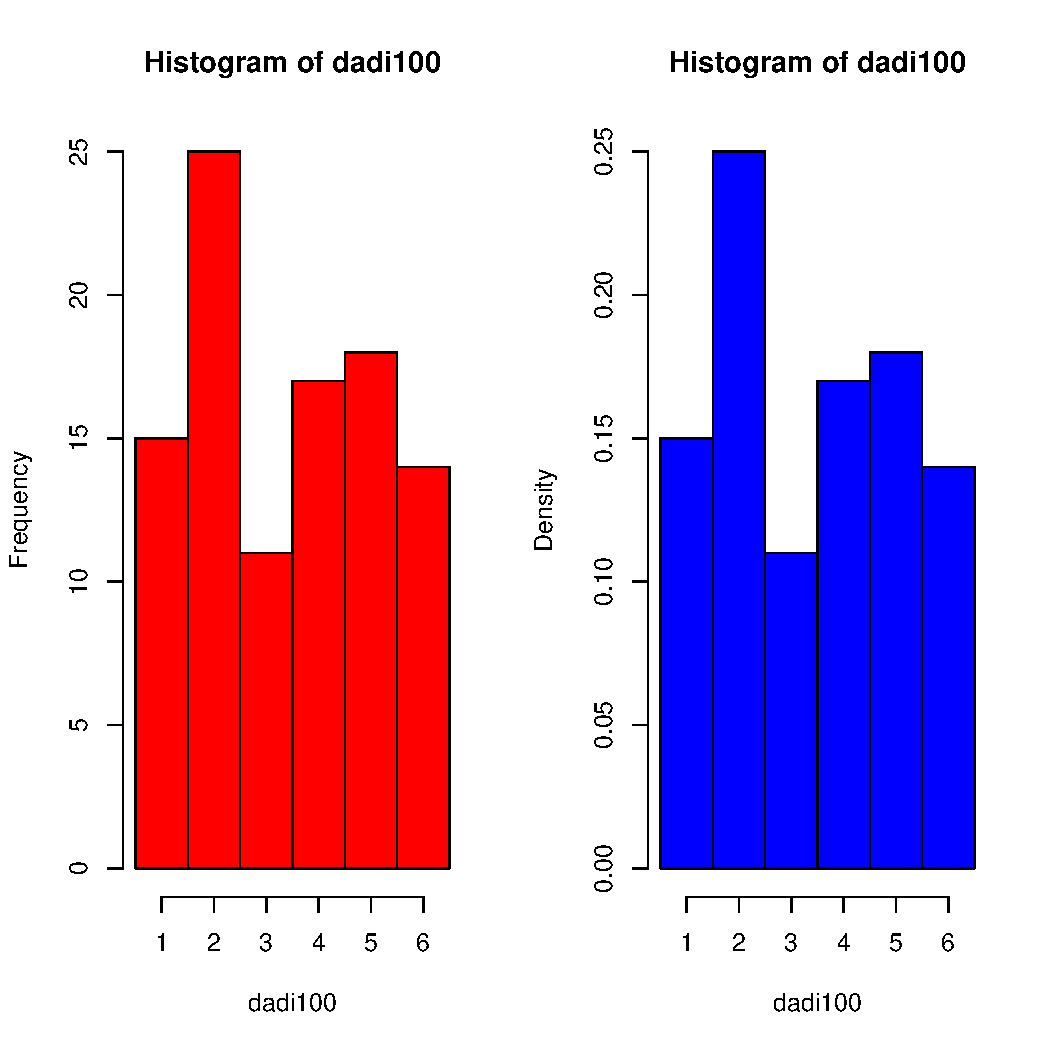
\includegraphics[width=\maxwidth]{figure/unnamed-chunk-63-1} 

\end{knitrout}
\caption{Diagramma a colonne e areogramma per il lancio di un dado.}
\label{fig:datidado}
\end{center}
\end{figure}
genera l'istogramma (in rosso, a sinistra Figura~\ref{fig:datiist}) con le frequenze assolute delle classi in ordinata. La sequenza dei punti di taglio \`e stata scelta in modo che i numeri interi da 1 a 6 siano al centro delle classi corrispondenti. Se invece volessimo creare un areogramma  (ossia avere un tracciato per cui le aree siano pari alle frequenze relative) a partire dalle stesse uscite dovremo imporre il parametro \texttt{freq=FALSE} otterremo il pannello a destra (in blu) della figura~(\ref{fig:datiist}). Avendo scelto classi di ampiezza costante i 2 grafici differiscono semplicemente per un cambio di scala sull'asse $y$.

In modo simile possiamo tracciare un areogramma  dei dati nella variabile \texttt{milano}
\begin{knitrout}
\definecolor{shadecolor}{rgb}{0.969, 0.969, 0.969}\color{fgcolor}\begin{kframe}
\begin{alltt}
\hlkwd{par}\hlstd{(}\hlkwc{mfrow}\hlstd{=}\hlkwd{c}\hlstd{(}\hlnum{1}\hlstd{,}\hlnum{2}\hlstd{))}
\hlkwd{hist}\hlstd{(Milano,} \hlkwc{col}\hlstd{=}\hlstr{"green"}\hlstd{,}\hlkwc{freq}\hlstd{=}\hlnum{FALSE}\hlstd{,}\hlkwc{right}\hlstd{=}\hlnum{FALSE}\hlstd{,}
\hlkwc{main}\hlstd{=}\hlstr{"Cutoff automatici"}\hlstd{)}
\end{alltt}
\end{kframe}
\end{knitrout}
lasciando \textsf{R} libero di scegliere i punti di taglio (pannelli a sinistra della figura \ref{fig:datiistmilano}) o scegliendoli a nostra volta (pannelli a destra della stessa figura  \ref{fig:datiistmilano})

\begin{knitrout}
\definecolor{shadecolor}{rgb}{0.969, 0.969, 0.969}\color{fgcolor}\begin{kframe}
\begin{alltt}
\hlkwd{hist}\hlstd{(Milano,}\hlkwc{col}\hlstd{=}\hlstr{"red"}\hlstd{,}\hlkwc{freq}\hlstd{=}\hlnum{FALSE}\hlstd{,}
\hlkwc{breaks}\hlstd{=}\hlkwd{unique}\hlstd{(}\hlkwd{as.vector}\hlstd{(}\hlkwd{quantile}\hlstd{(Milano,}\hlkwd{seq}\hlstd{(}\hlnum{0}\hlstd{,}\hlnum{1}\hlstd{,}\hlkwc{by}\hlstd{=}\hlnum{1}\hlopt{/}\hlnum{6}\hlstd{)))),}
\hlkwc{main}\hlstd{=}\hlstr{"Cutoff personalizzati"}\hlstd{)}
\end{alltt}
\end{kframe}
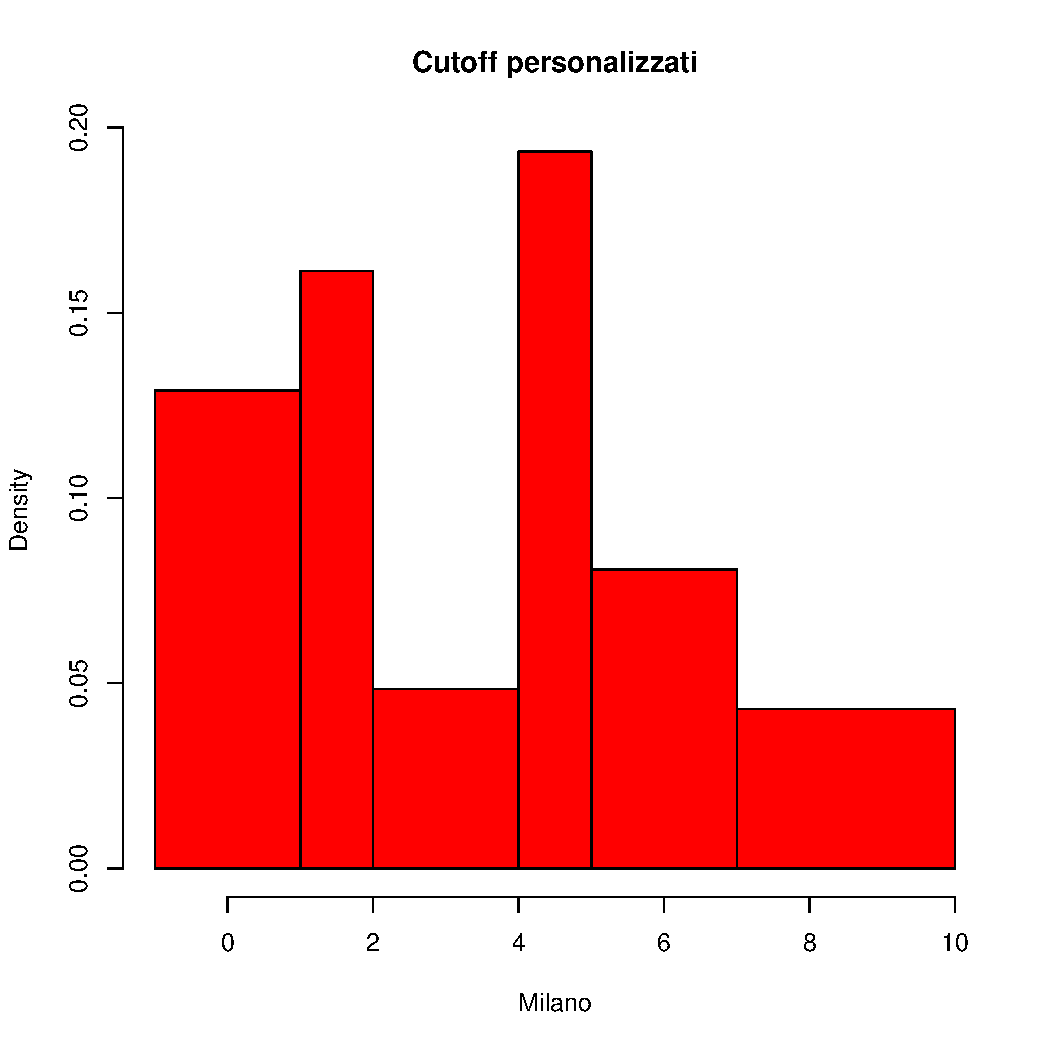
\includegraphics[width=\maxwidth]{figure/unnamed-chunk-66-1} 

\end{knitrout}
\begin{figure}[htbp]
\begin{center}
\begin{knitrout}
\definecolor{shadecolor}{rgb}{0.969, 0.969, 0.969}\color{fgcolor}
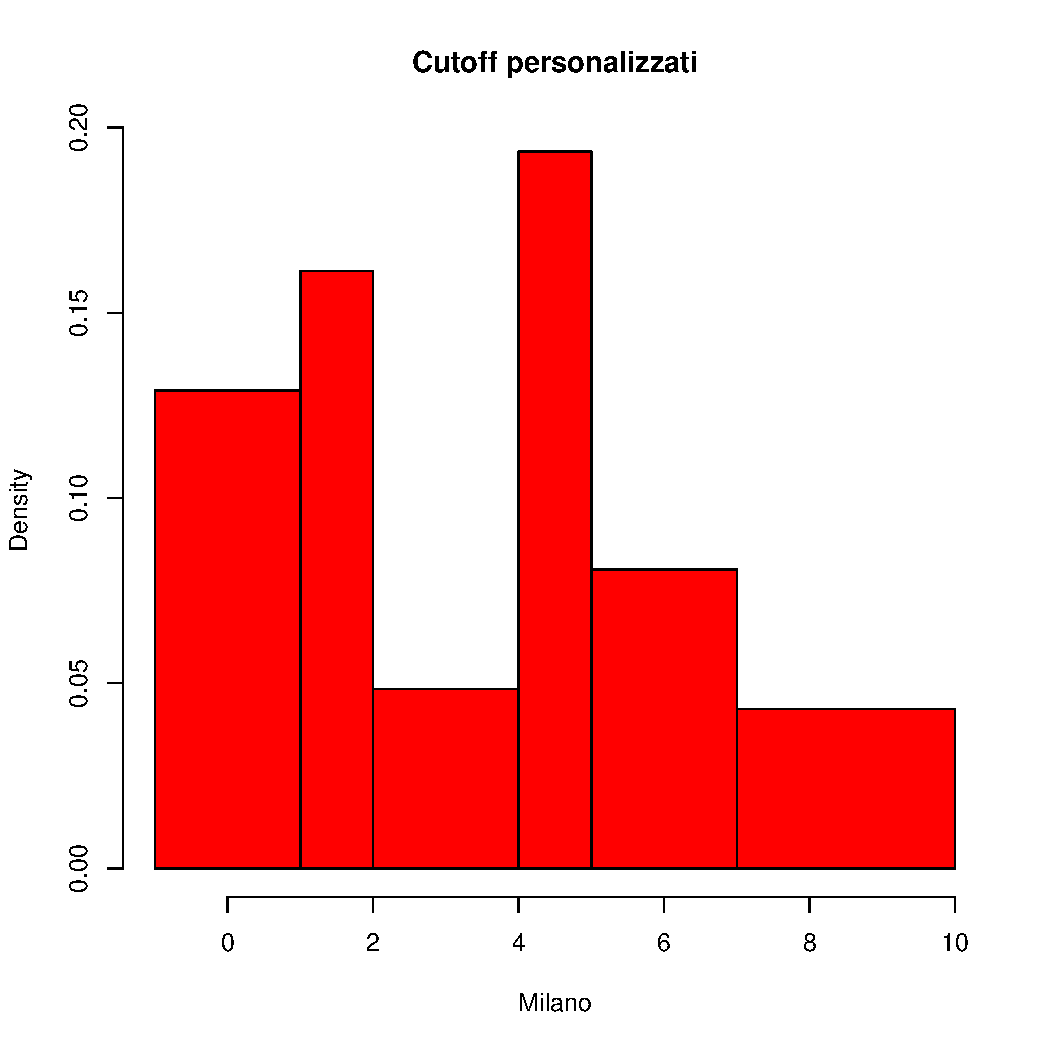
\includegraphics[width=\maxwidth]{figure/unnamed-chunk-67-1} 

\end{knitrout}
\caption{ Areogramma dei dati della temperatura. Scelta automatica dei punti di taglio.}
\label{fig:datiistmilano}
\end{center}
\end{figure}
Si noti la stabilit\`a degli areogrammi rispetto ai cambi nella suddivisione.
\subsection{Generazione di boxplot}

Il \texttt{boxplot}  \`e una rappresentazione grafica immediata della statistica dei 5 numeri e simultaneamente ci  segnala eventuali punti discordanti o anomali, {\it outlier}.
Il comando generico \`e: \begin{equation}\texttt{boxplot}(\varia{variabile})\end{equation}
prendendo il vettore $x$ contenente i risultati di 100 lanci
otteniamo la figura~\ref{fig:boxplotdado}
\begin{figure}[htbp]
\begin{center}
\begin{knitrout}
\definecolor{shadecolor}{rgb}{0.969, 0.969, 0.969}\color{fgcolor}\begin{kframe}
\begin{alltt}
\hlkwd{boxplot}\hlstd{(dadi100)}
\end{alltt}
\end{kframe}
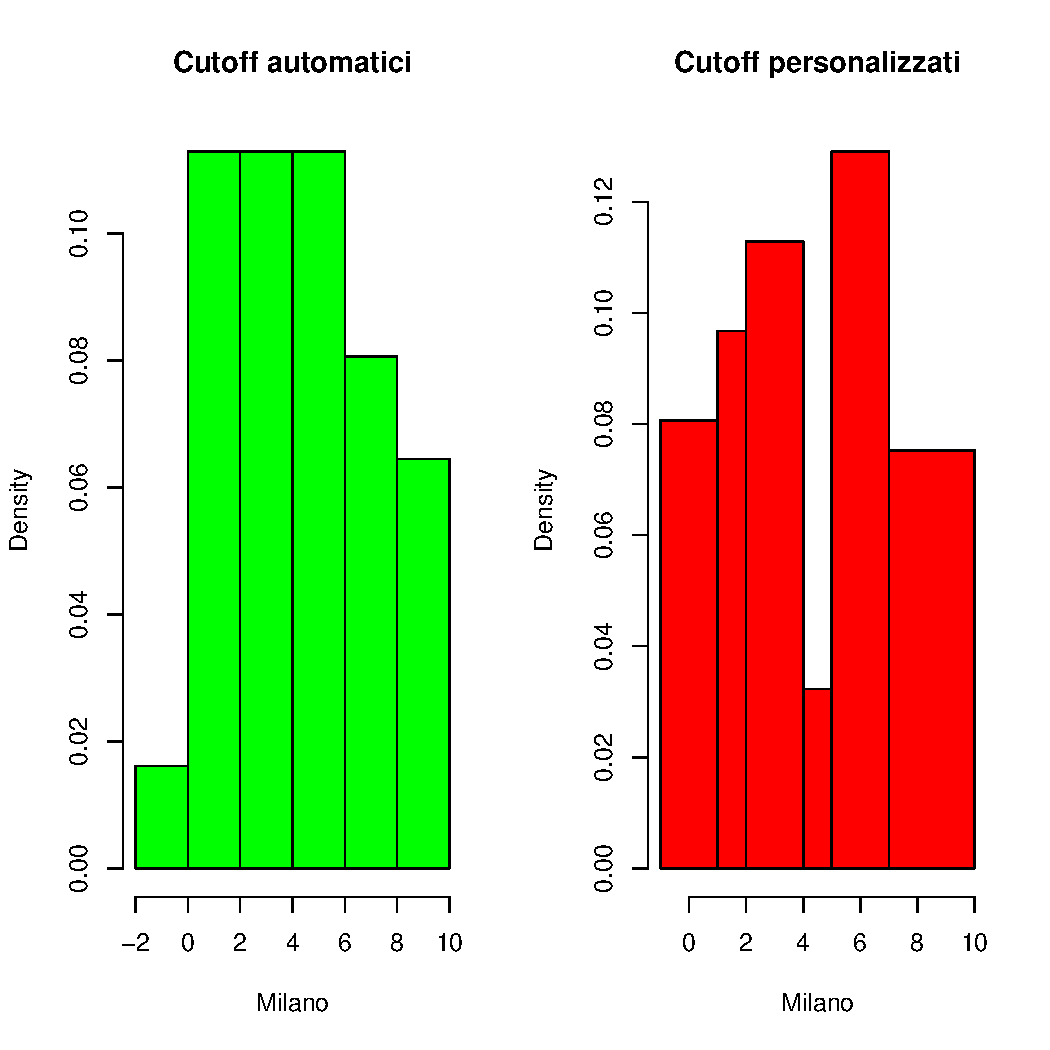
\includegraphics[width=\maxwidth]{figure/unnamed-chunk-68-1} 

\end{knitrout}
\caption{Boxplot dei risultati del lancio di un dado}
\label{fig:boxplotdado}
\end{center}
\end{figure}
da cui si evince che il valore massimo dei dati \`e 6, il minimo \`e 1 e non ci sono punti anomali, per cui non vi sono dati anomali, altrimenti evidenziati da un pallino. Si legge inoltre il valore di mediana (4) primo quartile (2) e terzo quartile (5).

\subsection{Creazione di grafici a torta}

Il comando \texttt{pie} consente, partendo da una tabella, di tracciare il diagramma a torta per una variabile nominale raggruppata in classi. Il comando \`e

\begin{equation*}\texttt{pie(table}(\varia{variabile} ))
\end{equation*}
ad esempio (facendo riferimento ai precedenti dati):
\begin{knitrout}
\definecolor{shadecolor}{rgb}{0.969, 0.969, 0.969}\color{fgcolor}\begin{kframe}
\begin{alltt}
\hlkwd{pie}\hlstd{(}\hlkwd{table}\hlstd{(dadi100))}
\end{alltt}
\end{kframe}
\end{knitrout}
fornisce in uscita  la Figura~\ref{fig:pie}
\begin{figure}[htbp]
\begin{center}
\begin{knitrout}
\definecolor{shadecolor}{rgb}{0.969, 0.969, 0.969}\color{fgcolor}
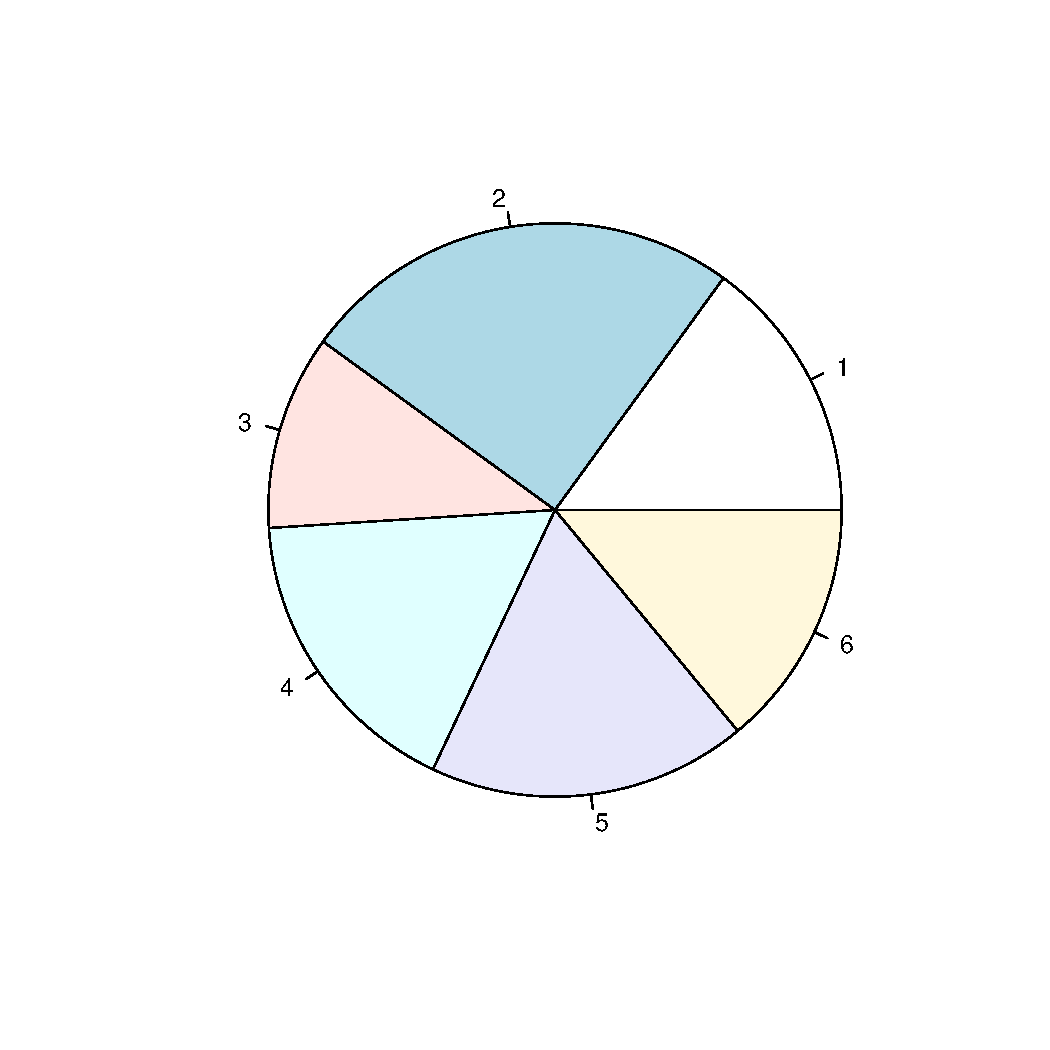
\includegraphics[width=\maxwidth]{figure/unnamed-chunk-70-1} 

\end{knitrout}
\caption{Diagramma a torta per il lancio di un dado equo.}
\label{fig:pie}
\end{center}
\end{figure}
\begin{shaded}{Costruire una matrice contenente le coordinate di 50 punti nel rettangolo $[0,4]\times [0,2]$ in due dimensioni (generate utilizzando il generatore di numeri pseudocasuali). Produrre un grafico con due pannelli, dove il primo pannello \`e uno scatter-plot}
\end{shaded}
\section{Variabili doppie e rette di regressione}
Supponiamo di misurare la concentrazione di acido lattico muscolare durante uno sforzo di 10 minuti,
\begin{knitrout}
\definecolor{shadecolor}{rgb}{0.969, 0.969, 0.969}\color{fgcolor}\begin{kframe}
\begin{alltt}
\hlstd{x}\hlkwb{<-}\hlstd{tempo}\hlkwb{<-}\hlkwd{c}\hlstd{(}\hlnum{1}\hlstd{,}\hlnum{2}\hlstd{,}\hlnum{3}\hlstd{,}\hlnum{4}\hlstd{,}\hlnum{5}\hlstd{,}\hlnum{6}\hlstd{,}\hlnum{7}\hlstd{,}\hlnum{8}\hlstd{,}\hlnum{9}\hlstd{,}\hlnum{10}\hlstd{)}
\hlstd{y}\hlkwb{<-}\hlstd{concentrazione}\hlkwb{<-}\hlkwd{c}\hlstd{(}\hlnum{0.3}\hlstd{,}\hlnum{0.65}\hlstd{,}\hlnum{0.7}\hlstd{,}\hlnum{0.8}\hlstd{,}\hlnum{0.95}\hlstd{,}\hlnum{1.05}\hlstd{,}\hlnum{1.3}\hlstd{,}\hlnum{1.7}\hlstd{,}\hlnum{1.9}\hlstd{,}
\hlnum{2.5}\hlstd{)}
\end{alltt}
\end{kframe}
\end{knitrout}
Per analizzare questi dati conviene preliminarmente tracciarne un diagramma a dispersione.
\begin{figure}[htbp]
\begin{center}
\begin{knitrout}
\definecolor{shadecolor}{rgb}{0.969, 0.969, 0.969}\color{fgcolor}\begin{kframe}
\begin{alltt}
\hlkwd{plot}\hlstd{(x,y)}
\end{alltt}
\end{kframe}
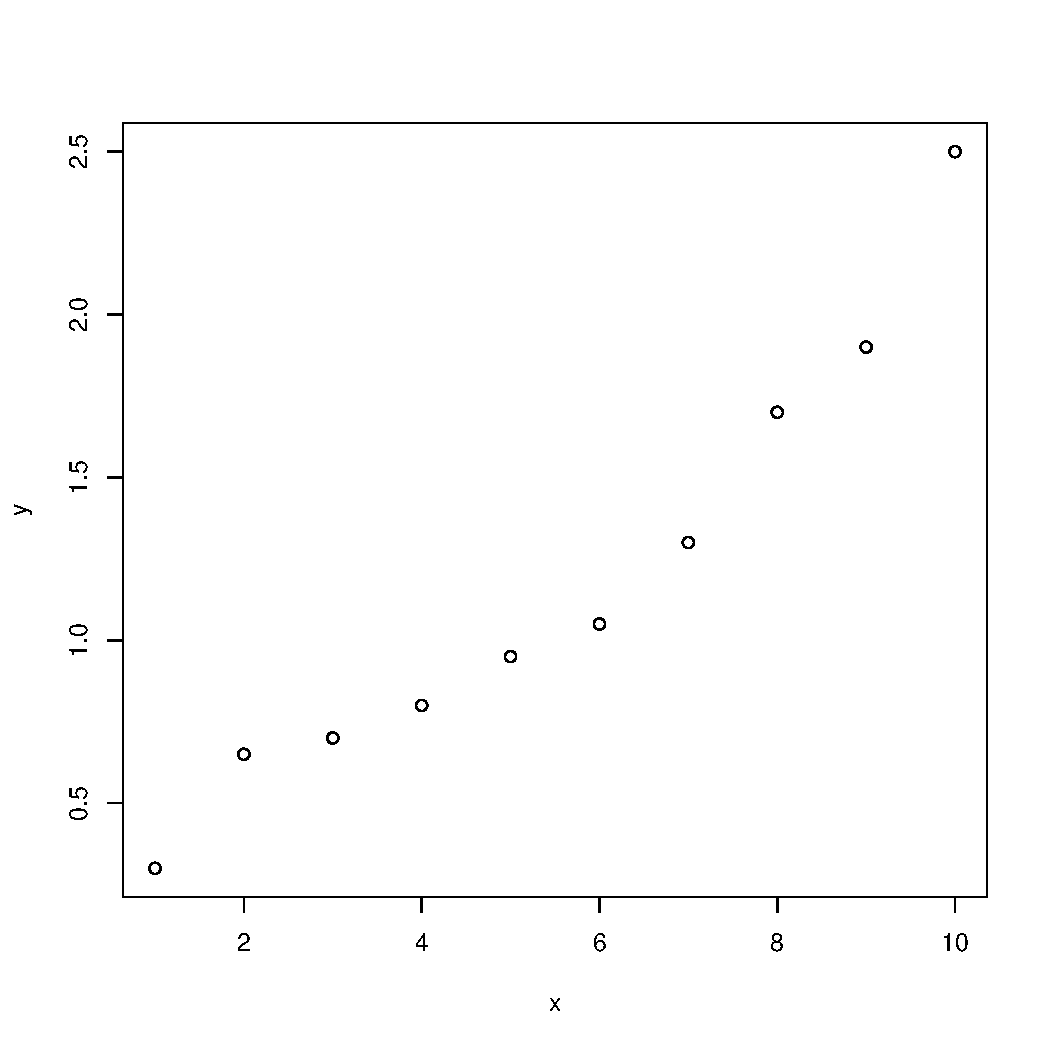
\includegraphics[width=\maxwidth]{figure/unnamed-chunk-72-1} 

\end{knitrout}
\caption{Diagramma a dispersione tempo/concentrazione.}
\label{fig:scatte}
\end{center}
\end{figure}
Possiamo inoltre determinare il coefficiente di correlazione lineare
\begin{knitrout}
\definecolor{shadecolor}{rgb}{0.969, 0.969, 0.969}\color{fgcolor}\begin{kframe}
\begin{alltt}
\hlkwd{cor}\hlstd{(x,y)}
\end{alltt}
\begin{verbatim}
## [1] 0.9620456
\end{verbatim}
\end{kframe}
\end{knitrout}
Per definire un modello di relazione lineare occorre usare il comando \texttt{lm} (\varia{linear model}).
Nella sua generica forma il comando \`e espresso come\footnote{ Per digitare la tilde  \mytilde\;  su Mac premere ALT 5 su PC invece il tasto Alt Gr (attivazione del codice ASCII) e sul tastierino numerico digitare il numero 126. Lavorando su un portatile il tastierino numerico \`e spesso incorporato nella tastiera con colorazione blu dei tasti.}
$$\texttt{lm}(\varia{y} \sim  \varia{x})$$
Otteniamo i valori di pendenza e intercetta.

Possiamo tracciare la retta di regressione con il comando \texttt{abline}.
\begin{knitrout}
\definecolor{shadecolor}{rgb}{0.969, 0.969, 0.969}\color{fgcolor}\begin{kframe}
\begin{alltt}
\hlkwd{plot}\hlstd{(x,y,}\hlkwc{pch}\hlstd{=}\hlnum{19}\hlstd{,}\hlkwc{col}\hlstd{=}\hlstr{"red"}\hlstd{)}
\hlkwd{abline}\hlstd{(}\hlkwd{lm}\hlstd{(y}\hlopt{~}\hlstd{x),}\hlkwc{col}\hlstd{=}\hlstr{"blue"}\hlstd{)}
\end{alltt}
\end{kframe}
\end{knitrout}
Per determinare  la retta di regressione sulle $y$ dobbiamo invertire $x$ e $y$.
\begin{knitrout}
\definecolor{shadecolor}{rgb}{0.969, 0.969, 0.969}\color{fgcolor}\begin{kframe}
\begin{alltt}
\hlstd{(modellox}\hlkwb{=}\hlkwd{lm}\hlstd{(x}\hlopt{~}\hlstd{y))}
\end{alltt}
\begin{verbatim}
## 
## Call:
## lm(formula = x ~ y)
## 
## Coefficients:
## (Intercept)            y  
##      0.3516       4.3446
\end{verbatim}
\begin{alltt}
\hlstd{coeff}\hlkwb{=}\hlstd{modellox}\hlopt{$}\hlstd{coefficients}
\hlstd{(a}\hlkwb{=}\hlnum{1}\hlopt{/}\hlstd{coeff[}\hlnum{2}\hlstd{])}
\end{alltt}
\begin{verbatim}
##         y 
## 0.2301707
\end{verbatim}
\begin{alltt}
\hlstd{(b}\hlkwb{=}\hlopt{-}\hlstd{coeff[}\hlnum{1}\hlstd{]}\hlopt{/}\hlstd{coeff[}\hlnum{2}\hlstd{])}
\end{alltt}
\begin{verbatim}
## (Intercept) 
## -0.08093883
\end{verbatim}
\begin{alltt}
\hlkwd{abline}\hlstd{(b,a,}\hlkwc{col}\hlstd{=}\hlstr{"green"}\hlstd{)}
\end{alltt}


{\ttfamily\noindent\bfseries\color{errorcolor}{\#\# Error in int\_abline(a = a, b = b, h = h, v = v, untf = untf, ...): plot.new has not been called yet}}\end{kframe}
\end{knitrout}
In tal modo otteniamo il grafico~\ref{fig:duerettex}.
\begin{center}
\begin{figure}[htbp]
\begin{knitrout}
\definecolor{shadecolor}{rgb}{0.969, 0.969, 0.969}\color{fgcolor}
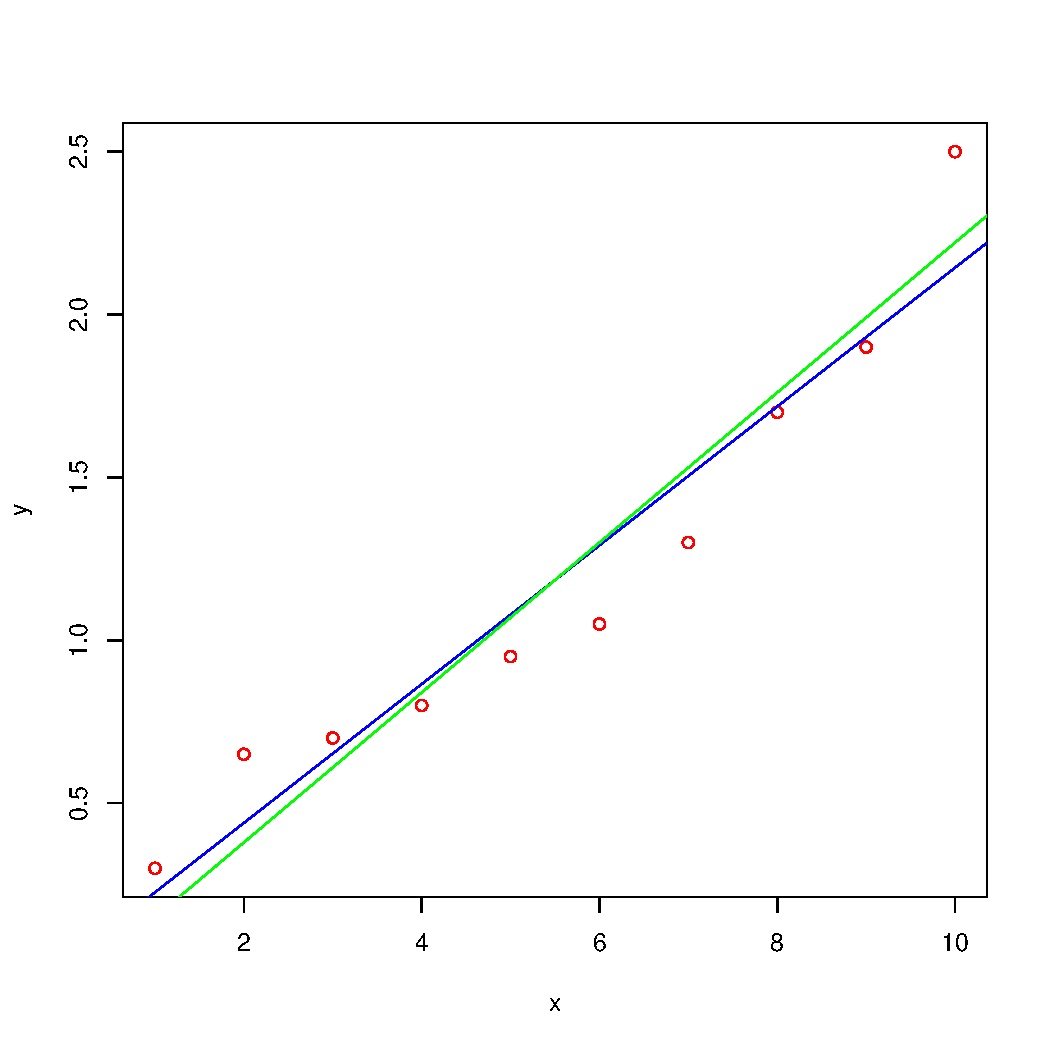
\includegraphics[width=\maxwidth]{figure/unnamed-chunk-76-1} 

\end{knitrout}
\caption{Rette di regressione. In blu $R_x$, in verde $R_y$.}
\label{fig:duerettex}
\end{figure}
\end{center}

\subsubsection{I bambini di Kalama (Egitto). Ancora retta di regressione}
Da DASL \cite{DASL} possiamo scaricare un \emph{dataset} in cui i ricercatori hanno misurato le altezze (cm) dai 18 ai 29 mesi di vita, di 161 bambini di Kalama, un villaggio egiziano. Le altezze sono state mediate tra i bambini per fornire un singolo valore mese per mese.
\begin{knitrout}
\definecolor{shadecolor}{rgb}{0.969, 0.969, 0.969}\color{fgcolor}\begin{kframe}
\begin{alltt}
\hlstd{age}\hlkwb{=}\hlnum{18}\hlopt{:}\hlnum{29}
\hlstd{height}\hlkwb{=}\hlkwd{c}\hlstd{(}\hlnum{76.1}\hlstd{,}\hlnum{77}\hlstd{,}\hlnum{78.1}\hlstd{,}\hlnum{78.2}\hlstd{,}\hlnum{78.8}\hlstd{,}\hlnum{79.7}\hlstd{,}\hlnum{79.9}\hlstd{,}\hlnum{81.1}\hlstd{,}\hlnum{81.2}\hlstd{,}\hlnum{81.8}\hlstd{,}\hlnum{82.8}\hlstd{,}\hlnum{83.5}\hlstd{)}
\end{alltt}
\end{kframe}
\end{knitrout}
Possiamo quindi costruire il \texttt{data.frame}
\begin{knitrout}
\definecolor{shadecolor}{rgb}{0.969, 0.969, 0.969}\color{fgcolor}\begin{kframe}
\begin{alltt}
\hlstd{village}\hlkwb{=}\hlkwd{data.frame}\hlstd{(}\hlkwc{age}\hlstd{=age,}\hlkwc{height}\hlstd{=height)}
\end{alltt}
\end{kframe}
\end{knitrout}
Ora diamo una prima occhiata ai dati:
 %code chunk
\begin{figure}[htbp]
\begin{center}
\begin{knitrout}
\definecolor{shadecolor}{rgb}{0.969, 0.969, 0.969}\color{fgcolor}\begin{kframe}
\begin{alltt}
\hlkwd{plot}\hlstd{(age,height)}
\end{alltt}
\end{kframe}
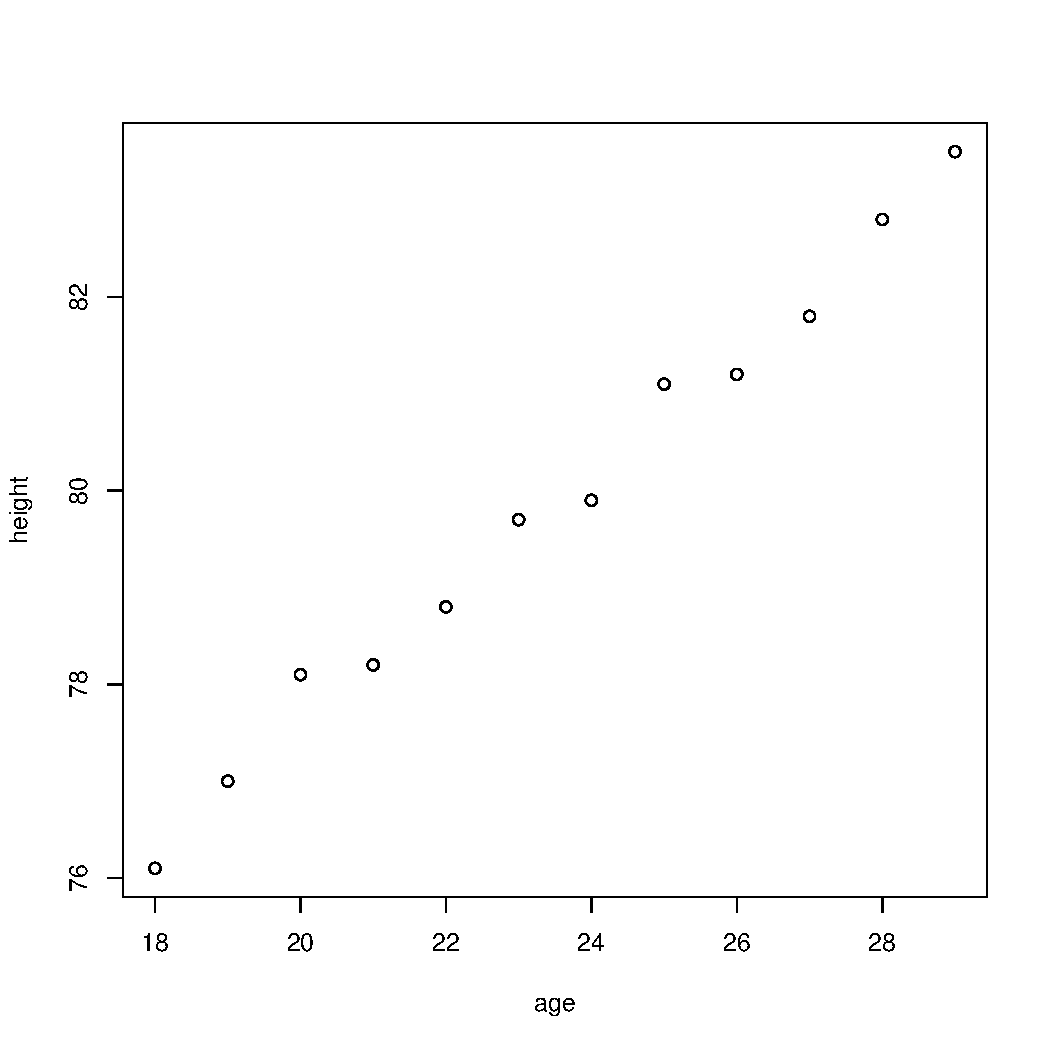
\includegraphics[width=\maxwidth]{figure/unnamed-chunk-79-1} 

\end{knitrout}
\caption{Crescita dei bambini di Kalama}
\label{kalama}
\end{center}
\end{figure}
L'andamento \`e lineare. Determiniamo la retta di regressione
per predire l'altezza media nota l'et\`a in mesi.
%code chunk
\begin{knitrout}
\definecolor{shadecolor}{rgb}{0.969, 0.969, 0.969}\color{fgcolor}\begin{kframe}
\begin{alltt}
\hlstd{(modello}\hlkwb{=}\hlkwd{lm}\hlstd{(height}\hlopt{~}\hlstd{age))}
\end{alltt}
\begin{verbatim}
## 
## Call:
## lm(formula = height ~ age)
## 
## Coefficients:
## (Intercept)          age  
##      64.928        0.635
\end{verbatim}
\end{kframe}
\end{knitrout}
La retta di regressione cercata ha formula:
$$h(\texttt{age})=64.93+ 0.63\, \texttt{age}$$

Possiamo ora utilizzare \textsf{R} come semplice calcolatore per predire l'altezza a 27.5 mesi di et\`a:
oppure, \`e pi\`u  efficiente utilizzare direttamente il \emph{dataframe} e la funzione
\texttt{predict}:
%codechunk
\begin{knitrout}
\definecolor{shadecolor}{rgb}{0.969, 0.969, 0.969}\color{fgcolor}\begin{kframe}
\begin{alltt}
\hlkwd{predict}\hlstd{(modello,}\hlkwd{data.frame}\hlstd{(}\hlkwc{age}\hlstd{=}\hlnum{27.5}\hlstd{))}
\end{alltt}
\begin{verbatim}
##        1 
## 82.38986
\end{verbatim}
\end{kframe}
\end{knitrout}
fornendo in input i parametri della retta ed un preciso valore della variabile indipendente (richiamata col proprio nome).
Molti comandi di \textsf{R} sono in grado di manipolare \emph{dataframe}  lavorando direttamente sulla struttura. Per esempio, il comando plot di un \texttt{dataframe} in due colonne, esegue in automatico il grafico della seconda colonna (variabile dipendente) vs prima colonna (variabile indipendente).
Possiamo ottenere il modello lineare visto nel caso precedente, passando \texttt{village} direttamente al comando:
\begin{knitrout}
\definecolor{shadecolor}{rgb}{0.969, 0.969, 0.969}\color{fgcolor}\begin{kframe}
\begin{alltt}
\hlstd{modello}\hlkwb{=}\hlkwd{lm}\hlstd{(height}\hlopt{~}\hlstd{age,}\hlkwc{data}\hlstd{=village)}
\hlstd{modello}
\end{alltt}
\begin{verbatim}
## 
## Call:
## lm(formula = height ~ age, data = village)
## 
## Coefficients:
## (Intercept)          age  
##      64.928        0.635
\end{verbatim}
\end{kframe}
\end{knitrout}
con la formula \texttt{lm(y \mytilde x,data=dataset)}.
%Inoltre possiamo considerare il plot di un oggetto \texttt{lm}  che fornisce una serie di rappresentazioni grafiche
%<<fig=TRUE,echo=FALSE>>=
%oldpar<-par(mfrow=c(2,2))
%par(ask=FALSE)
%plot(lm(height~age))
%oldpar
%@
\section{Modelli potenza}
Consideriamo ora il seguente \emph{dataset} di mammiferi  in cui le 2 variabili rappresentano  le dimensioni del corpo e del cervello.
\begin{knitrout}
\definecolor{shadecolor}{rgb}{0.969, 0.969, 0.969}\color{fgcolor}\begin{kframe}
\begin{alltt}
\hlkwd{library}\hlstd{(MASS)}
\hlstd{mammals}
\end{alltt}
\begin{verbatim}
##                               body   brain
## Arctic fox                   3.385   44.50
## Owl monkey                   0.480   15.50
## Mountain beaver              1.350    8.10
## Cow                        465.000  423.00
## Grey wolf                   36.330  119.50
## Goat                        27.660  115.00
## Roe deer                    14.830   98.20
## Guinea pig                   1.040    5.50
## Verbet                       4.190   58.00
## Chinchilla                   0.425    6.40
## Ground squirrel              0.101    4.00
## Arctic ground squirrel       0.920    5.70
## African giant pouched rat    1.000    6.60
## Lesser short-tailed shrew    0.005    0.14
## Star-nosed mole              0.060    1.00
## Nine-banded armadillo        3.500   10.80
## Tree hyrax                   2.000   12.30
## N.A. opossum                 1.700    6.30
## Asian elephant            2547.000 4603.00
## Big brown bat                0.023    0.30
## Donkey                     187.100  419.00
## Horse                      521.000  655.00
## European hedgehog            0.785    3.50
## Patas monkey                10.000  115.00
## Cat                          3.300   25.60
## Galago                       0.200    5.00
## Genet                        1.410   17.50
## Giraffe                    529.000  680.00
## Gorilla                    207.000  406.00
## Grey seal                   85.000  325.00
## Rock hyrax-a                 0.750   12.30
## Human                       62.000 1320.00
## African elephant          6654.000 5712.00
## Water opossum                3.500    3.90
## Rhesus monkey                6.800  179.00
## Kangaroo                    35.000   56.00
## Yellow-bellied marmot        4.050   17.00
## Golden hamster               0.120    1.00
## Mouse                        0.023    0.40
## Little brown bat             0.010    0.25
## Slow loris                   1.400   12.50
## Okapi                      250.000  490.00
## Rabbit                       2.500   12.10
## Sheep                       55.500  175.00
## Jaguar                     100.000  157.00
## Chimpanzee                  52.160  440.00
## Baboon                      10.550  179.50
## Desert hedgehog              0.550    2.40
## Giant armadillo             60.000   81.00
## Rock hyrax-b                 3.600   21.00
## Raccoon                      4.288   39.20
## Rat                          0.280    1.90
## E. American mole             0.075    1.20
## Mole rat                     0.122    3.00
## Musk shrew                   0.048    0.33
## Pig                        192.000  180.00
## Echidna                      3.000   25.00
## Brazilian tapir            160.000  169.00
## Tenrec                       0.900    2.60
## Phalanger                    1.620   11.40
## Tree shrew                   0.104    2.50
## Red fox                      4.235   50.40
\end{verbatim}
\end{kframe}
\end{knitrout}
Per prima cosa tracciamo il grafico dei punti  in scala non trasformata e, visto la compresenza di dati molto prossimi all'origine e di dati molto distanti in scala logaritmica (sia le $x$ che le $y$ vengono trasformate prendendone i logaritmi)
\begin{knitrout}
\definecolor{shadecolor}{rgb}{0.969, 0.969, 0.969}\color{fgcolor}\begin{kframe}
\begin{alltt}
\hlkwd{par}\hlstd{(}\hlkwc{mfrow}\hlstd{=}\hlkwd{c}\hlstd{(}\hlnum{1}\hlstd{,}\hlnum{2}\hlstd{))}
\hlkwd{plot}\hlstd{(mammals)}
\hlkwd{plot}\hlstd{(mammals,}\hlkwc{log}\hlstd{=}\hlstr{"xy"}\hlstd{)}
\end{alltt}
\end{kframe}
\end{knitrout}
come in Figura~\ref{fig:duemammals}.\begin{figure}[htbp]
\begin{center}
\begin{knitrout}
\definecolor{shadecolor}{rgb}{0.969, 0.969, 0.969}\color{fgcolor}
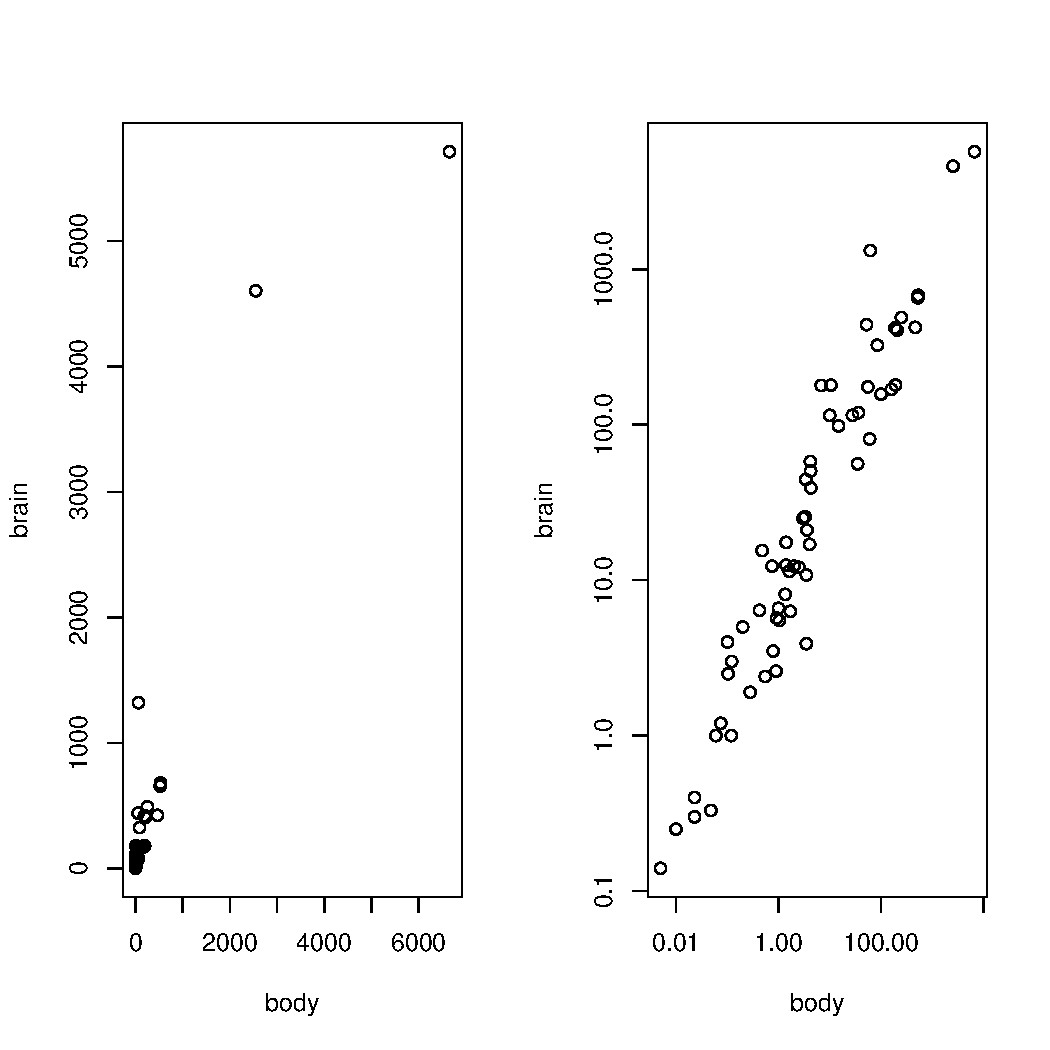
\includegraphics[width=\maxwidth]{figure/unnamed-chunk-85-1} 

\end{knitrout}
\caption{Diagramma a dispersione massa corporea/massa del cervello in scala normale ed in scala logaritmica. }
\label{fig:duemammals}
\end{center}
\end{figure}
Visti i  risultati ottenuti usando la scala logaritmica tracciamo anche la corrispondente retta di regressione
\begin{knitrout}
\definecolor{shadecolor}{rgb}{0.969, 0.969, 0.969}\color{fgcolor}\begin{kframe}
\begin{alltt}
\hlkwd{plot}\hlstd{(}\hlkwd{log}\hlstd{(mammals}\hlopt{$}\hlstd{brain)}\hlopt{~}\hlkwd{log}\hlstd{(mammals}\hlopt{$}\hlstd{body),}\hlkwc{col}\hlstd{=}\hlstr{"BLUE"}\hlstd{,}\hlkwc{pch}\hlstd{=}\hlnum{19}\hlstd{,}\hlkwc{type}\hlstd{=}\hlstr{"p"}\hlstd{)}
\hlkwd{abline}\hlstd{(}\hlkwd{lm}\hlstd{(}\hlkwd{log}\hlstd{(mammals}\hlopt{$}\hlstd{brain)}\hlopt{~} \hlkwd{log}\hlstd{(mammals}\hlopt{$}\hlstd{body)),}\hlkwc{col}\hlstd{=}\hlstr{"red"}\hlstd{,}\hlkwc{lwd}\hlstd{=}\hlnum{3}\hlstd{);}
\hlstd{uomo}\hlkwb{=}\hlkwd{which}\hlstd{(}\hlkwd{rownames}\hlstd{(mammals)}\hlopt{==}\hlstr{"Human"}\hlstd{)}
\hlkwd{text}\hlstd{(}\hlkwd{log}\hlstd{(mammals[uomo ,}\hlnum{1}\hlstd{]),}\hlkwd{log}\hlstd{(mammals[uomo ,}\hlnum{2}\hlstd{]),}\hlkwd{rownames}\hlstd{(mammals)[uomo])}
\end{alltt}
\end{kframe}
\end{knitrout}
\begin{figure}[htbp]
\begin{center}
\begin{knitrout}
\definecolor{shadecolor}{rgb}{0.969, 0.969, 0.969}\color{fgcolor}
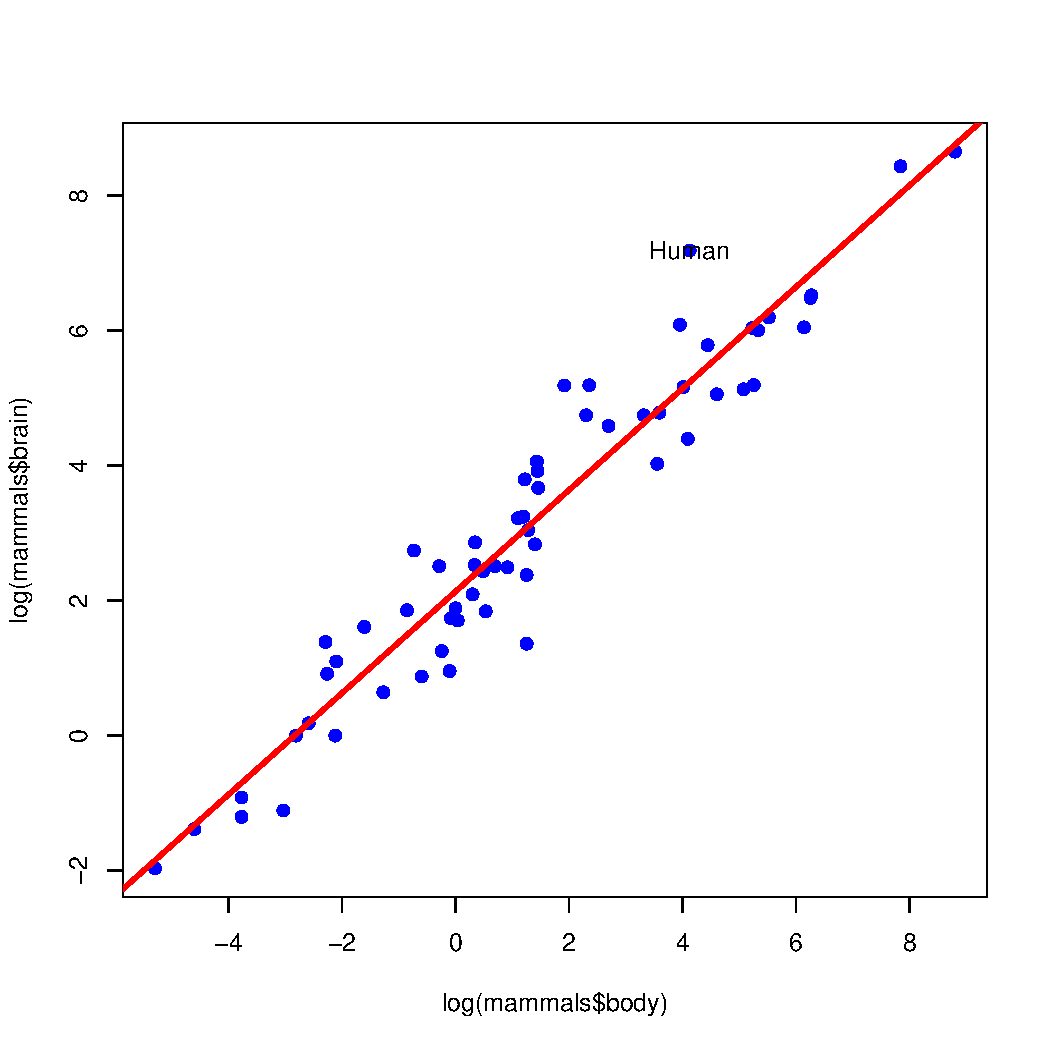
\includegraphics[width=\maxwidth]{figure/unnamed-chunk-87-1} 

\end{knitrout}
\caption{ Retta di regressione. Dimensione del corpo e del cervello. Si noti la posizione dell'uomo.}
\label{duerette}
\end{center}
\end{figure}
Si noti il comando \texttt{text(\varia{x},\varia{y}, \varia{testo})}
dove    $\varia{x}$ e $\varia{y}$  e $\varia{testo}$ sono vettori di arbitraria lunghezza contenenti ascisse, ordinate e testo da inserire.
\section{Distribuzioni in \textsf{R}}
I nomi delle principali distribuzioni in \textsf{R} sono\vskip10pt
\begin{tabular}{|r|c |}
\hline
\texttt{norm}&normale\\
\texttt{t}  &Student\\
\texttt{chisq}& chi quadro\\
\texttt{f}&Fisher\\
\texttt{binom }&binomiale\\
\hline
\end{tabular}\vskip10pt
A questi nomi possiamo aggiungere diversi prefissi\vskip10pt
\begin{tabular}{|r|c |}
\hline
\texttt{d}&densit\`a\\
\texttt{p}  &primitiva\\
\texttt{q}& quantile\\
\texttt{r}&random\\
  \hline
\end{tabular}
\vskip10pt
per caratterizzare diversi aspetti.
\begin{comment}
\begin{knitrout}
\definecolor{shadecolor}{rgb}{0.969, 0.969, 0.969}\color{fgcolor}\begin{kframe}


{\ttfamily\noindent\color{warningcolor}{\#\# Warning in sqrt(1 - r\textasciicircum{}2): NaNs produced}}

{\ttfamily\noindent\color{warningcolor}{\#\# Warning in rnorm(200, a, sy * sqrt(1 - r\textasciicircum{}2)): NAs produced}}

{\ttfamily\noindent\color{warningcolor}{\#\# Warning in solutions[1] <- abs(b - 1) < 0.1: number of items to replace is not a multiple of replacement length}}

{\ttfamily\noindent\color{warningcolor}{\#\# Warning in explanations[1] <- paste("{}The slope of the regression line is given by \$r \textbackslash{}\textbackslash{}\textbackslash{}\textbackslash{}cdot s\_y/s\_x\$ and hence"{}, : number of items to replace is not a multiple of replacement length}}

{\ttfamily\noindent\color{warningcolor}{\#\# Warning in solutions[2] <- abs(r) <= 0.8: number of items to replace is not a multiple of replacement length}}

{\ttfamily\noindent\color{warningcolor}{\#\# Warning in if (abs(r) >= 0.9) \{: the condition has length > 1 and only the first element will be used}}

{\ttfamily\noindent\color{warningcolor}{\#\# Warning in if (abs(r) > 0 \& abs(mx - xh) > 0) sign(mx - xh) * sign(r) else 1: the condition has length > 1 and only the first element will be used}}

{\ttfamily\noindent\color{warningcolor}{\#\# Warning in solutions[5] <- abs(yh - yhr) < 0.01 * sy: number of items to replace is not a multiple of replacement length}}

{\ttfamily\noindent\color{warningcolor}{\#\# Warning in explanations[5] <- paste("{}The regression line at \$X="{}, xh, "{}\$ implies a value of about \$Y = "{}, : number of items to replace is not a multiple of replacement length}}\end{kframe}
\end{knitrout}
\begin{itemize}
\begin{question}
  Figure~\ref{fig:scatterplot} shows a scatterplot. Which of the
  following statements are correct?


\begin{figure}[htb!]
\begin{center}
\begin{knitrout}
\definecolor{shadecolor}{rgb}{0.969, 0.969, 0.969}\color{fgcolor}
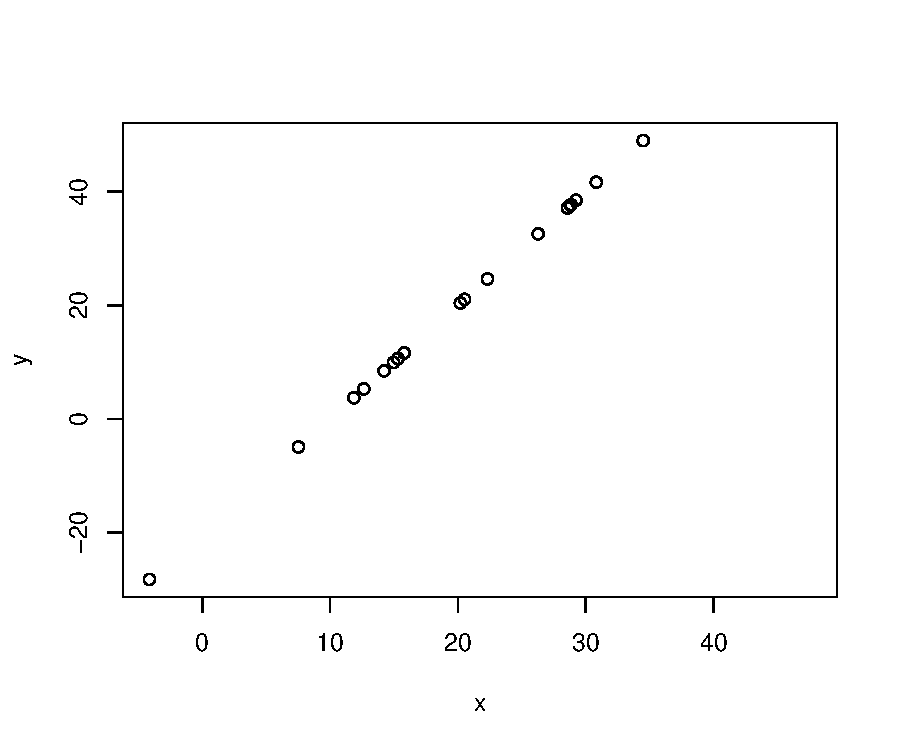
\includegraphics[width=\maxwidth]{figure/unnamed-chunk-89-1} 

\end{knitrout}
\caption{ Scatterplot}\label{fig:scatterplot}
\end{center}
\end{figure}

\begin{answerlist}
  \item The standard deviation of $Y$ is at least $6$.
  \item For $X =  13.6 $, $Y$ can be expected to be about  -44 .
  \item La pendenza della retta di regressione ? circa $1$.
  \item The mean of $X$ is at most $5$.
  \item The absolute value of the correlation coefficient is at most $0.8$.
\end{answerlist}
\end{question}

%% SOLUTIONS
\begin{solution}
\begin{answerlist}
  \item \\textbf{True}: The standard deviation of $Y$ is about equal to $ 20 $ and is therefore larger than $6$.
  \item \\textbf{False}: The regression line at $X=13.6$ implies a value of about $Y = 7.2$.
  \item \\textbf{False}: The slope of the regression line is given by $r \\cdot s_y/s_x$ and hence not about equal to $1$.
  \item \\textbf{False}: The mean of $X$ is about equal to $ 20 $ and hence is larger than $5$.
  \item \\textbf{False}: A strong association between the variables is given in the scatterplot. Hence the absolute value of the correlation coefficient is close to $1$ and therefore larger than $0.8$.
\end{answerlist}
\end{solution}
\end{itemize}
%% META-INFORMATION
%% \extype{mchoice}
%% \exsolution{mchoice2string(solutions)}
%% \exname{Multiple choice}

\end{comment}

 \subsection{Distribuzione normale}


Spesso  i dati sperimentali presentano una distribuzione a  campana del tipo che segue

\begin{knitrout}
\definecolor{shadecolor}{rgb}{0.969, 0.969, 0.969}\color{fgcolor}
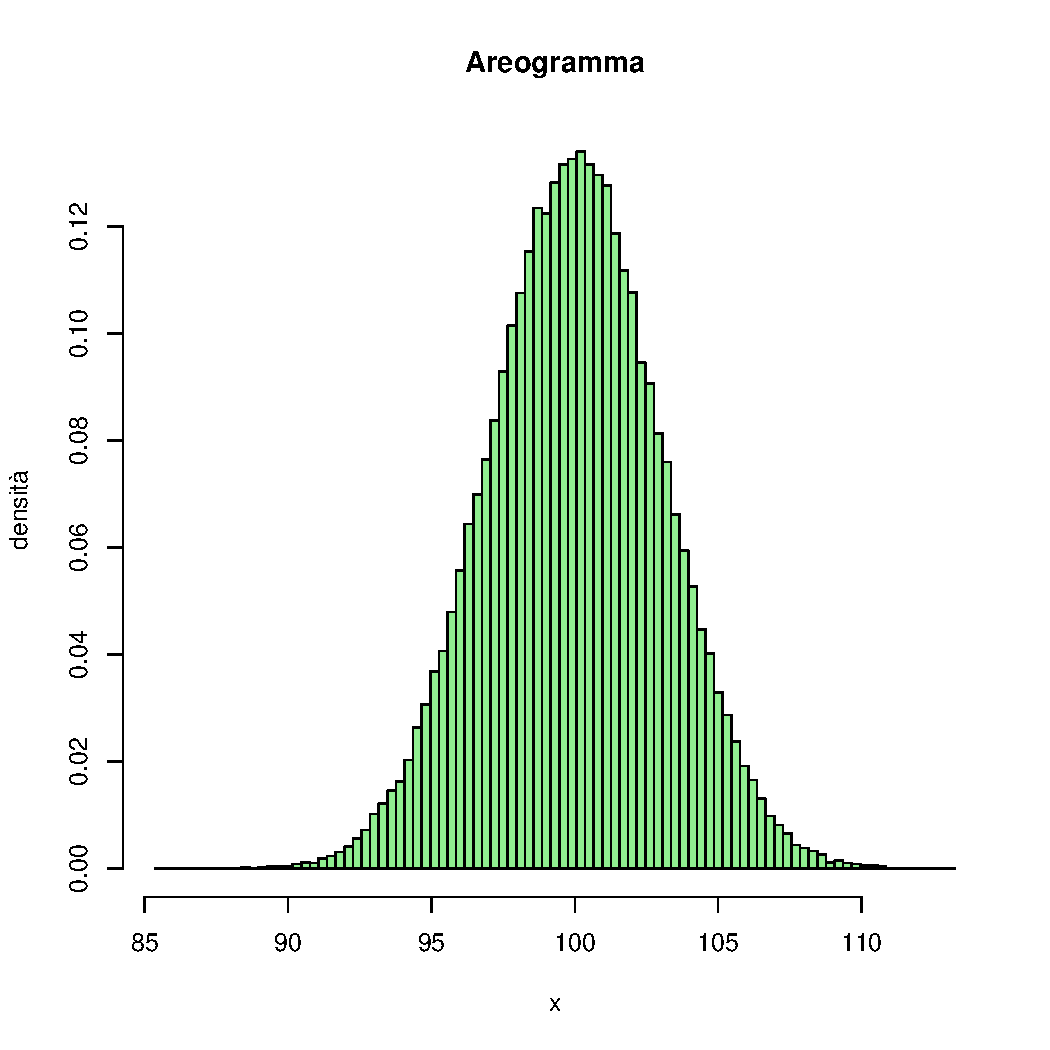
\includegraphics[width=\maxwidth]{figure/unnamed-chunk-91-1} 

\end{knitrout}

Sovrapponiamo ora all'areogramma una curva che sembra approssimare molto bene l'areogramma. 


\begin{knitrout}
\definecolor{shadecolor}{rgb}{0.969, 0.969, 0.969}\color{fgcolor}
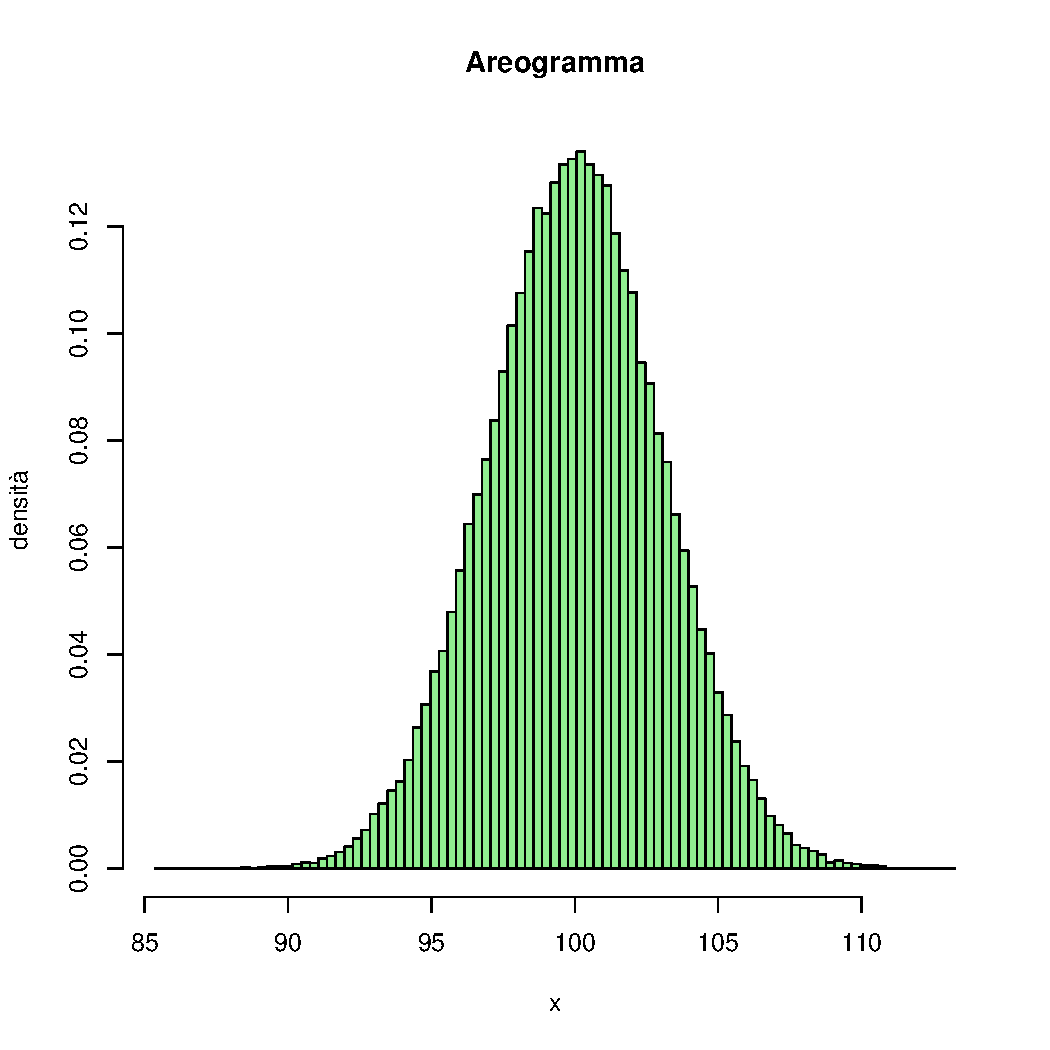
\includegraphics[width=\maxwidth]{figure/unnamed-chunk-92-1} 

\end{knitrout}

La curva sovraimpressa al grafico si chiama **gaussiana** o curva a campana o *funzione di densità normale*. Tale curva è una densità di probabilità e descrive un tipo particolare di variabili aleatorie continue.

L'espressione analitica  dipende da due parametri $\mu$ e $\sigma$,  che coincidono con la media e la deviazione standard della variabile corrispondente:


$$\textrm{dnorm}(x,\mu,\sigma)=\frac{1}{\sigma\sqrt{2 \pi} } \textrm{e}^{-\frac{(x - \mu)^2}{2 \sigma^2}}$$

Abbiamo scritto qui direttamente l'espressione $\textrm{dnorm}(x,\mu,\sigma)$ senza preoccuparci di verificare che

Verifica 1:  l'integrale è 1 [ossia la funzione è una densità di probabilità]

Verifica 2: il valore atteso è $\mu$
 
Verifica 3: la varianza è $\sigma^2$

La conoscenza di $\mu$ e $\sigma$ caratterizza completamente una variabile gaussiana.  La probabilità che una variabile gaussiana assuma il valore nell'intervallo $[a,b]$ è uguale all'area sottesa alla corrispondente curva normale nell'intervallo $[a,b]$.


Riportiamo in figura  il grafico di alcune gaussiane riportando i valori dei parametri  $\mu$ e $\sigma$

\begin{knitrout}
\definecolor{shadecolor}{rgb}{0.969, 0.969, 0.969}\color{fgcolor}
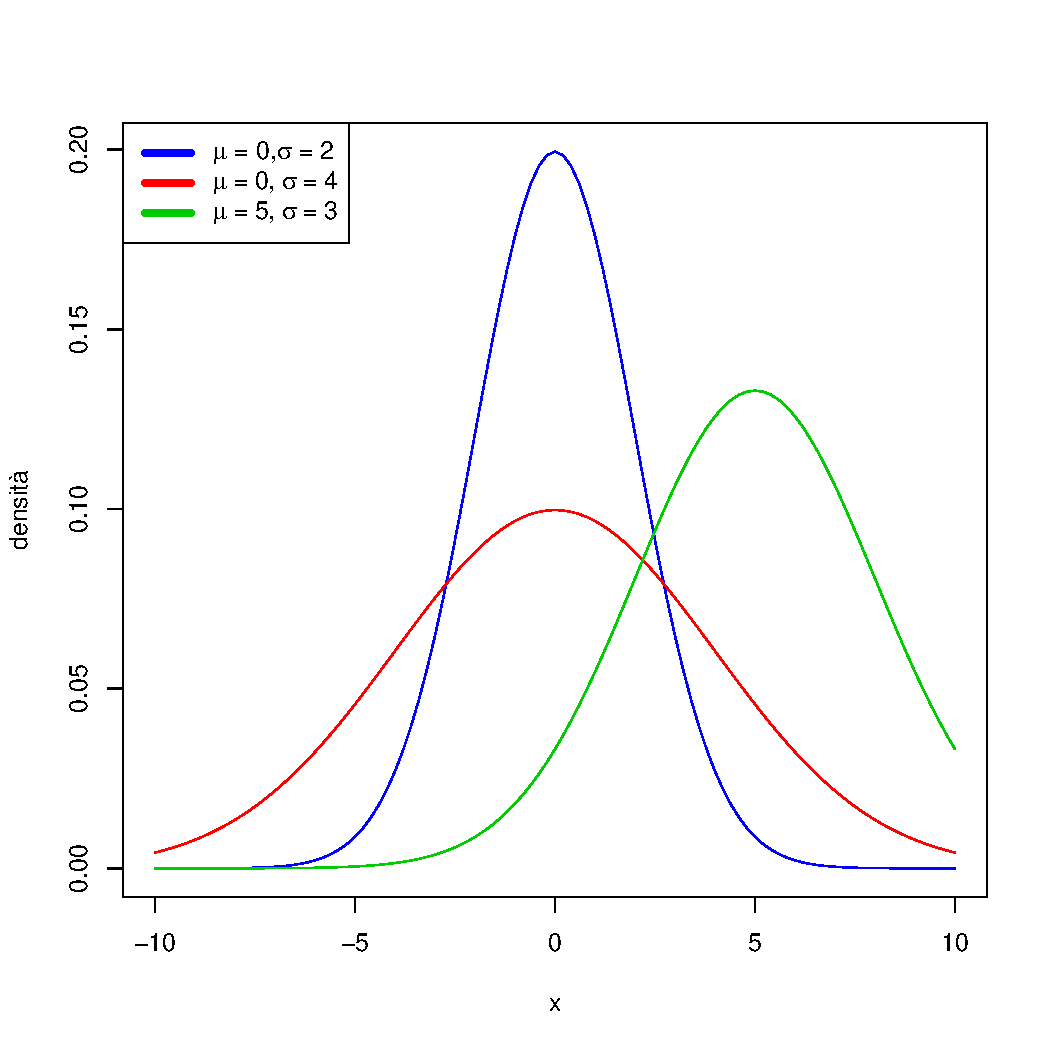
\includegraphics[width=\maxwidth]{figure/unnamed-chunk-93-1} 

\end{knitrout}

\subsubsection{La funzione \texttt{dnorm}}

Come appena visto \textsf{R }indica con il nome \texttt{dnorm}, la densit\`a normale o gaussiana. Essa accetta come parametri sia la media $\mu$ che la deviazione standard $\sigma$ come \`e possibile verificare con il comando \texttt{formals} che ci fornisce gli argomenti di una funzione e gli eventuali valori preassegnati.
\begin{knitrout}
\definecolor{shadecolor}{rgb}{0.969, 0.969, 0.969}\color{fgcolor}\begin{kframe}
\begin{alltt}
\hlkwd{formals}\hlstd{(dnorm)}
\end{alltt}
\begin{verbatim}
## $x
## 
## 
## $mean
## [1] 0
## 
## $sd
## [1] 1
## 
## $log
## [1] FALSE
\end{verbatim}
\end{kframe}
\end{knitrout}
Se i parametri sono omessi \texttt{dnorm} rappresenta la densit\`a normale standard con $\mu=0$ e $\sigma=1$.
Il grafico~(\ref{fig:normalesta}) della gaussiana
 tra due estremi, ad esempio -2.5 e 2.5 si ottiene con il solito comando
\begin{knitrout}
\definecolor{shadecolor}{rgb}{0.969, 0.969, 0.969}\color{fgcolor}\begin{kframe}
\begin{alltt}
\hlkwd{curve}\hlstd{(dnorm,}\hlopt{-}\hlnum{2.5}\hlstd{,}\hlnum{2.5}\hlstd{)}
\end{alltt}
\end{kframe}
\end{knitrout}

\begin{figure}[htbp]
\begin{center}
\begin{knitrout}
\definecolor{shadecolor}{rgb}{0.969, 0.969, 0.969}\color{fgcolor}
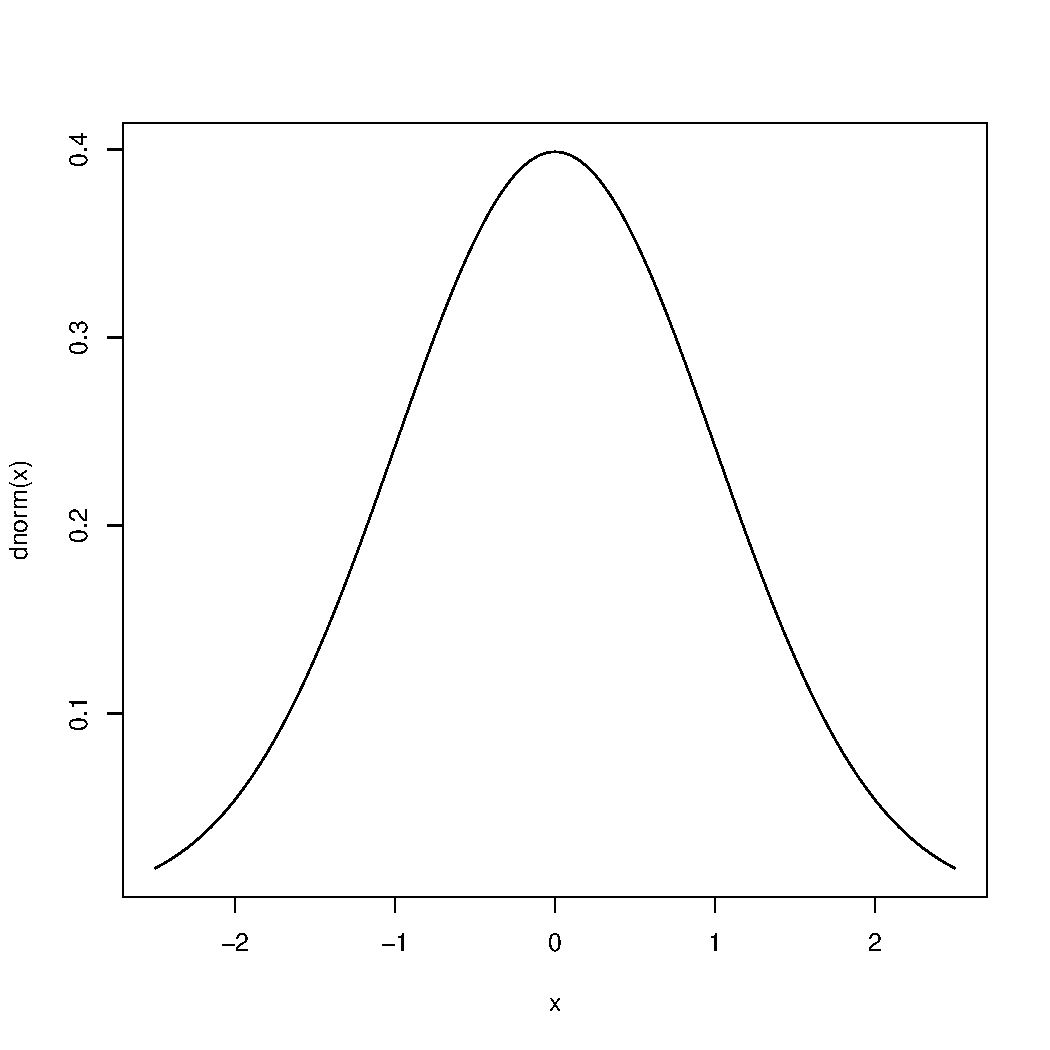
\includegraphics[width=\maxwidth]{figure/unnamed-chunk-96-1} 

\end{knitrout}
\caption{ Grafico della normale standard nell'intervallo $[-2.5,2.5]$. }
\label{fig:normalesta}
\end{center}
\end{figure}
Per  visualizzare una gaussiana non standard, ad esempio una gaussiana con media $\mu=1$ e  deviazione standard $\sigma=1.5$, tra -3 e 3. scriveremo invece
\begin{knitrout}
\definecolor{shadecolor}{rgb}{0.969, 0.969, 0.969}\color{fgcolor}\begin{kframe}
\begin{alltt}
\hlkwd{curve}\hlstd{(}\hlkwd{dnorm}\hlstd{(x,}\hlkwc{mean}\hlstd{=}\hlnum{1}\hlstd{,}\hlkwc{sd}\hlstd{=}\hlnum{1.5}\hlstd{),}\hlopt{-}\hlnum{3}\hlstd{,}\hlnum{3}\hlstd{)}
\end{alltt}
\end{kframe}
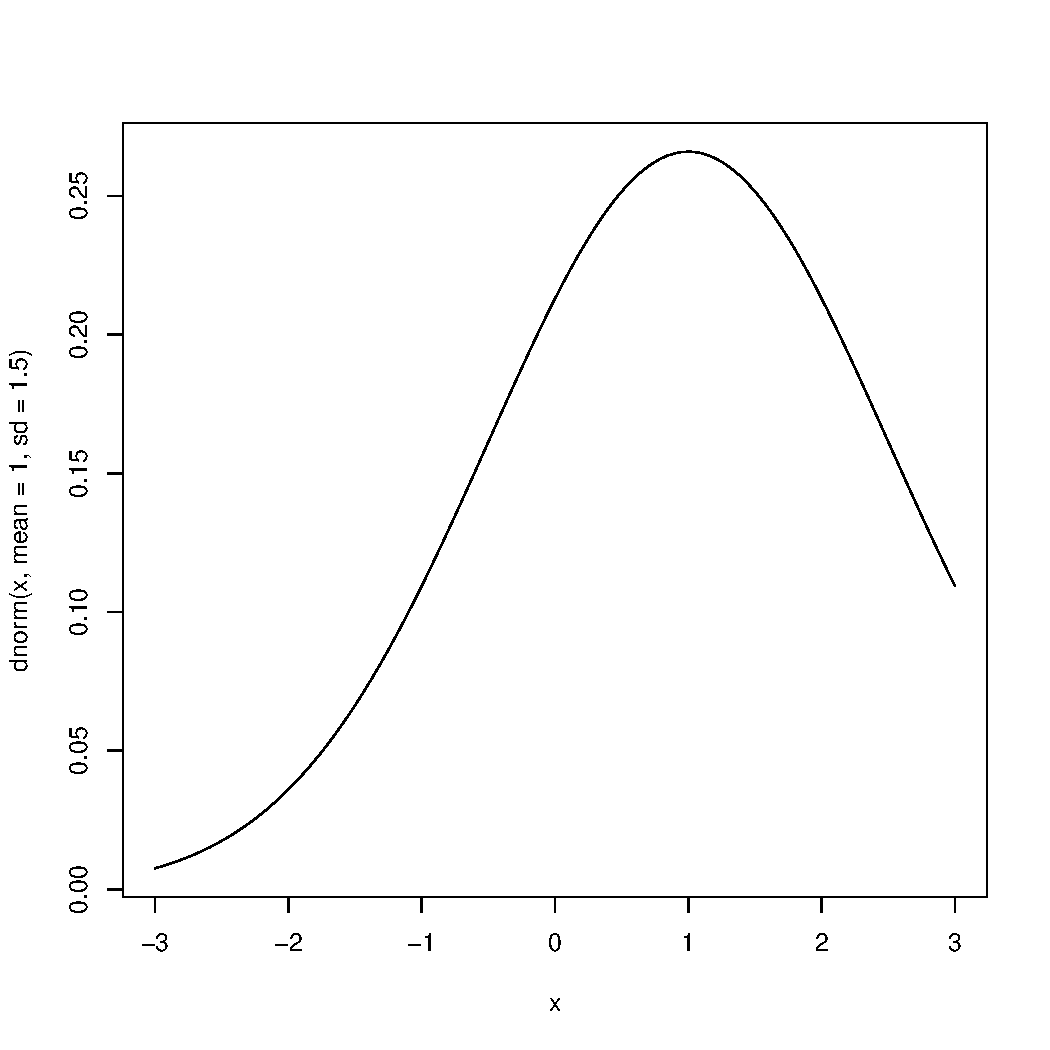
\includegraphics[width=\maxwidth]{figure/unnamed-chunk-97-1} 

\end{knitrout}
\subsection{La funzione \texttt{pnorm}}
La funzione \texttt{pnorm}(\varia{x})   \`e la antiderivata di \texttt{dnorm} calcolata come segue
\begin{equation*}\texttt{pnorm}(\varia{x}) =\int_{-\infty}^x  \texttt{dnorm}(s)ds
\end{equation*}
Ovviamente
$$\int_a^b \texttt{dnorm}(x)dx=\texttt{pnorm}(b)-\texttt{pnorm}(a)$$
e per avere l'area sottesa tra $3$ e $5$  basta scrivere:
\begin{knitrout}
\definecolor{shadecolor}{rgb}{0.969, 0.969, 0.969}\color{fgcolor}\begin{kframe}
\begin{alltt}
\hlkwd{pnorm}\hlstd{(}\hlnum{5}\hlstd{)}\hlopt{-}\hlkwd{pnorm}\hlstd{(}\hlnum{3}\hlstd{)}
\end{alltt}
\begin{verbatim}
## [1] 0.001349611
\end{verbatim}
\end{kframe}
\end{knitrout}

Per ottenere il valore dell'area tra 0 e $x$ bisogna allora sottrarre \texttt{pnorm}(0)=0.5 all'area fornita dalla funzione.
Per cui possiamo scrivere:
\begin{knitrout}
\definecolor{shadecolor}{rgb}{0.969, 0.969, 0.969}\color{fgcolor}\begin{kframe}
\begin{alltt}
\hlkwd{pnorm}\hlstd{(}\hlnum{1}\hlstd{)}\hlopt{-}\hlnum{0.5}
\end{alltt}
\begin{verbatim}
## [1] 0.3413447
\end{verbatim}
\end{kframe}
\end{knitrout}


\subsection{La funzione \texttt{qnorm} e la tabella della densit\`a di Gauss}


La funzione \texttt{qnorm} rappresenta la funzione inversa di \texttt{pnorm}.
\[\texttt{qnorm}(A)=x\Leftrightarrow A=\int_{-\infty}^x \texttt{dnorm}(s)ds\] 
come illustrato nella figura~\ref{fig:fig2code}.
\begin{center}
\begin{figure}[H]
\begin{knitrout}
\definecolor{shadecolor}{rgb}{0.969, 0.969, 0.969}\color{fgcolor}
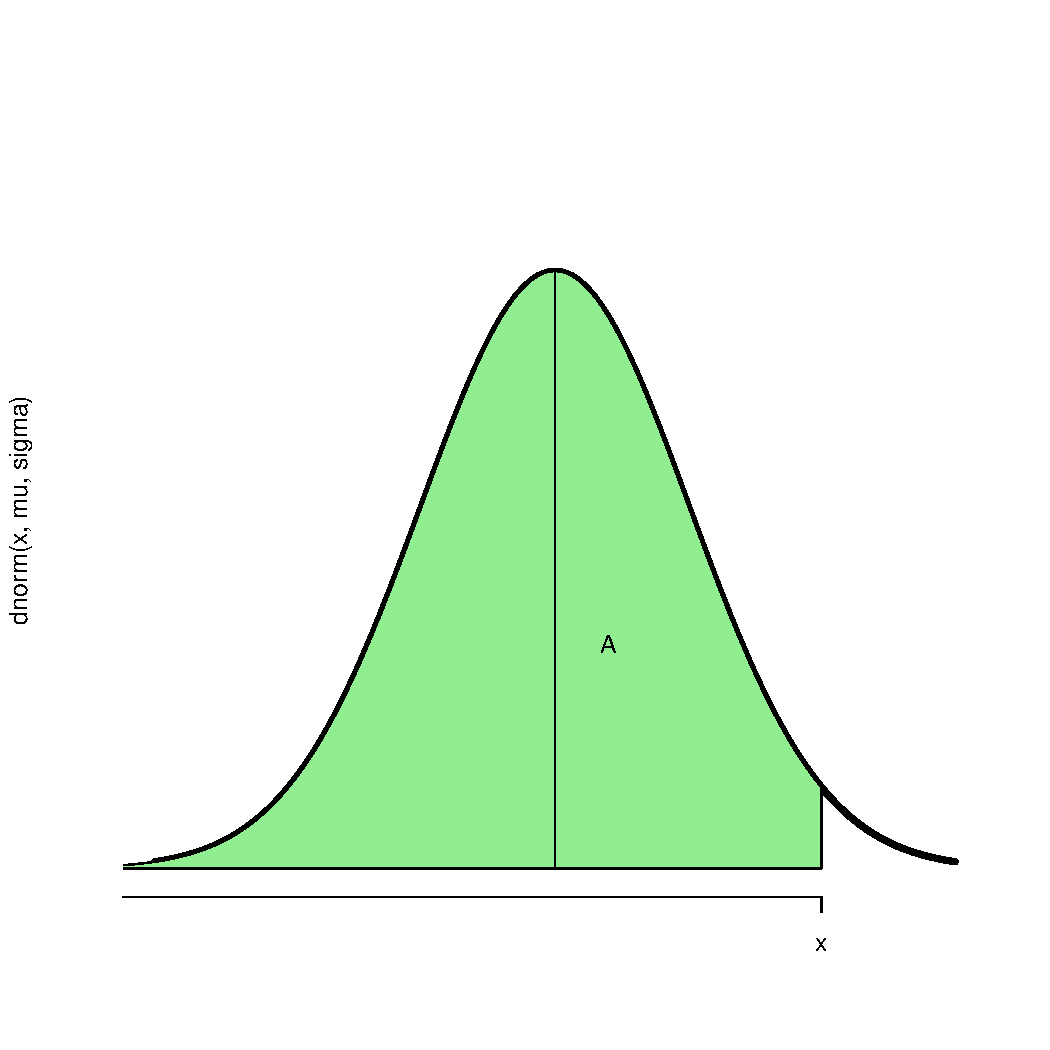
\includegraphics[width=\maxwidth]{figure/unnamed-chunk-101-1} 

\end{knitrout}
\caption{$x=\texttt{qnorm}(A)$}
\label{fig:fig2code}
\end{figure}
\end{center}
Vogliamo costruire una funzione, diciamo $U$ tale che assegnato un valore di area $A$   fornisca l'ascissa $x=U(A)$ come in figura~\ref{fig:fig12code} in modo che l'area tra - $x$ e $x$ sia esattamente pari ad $A$.  

\begin{figure}[H]
\begin{knitrout}
\definecolor{shadecolor}{rgb}{0.969, 0.969, 0.969}\color{fgcolor}
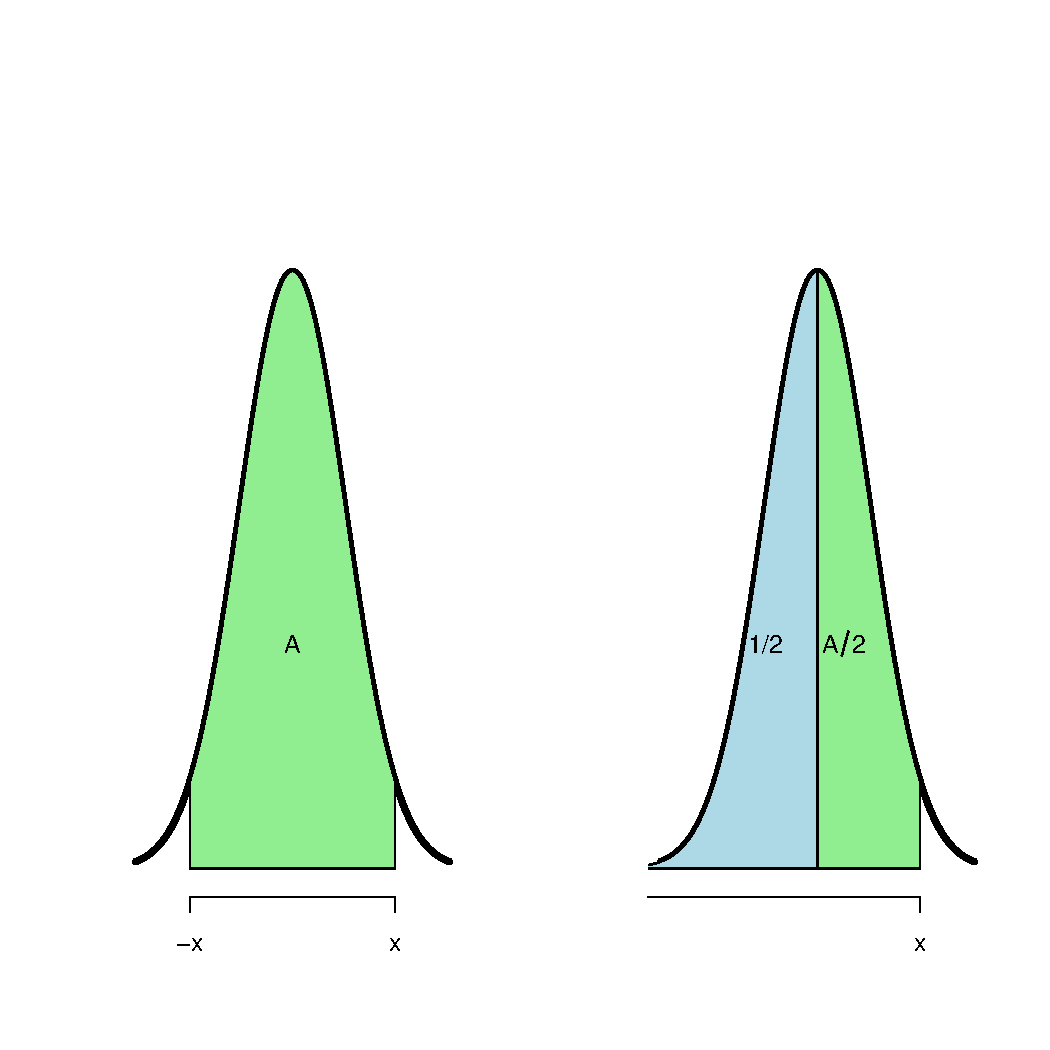
\includegraphics[width=\maxwidth]{figure/unnamed-chunk-102-1} 

\end{knitrout}
\caption{$x=U(A)=\texttt{qnorm}(1/2+A/2)$}
\label{fig:fig12code}
\end{figure}
Dalla stessa figura  si evince che la funzione che riproduce la tabella è
\begin{knitrout}
\definecolor{shadecolor}{rgb}{0.969, 0.969, 0.969}\color{fgcolor}\begin{kframe}
\begin{alltt}
\hlstd{U} \hlkwb{<-}\hlkwa{function} \hlstd{(}\hlkwc{A}\hlstd{)} \hlkwd{qnorm} \hlstd{(}\hlnum{1}\hlopt{/}\hlnum{2} \hlopt{+} \hlstd{A}\hlopt{/}\hlnum{2}\hlstd{)}
\end{alltt}
\end{kframe}
\end{knitrout}
Questa funzione fornisce fissato il livello di fiducia l'ascissa $x$  tale che l'intervallo simmetrico $[-x,x]$ racchiuda un'area pari al lvello di fiducia. Per esempio
\begin{knitrout}
\definecolor{shadecolor}{rgb}{0.969, 0.969, 0.969}\color{fgcolor}\begin{kframe}
\begin{alltt}
\hlkwd{U}\hlstd{(}\hlnum{0.95}\hlstd{)}
\end{alltt}
\begin{verbatim}
## [1] 1.959964
\end{verbatim}
\end{kframe}
\end{knitrout}
\begin{figure}[H]
\begin{center}

\begin{knitrout}
\definecolor{shadecolor}{rgb}{0.969, 0.969, 0.969}\color{fgcolor}
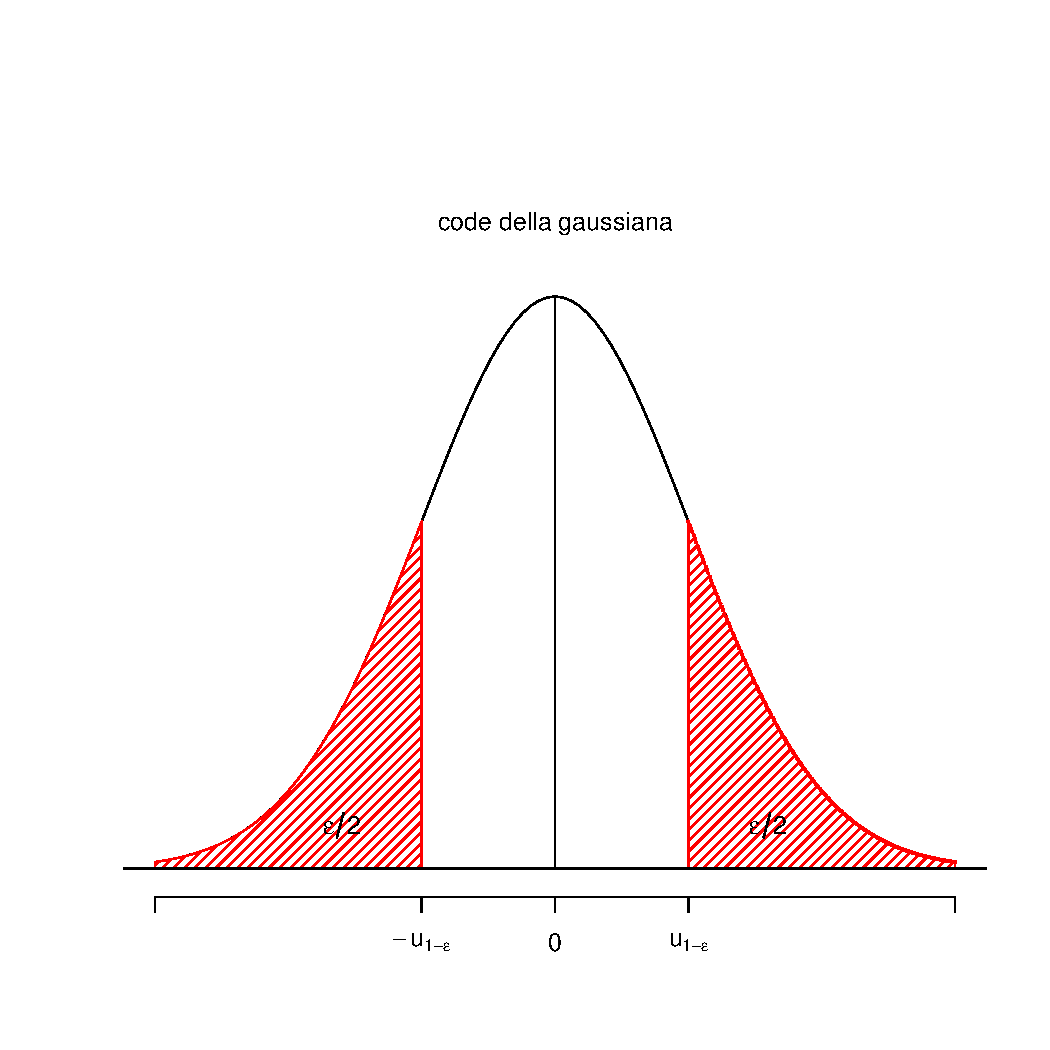
\includegraphics[width=\maxwidth]{figure/unnamed-chunk-106-1} 

\end{knitrout}
\caption{Code della distribuzione normale}
\label{fig:normaletratto}
\end{center}
\end{figure}

 \subsection{La funzione \texttt{rnorm}}
\`E possibile generare dei valori standardizzati casuali (media uguale a 0, deviazione standard pari a 1) che seguono la distribuzione normale standard. Basta semplicemente definire il numero di valori desiderati.
Il comando nella sua espressione generale \`e:
\begin{equation}\texttt{rnorm}(n,\texttt{mean}=\varia{valore}_1,\texttt{sd}=\varia{valore}_2)\end{equation}
Nel caso in cui volessimo una lista di 20 valori di una variabile normale con media assegnata 5 e deviazione standard 1 scriveremo
\begin{knitrout}
\definecolor{shadecolor}{rgb}{0.969, 0.969, 0.969}\color{fgcolor}\begin{kframe}
\begin{alltt}
\hlkwd{rnorm}\hlstd{(}\hlnum{20}\hlstd{,}\hlkwc{mean}\hlstd{=}\hlnum{5}\hlstd{,}\hlkwc{sd}\hlstd{=}\hlnum{1}\hlstd{)}
\end{alltt}
\begin{verbatim}
##  [1] 5.589574 5.004720 4.893384 4.592434 4.149222
##  [6] 5.800701 3.413862 5.977933 5.647532 5.716087
## [11] 4.879172 3.508112 5.603088 6.769773 6.335866
## [16] 4.410993 4.866959 3.490076 5.185364 3.976624
\end{verbatim}
\end{kframe}
\end{knitrout}
\subsection{La distribuzione $t$ di Student}
In \textsf{R} la distribuzione di Student \`e indicata con la lettera  \texttt{t}.  Come per le altre distribuzioni  si possono considerare le funzioni\vskip5pt
\begin{tabular}{|r|r |}
\hline
dt  &densit\`a\\
pt  &primitiva\\
qt & quantili\\
rt  &generatore random\\
\hline
\end{tabular}
\vskip10pt
Il grafico della distribuzione di Student ad un certo numero \texttt{df} di gradi di libert\`a  si ottiene con il comando
\begin{equation*}
\texttt{curve(dt(x},\texttt{df}),\varia{a},\varia{b})
\end{equation*}
Tracciamo ad esempio un grafico tra -2 e 2 per una distribuzione a 10 gradi di libert\`a (vedi figura ~(\ref{fig:graficostudent1})):

\begin{figure}[H]
\begin{center}
\begin{knitrout}
\definecolor{shadecolor}{rgb}{0.969, 0.969, 0.969}\color{fgcolor}\begin{kframe}
\begin{alltt}
\hlkwd{curve}\hlstd{(}\hlkwd{dt}\hlstd{(x,}\hlnum{10}\hlstd{),}\hlopt{-}\hlnum{2}\hlstd{,}\hlnum{2}\hlstd{)}
\end{alltt}
\end{kframe}
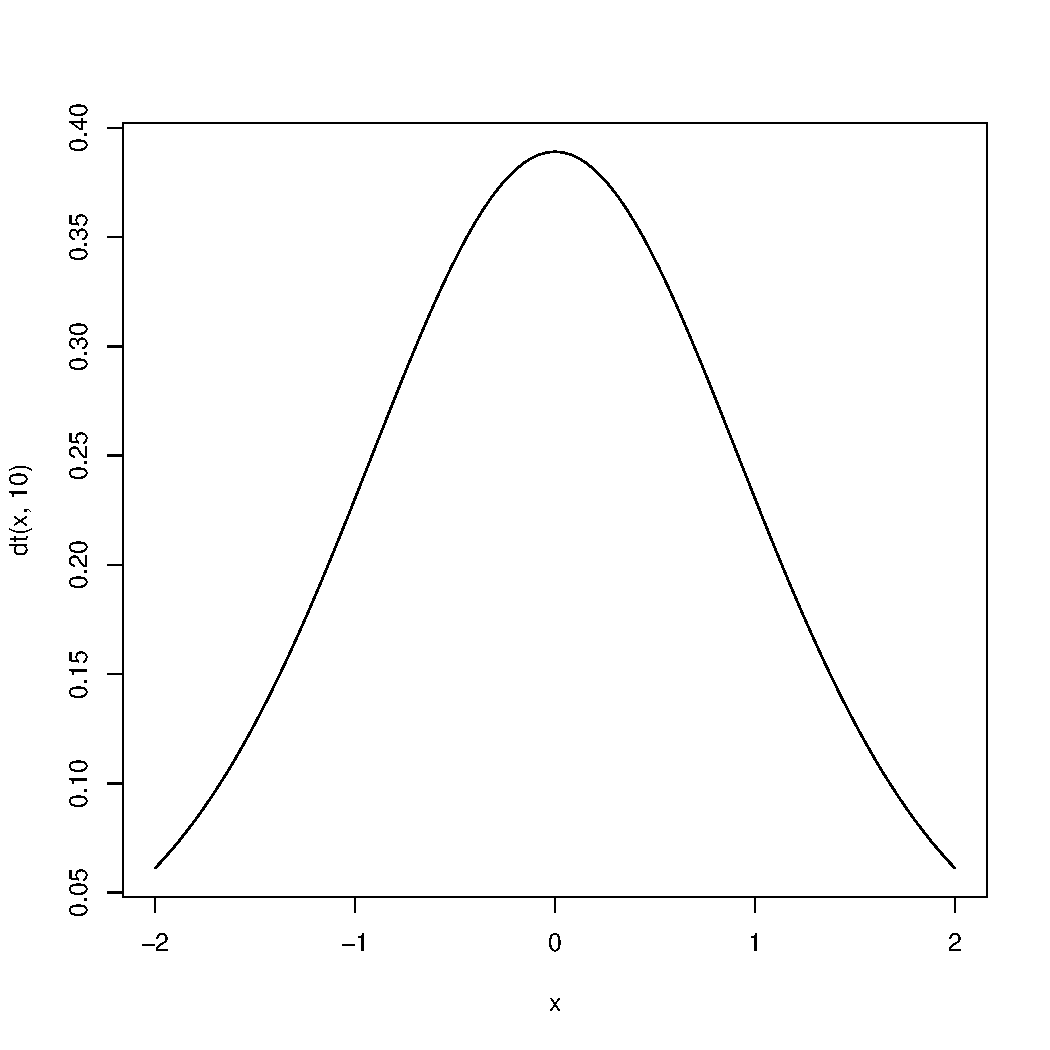
\includegraphics[width=\maxwidth]{figure/unnamed-chunk-108-1} 

\end{knitrout}
\caption{Grafico della distribuzione di Student a 10 gradi di libert\`a. }
\label{fig:graficostudent1}
\end{center}
\end{figure}
Ricordiamo che la distribuzione di Student si usa in  particolare nei casi in cui la deviazione standard della popolazione $\sigma$  non \`e conosciuta e viene rimpiazzata  dalla deviazione standard campionaria  $S$, calcolata con un numero $N$ di dati e quindi con $N-1$ gradi di libert\`a. Quando per\`o il numero di dati si avvicina a 30 la curva di Student \`e praticamente sovrapposta a quella della distribuzione normale, come mostra il grafico~(\ref{fig:graficostudent}):

\begin{figure}[H]
\begin{center}
\begin{knitrout}
\definecolor{shadecolor}{rgb}{0.969, 0.969, 0.969}\color{fgcolor}\begin{kframe}
\begin{alltt}
\hlkwd{curve}\hlstd{(}\hlkwd{dnorm}\hlstd{(x),}\hlopt{-}\hlnum{2}\hlstd{,}\hlnum{2}\hlstd{,}\hlkwc{col}\hlstd{=}\hlnum{3}\hlstd{)}
\hlkwd{curve}\hlstd{(}\hlkwd{dt}\hlstd{(x,}\hlnum{2}\hlstd{),}\hlopt{-}\hlnum{2}\hlstd{,}\hlnum{2}\hlstd{,}\hlkwc{col}\hlstd{=}\hlnum{1}\hlstd{,}\hlkwc{add}\hlstd{=T)}
\hlkwd{curve}\hlstd{(}\hlkwd{dt}\hlstd{(x,}\hlnum{25}\hlstd{),}\hlopt{-}\hlnum{2}\hlstd{,}\hlnum{2}\hlstd{,}\hlkwc{col}\hlstd{=}\hlnum{2}\hlstd{,}\hlkwc{add}\hlstd{=T)}
\hlkwd{legend}\hlstd{(}\hlstr{"topleft"}\hlstd{,} \hlkwd{c}\hlstd{(}\hlstr{"df=2"}\hlstd{,}\hlstr{"df=25"}\hlstd{,}\hlstr{"normale"}\hlstd{),}\hlkwc{pch}\hlstd{=}\hlnum{15}\hlstd{,}\hlkwc{col}\hlstd{=}\hlnum{1}\hlopt{:}\hlnum{3}\hlstd{);}
\end{alltt}
\end{kframe}
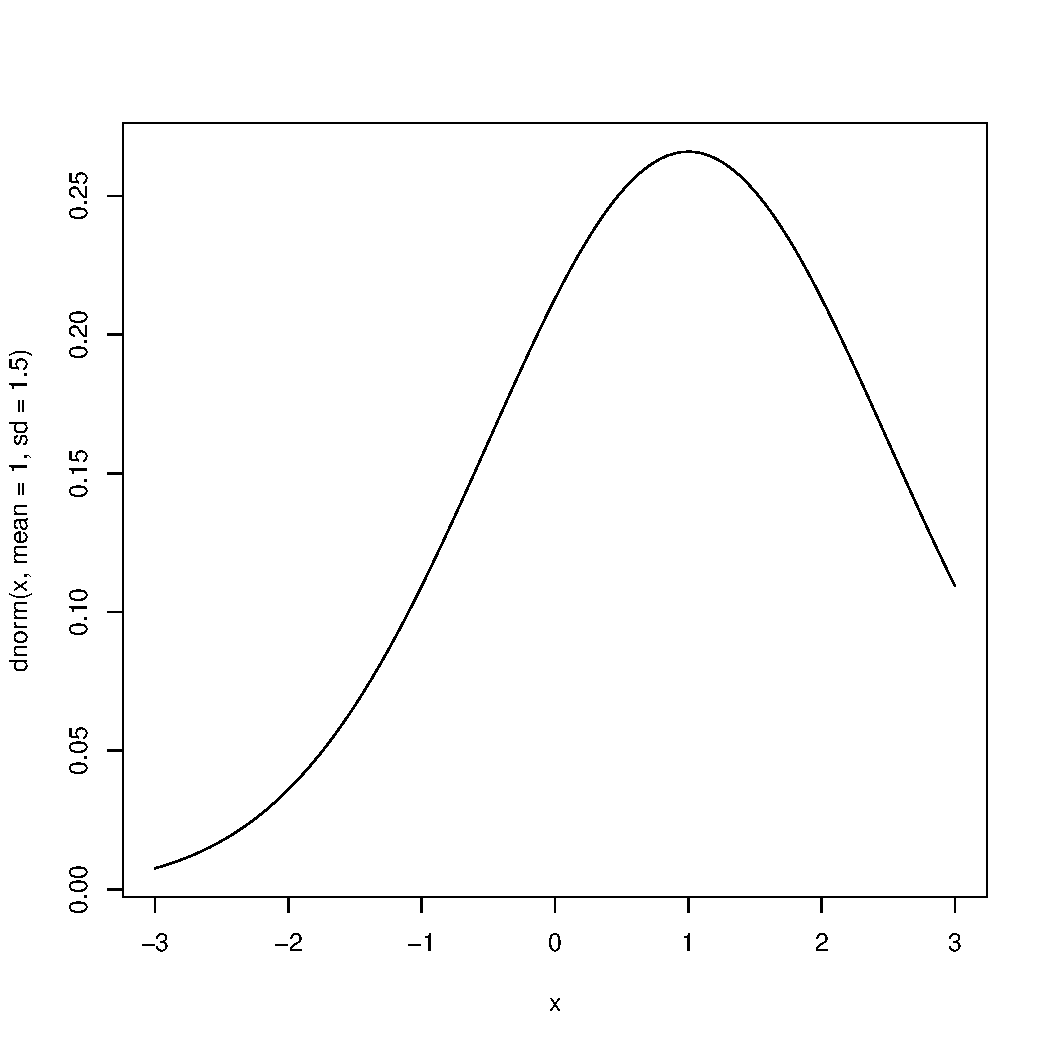
\includegraphics[width=\maxwidth]{figure/unnamed-chunk-109-1} 

\end{knitrout}
\caption{Grafico della distribuzione di Student a 10 gradi di libert\`a. }
\label{fig:graficostudent}
\end{center}
\end{figure}
Come nel caso della distribuzione normale se vogliamo una funzione diciamo \texttt{student}  tale che assegnato un valore di area $A$   fornisca l'ascissa $x=student(A)$  in modo che l'area tra - $x$ e $x$ sia esattamente pari ad $A$ dobbiamo scrivere la funzione
\begin{knitrout}
\definecolor{shadecolor}{rgb}{0.969, 0.969, 0.969}\color{fgcolor}\begin{kframe}
\begin{alltt}
\hlstd{student}\hlkwb{<-}\hlkwa{function} \hlstd{(}\hlkwc{A}\hlstd{,}\hlkwc{..}\hlstd{)} \hlkwd{qt} \hlstd{(}\hlnum{1}\hlopt{/}\hlnum{2} \hlopt{+} \hlstd{A}\hlopt{/}\hlnum{2}\hlstd{,..)}
\end{alltt}
\end{kframe}
\end{knitrout}
dove i puntini stanno per le variabili omesse o pi\`u esplicitamente
\begin{knitrout}
\definecolor{shadecolor}{rgb}{0.969, 0.969, 0.969}\color{fgcolor}\begin{kframe}
\begin{alltt}
\hlstd{student}\hlkwb{<-}\hlkwa{function} \hlstd{(}\hlkwc{A}\hlstd{,}\hlkwc{df}\hlstd{)} \hlkwd{qt} \hlstd{(}\hlnum{1}\hlopt{/}\hlnum{2} \hlopt{+} \hlstd{A}\hlopt{/}\hlnum{2}\hlstd{,df)}
\end{alltt}
\end{kframe}
\end{knitrout}
dove \texttt{df} sono i gradi di libert\`a. 
\subsection
{Regione di accettazione, intervalli di confidenza e test di Student}

Consideriamo ora una variabile normale $X$. Se ipotizziamo che il valore atteso di $X$ sia   $\mu$ (ipotesi nulla) allora il consuntivo 
\[T=\dfrac{M_N(X)-\mu}{S_X}\sqrt {N}\]
\`e distribuito secondo la distribuzione di Student a $N-1$ gradi di libert\`a. 
Se consideriamo una variabile distribuita secondo la distribuzione di Student, esattamente come nel caso della normale, possiamo determinare un valore $x$ dipendente dal livello di fiducia \texttt{f} e dai gradi di libert\`a 
$x=x(\texttt {f},df)$ tale che nell'intervallo $[-x,x]$ si concentri una probabilit\`a pari a \texttt{f}.

Applicando quanto detto a $T$ possiamo scrivere
\[ P(-x(\texttt {f},df)<T<x(\texttt {f},df))=\ \texttt {f}\]

Questo fatto consente di procedere in due direzioni.
\begin{itemize}
\item Test di ipotesi sul valore di $\mu$.
\item Intervallo di confidenza per $\mu$. 
\end{itemize}
 
Mostriamo come si può procedere:  
 
La funzione di
\textsf{R} che esegue il test di Student nelle sue diverse forme \`e  \texttt{t.test}.   Nella sua forma pi\`u semplice

\begin{knitrout}
\definecolor{shadecolor}{rgb}{0.969, 0.969, 0.969}\color{fgcolor}\begin{kframe}
\begin{alltt}
\hlstd{x}\hlkwb{=}\hlnum{1}\hlopt{:}\hlnum{20}\hlstd{;}  \hlkwd{t.test}\hlstd{(x)}
\end{alltt}
\begin{verbatim}
## 
## 	One Sample t-test
## 
## data:  x
## t = 7.9373, df = 19, p-value = 0.0000001884
## alternative hypothesis: true mean is not equal to 0
## 95 percent confidence interval:
##   7.731189 13.268811
## sample estimates:
## mean of x 
##      10.5
\end{verbatim}
\end{kframe}
\end{knitrout}
Possiamo anche eseguire specificare l'ipotesi sul valore di $\mu$:
\begin{knitrout}
\definecolor{shadecolor}{rgb}{0.969, 0.969, 0.969}\color{fgcolor}\begin{kframe}
\begin{alltt}
\hlkwd{t.test}\hlstd{(x,}\hlkwc{mu}\hlstd{=}\hlnum{7}\hlstd{)}
\end{alltt}
\begin{verbatim}
## 
## 	One Sample t-test
## 
## data:  x
## t = 2.6458, df = 19, p-value = 0.01595
## alternative hypothesis: true mean is not equal to 7
## 95 percent confidence interval:
##   7.731189 13.268811
## sample estimates:
## mean of x 
##      10.5
\end{verbatim}
\end{kframe}
\end{knitrout}
Possiamo infine specificare l'ipotesi alternativa. Per esempio se l'ipotesi alternativa \`e
\texttt{\virgolette less\virgolette}  il risultato del test cambia completamente.
\begin{knitrout}
\definecolor{shadecolor}{rgb}{0.969, 0.969, 0.969}\color{fgcolor}\begin{kframe}
\begin{alltt}
\hlkwd{t.test}\hlstd{(x,}\hlkwc{mu}\hlstd{=}\hlnum{7}\hlstd{,} \hlkwc{alternative}\hlstd{=}\hlstr{"less"}\hlstd{)}
\end{alltt}
\begin{verbatim}
## 
## 	One Sample t-test
## 
## data:  x
## t = 2.6458, df = 19, p-value = 0.992
## alternative hypothesis: true mean is less than 7
## 95 percent confidence interval:
##      -Inf 12.78743
## sample estimates:
## mean of x 
##      10.5
\end{verbatim}
\end{kframe}
\end{knitrout}

In pratica ci viene fornito come $p$-value il valore dell'area sottesa dalla distribuzione di Student da $-\infty$ al valore di $t$ se l'ipotesi alternativa \`e  \texttt{\virgolette less\virgolette} e il valore dell'area sottesa dalla distribuzione di Student dal valore di $t$ a $+\infty$ se l'ipotesi alternativa \`e     \texttt{\virgolette greater\virgolette}  \subsection{Test di Student per dati appaiati}
Il test di Student per dati appaiati non \`e altro che un test di Student sulla differenza di 2 liste di dati di ugual lunghezza. Consideriamo ad esempio il confronto di 2 tecniche di misura applicate agli stessi campioni
\begin{knitrout}
\definecolor{shadecolor}{rgb}{0.969, 0.969, 0.969}\color{fgcolor}\begin{kframe}
\begin{alltt}
\hlstd{x}\hlkwb{<-}\hlkwd{c}\hlstd{(}\hlnum{1.46}\hlstd{,}\hlnum{2.22}\hlstd{,}\hlnum{2.84}\hlstd{,}\hlnum{1.97}\hlstd{,}\hlnum{1.13}\hlstd{,}\hlnum{2.35}\hlstd{)}
\hlstd{y}\hlkwb{<-}\hlkwd{c}\hlstd{(}\hlnum{1.42}\hlstd{,}\hlnum{2.38}\hlstd{,}\hlnum{2.67}\hlstd{,}\hlnum{1.8}\hlstd{,}\hlnum{1.09}\hlstd{,}\hlnum{2.25}\hlstd{)}
\end{alltt}
\end{kframe}
\end{knitrout}

Possiamo calcolare la differenza \texttt{x-y} ed applicare il test di Student oppure ottenere lo stesso risultato specificando l'opzione \texttt{paired=TRUE}
\begin{knitrout}
\definecolor{shadecolor}{rgb}{0.969, 0.969, 0.969}\color{fgcolor}\begin{kframe}
\begin{alltt}
 \hlkwd{t.test}\hlstd{(x,y,}\hlkwc{paired}\hlstd{=}\hlnum{TRUE}\hlstd{)}
\end{alltt}
\begin{verbatim}
## 
## 	Paired t-test
## 
## data:  x and y
## t = 1.2, df = 5, p-value = 0.2839
## alternative hypothesis: true difference in means is not equal to 0
## 95 percent confidence interval:
##  -0.06852909  0.18852909
## sample estimates:
## mean of the differences 
##                    0.06
\end{verbatim}
\end{kframe}
\end{knitrout}

Il consuntivo   \texttt{t} cade entro la regione di accettazione del test.
\`E  possibile specificare il livello di fiducia da utilizzare per il test di Student come:

$$\texttt{conf.level}=\varia{numero}$$

Il comando completo di tutti i parametri  \`e quindi:
\begin{eqnarray*}
\texttt{t.test}(\varia{dati}_1,\varia{dati}_2,
\\
\texttt{paired=TRUE,conf.level}=\varia{valore})
\end{eqnarray*}
Ad esempio eseguiamo un $t$-test per dati appaiati, tra $x=(1,2,3,4)$ e $y=(3,2,4,5)$ con {\it confidence level} di 0.85. Scriveremo
\begin{knitrout}
\definecolor{shadecolor}{rgb}{0.969, 0.969, 0.969}\color{fgcolor}\begin{kframe}
\begin{alltt}
\hlkwd{t.test}\hlstd{(}\hlnum{1}\hlopt{:}\hlnum{4}\hlstd{,}\hlnum{5}\hlopt{:}\hlnum{2}\hlstd{,}\hlkwc{paired}\hlstd{=}\hlnum{TRUE}\hlstd{,}\hlkwc{conf.level}\hlstd{=}\hlnum{0.85}\hlstd{)}
\end{alltt}
\end{kframe}
\end{knitrout}
 Il consuntivo $t$ cade fuori dalla regione di accettazione proposta.


\subsection{t-test: caso ad egual varianza}

Si considerino i seguenti dati relativi alla misura di una grandezza fisica.


\[(
\color{red}{11.4},\color{blue}{23.7},\color{blue}{24.3},\color{red}{16.5},\color{blue}{28.5},
\color{blue}{26.6},\color{red}{21.1},\color{red}{29.9},\color{blue}{17.9},\color{red}{25.3},\color{blue}{14.2})\]


I colori rosso e blu si riferiscono all'utilizzo di due diversi strumenti di misura. Si noti che il numero di esperimenti in rosso (esperimenti 1,4, 7,8,10) non é uguale al numero di esperimenti in blu (esperimenti 2,3,5,6,9,11): non si tratta di misure ripetute sugli stessi campioni, ma di misure effettuate su campioni diversi.

Si dica, con fiducia al 95\% se esiste una differenza fra i due strumenti.
\begin{itemize}
\item I dati sono
\begin{knitrout}
\definecolor{shadecolor}{rgb}{0.969, 0.969, 0.969}\color{fgcolor}\begin{kframe}
\begin{verbatim}
## 11.4 16.5 21.1 29.9 25.3
## 23.7 24.3 28.5 26.6 17.9 14.2
\end{verbatim}
\end{kframe}
\end{knitrout}
\item Ipotesi di lavoro \[\mu_R= \mu_B\]
  \item Calcoliamo i valori dei parametri statistici per il campione rosso e per il campione blu.
\item Indicatori:
\[m_R=20.84\]
\[m_B=22.5333333\]
 \[s_R=7.2455504\]
\[s_B=5.4320039\]
\end{itemize}

Dobbiamo valutare il valore del consuntivo
\[ t_{ R, B} =\frac{ (M_R-M_B) -(\mu_R-\mu_B)}{\Sigma }\]
nell'ipotesi di lavoro 
\[\mu_R-\mu_B= 0\Leftrightarrow \mu_R=\mu_B\]

dove
\[
\begin{aligned}
\Sigma =& \sqrt{\dfrac{(n_R-1) S_R^2+(n_B-1) S_B^2 }{n_R+n_B-2}  \left(\frac{1}{n_R} +\frac{1}{n_B}\right)}\rightarrow  \\
&\sqrt{\dfrac{209.992+147.5333333 }{9}   \left(\frac{1}{5} +\frac{1}{6}\right)}= 
\sqrt{14.5658469} = 3.8165229
\end{aligned}
\] 

Il valore osservato di $t_{R,B}$ è

\[t_{ R,B} = \frac{m_R-m_B}{\Sigma}  =\ensuremath{-0.4436848} \]


La regione di accettazione \`e

\[[-t_{ 0.95, 9} , t_{0.95, 9} ] = [-2.262, 2.262]\]

Visto che il consuntivo  cade ampiamente in tale intervallo accettiamo l'ipotesi di lavoro.

con \rpr basta scrivere:
\begin{knitrout}
\definecolor{shadecolor}{rgb}{0.969, 0.969, 0.969}\color{fgcolor}\begin{kframe}
\begin{alltt}
\hlstd{R}\hlkwb{=}\hlkwd{c}\hlstd{(}\hlnum{11.4}\hlstd{,}\hlnum{16.5}\hlstd{,}\hlnum{21.1}\hlstd{,}\hlnum{29.9}\hlstd{,}\hlnum{25.3}\hlstd{)}
\hlstd{B}\hlkwb{=}\hlkwd{c}\hlstd{(}\hlnum{23.7}\hlstd{,}\hlnum{24.3}\hlstd{,}\hlnum{28.5}\hlstd{,}\hlnum{26.6}\hlstd{,} \hlnum{17.9}\hlstd{,}\hlnum{14.2}\hlstd{)}
\hlkwd{t.test}\hlstd{(R,B,}\hlkwc{var.equal}\hlstd{=T)}
\end{alltt}
\begin{verbatim}
## 
## 	Two Sample t-test
## 
## data:  R and B
## t = -0.44368, df = 9, p-value = 0.6677
## alternative hypothesis: true difference in means is not equal to 0
## 95 percent confidence interval:
##  -10.326908   6.940241
## sample estimates:
## mean of x mean of y 
##  20.84000  22.53333
\end{verbatim}
\end{kframe}
\end{knitrout}
Se non potessimo ipotizzare la provenienza dei due campioni da popolazioni con ugual varianza potremmo scrivere

\subsection{Caso generale (test di Welch)}

Qualora non si possa affermare l'eguaglianza delle varianze l'errore standard della differenza delle medie si può stimare come

\[ \Sigma= \sqrt{\frac{s_X^2}{n_X}+\frac{s_Y^2}{n_Y}}\]
\[ df =\dfrac
{ \left(\frac{s_X^2}{n_X}+\frac{s_Y^2}{n_Y}\right)^2}
{
\frac{(s_X^2/n_X)^2}{n_X-1}+
\frac{(s_Y^2/n_Y)^2}{n_Y-1}
}\]

Il consuntivo diviene

\[\frac{M_X-M_Y-(\mu_X-\mu_Y)}{\Sigma}  \]

e la regione di accettazione si calcola come

\[ [-t_{1-\epsilon,df},t_{1-\epsilon,df}]\]


\subsubsection{Esempio}
Con gli stessi dati di prima si ipotizzi $\mu_X=\mu_Y$ (fiducia al 95\%)

\[ X=(11.4, 16.5, 21.1, 29.9, 25.3)\quad Y=(23.7, 24.3, 28.5, 26.6, 17.9, 14.2)\]


\[ \Sigma= \sqrt{15.4173778}\]
e i gradi di libertà  
\[ df =\dfrac
{  (15.4173778)^2}
{
(110.2416002/4+
24.1845383/5)
}= \]
\[
  7.3368917
\]

Se si usa  \rpr basta scrivere

\begin{knitrout}
\definecolor{shadecolor}{rgb}{0.969, 0.969, 0.969}\color{fgcolor}\begin{kframe}
\begin{alltt}
\hlkwd{t.test}\hlstd{(X,Y)}
\end{alltt}
\begin{verbatim}
## 
## 	Welch Two Sample t-test
## 
## data:  X and Y
## t = -0.43126, df = 7.3369, p-value = 0.6787
## alternative hypothesis: true difference in means is not equal to 0
## 95 percent confidence interval:
##  -10.892293   7.505627
## sample estimates:
## mean of x mean of y 
##  20.84000  22.53333
\end{verbatim}
\end{kframe}
\end{knitrout}

\subsection{Test $\chi^2$  di indipendenza}

%code chunk
Consideriamo il seguente \emph{dataframe} che riporta le ambizioni di un gruppo di scolari americani
\begin{knitrout}
\definecolor{shadecolor}{rgb}{0.969, 0.969, 0.969}\color{fgcolor}\begin{kframe}
\begin{alltt}
\hlkwd{data}\hlstd{(bambini)}
\end{alltt}


{\ttfamily\noindent\color{warningcolor}{\#\# Warning in data(bambini): data set 'bambini' not found}}\begin{alltt}
\hlkwd{str}\hlstd{(bambini)}
\end{alltt}


{\ttfamily\noindent\bfseries\color{errorcolor}{\#\# Error in str(bambini): object 'bambini' not found}}\end{kframe}
\end{knitrout}

Nella tabella le colonne che ci interessano al momento sono quelle che riguardano il sesso, gli obiettivi (scelti tra successo scolastico, capacit\`a sportiva e popolarit\`a) e la provenienza (colonne 1, 5  e 7). Nelle colonne dalla 8 alla 11 sono messi in ordine di importanza per il conseguimento della popolarit\`a  voti, sport, aspetto esteriore e denaro.
%codechunk
 
Consideriamo per esempio le variabili provenienza e traguardi
\begin{knitrout}
\definecolor{shadecolor}{rgb}{0.969, 0.969, 0.969}\color{fgcolor}\begin{kframe}
\begin{alltt}
\hlstd{interessi2}\hlkwb{=}\hlstd{bambini[,}\hlkwd{c}\hlstd{(}\hlnum{5}\hlstd{,}\hlnum{7}\hlstd{)]}
\end{alltt}


{\ttfamily\noindent\bfseries\color{errorcolor}{\#\# Error in eval(expr, envir, enclos): object 'bambini' not found}}\begin{alltt}
\hlstd{tabella}\hlkwb{=}\hlkwd{table}\hlstd{(interessi2)}
\end{alltt}


{\ttfamily\noindent\bfseries\color{errorcolor}{\#\# Error in table(interessi2): object 'interessi2' not found}}\begin{alltt}
\hlstd{tabella}
\end{alltt}


{\ttfamily\noindent\bfseries\color{errorcolor}{\#\# Error in eval(expr, envir, enclos): object 'tabella' not found}}\end{kframe}
\end{knitrout}
 
Il test $\chi^2$  di indipendenza consente di  verificare se  due variabili sono indipendenti.
Se consideriamo le due variabili precedenti sesso e interessi.
\textsf{R}  dispone del comando \texttt{chisq.test},\index{\texttt{chisq.tst},test $\chi^2$}
dalla sintassi generale:$$\texttt{chisq.test}(\varia{tabella})$$
\begin{knitrout}
\definecolor{shadecolor}{rgb}{0.969, 0.969, 0.969}\color{fgcolor}\begin{kframe}
\begin{alltt}
\hlkwd{chisq.test}\hlstd{(tabella)}
\end{alltt}


{\ttfamily\noindent\bfseries\color{errorcolor}{\#\# Error in is.data.frame(x): object 'tabella' not found}}\end{kframe}
\end{knitrout}
Nell'esempio degli studenti
%code chunk
\begin{knitrout}
\definecolor{shadecolor}{rgb}{0.969, 0.969, 0.969}\color{fgcolor}\begin{kframe}
\begin{alltt}
\hlkwd{data}\hlstd{(studenti)}
\hlkwd{str}\hlstd{(studenti)}
\end{alltt}
\begin{verbatim}
## 'data.frame':	96 obs. of  9 variables:
##  $ X   : int  1 2 3 4 5 6 7 8 9 10 ...
##  $ Sex : Factor w/ 2 levels "F","M": 2 2 2 1 2 1 2 2 1 1 ...
##  $ W   : num  86 53 64 61 64 51 78 55 59 52 ...
##  $ H   : num  1.9 1.76 1.74 1.64 1.8 1.68 1.78 1.68 1.68 1.67 ...
##  $ Eyes: Factor w/ 3 levels "azzurri","castani",..: 2 1 3 2 3 2 2 2 2 2 ...
##  $ Hair: Factor w/ 3 levels "biondi","castani",..: 3 2 2 2 2 2 2 3 2 2 ...
##  $ Sh  : int  48 42 41 39 42 38 42 40 38 39 ...
##  $ hM  : num  1.58 1.7 1.63 1.65 1.56 1.6 1.65 1.56 1.58 1.65 ...
##  $ hF  : num  1.82 1.6 1.8 1.78 1.75 1.75 1.75 1.7 1.83 1.7 ...
\end{verbatim}
\begin{alltt}
\hlstd{tabellaEH}\hlkwb{=}\hlkwd{table}\hlstd{(studenti}\hlopt{$}\hlstd{Eyes,studenti}\hlopt{$}\hlstd{Hair)}
\hlkwd{chisq.test}\hlstd{(tabellaEH)}
\end{alltt}


{\ttfamily\noindent\color{warningcolor}{\#\# Warning in chisq.test(tabellaEH): Chi-squared approximation may be incorrect}}\begin{verbatim}
## 
## 	Pearson's Chi-squared test
## 
## data:  tabellaEH
## X-squared = 5.9614, df = 4, p-value = 0.202
\end{verbatim}
\end{kframe}
\end{knitrout}
L'intervallo di accettazione dell'ipotesi (che ricordiamo \`e l'indipendenza) al 95\% di fiducia e 1 gradi di libert\`a \`e  $[0, 3.841]$, il consuntivo cade dentro, per cui l'ipotesi \`e accettata.
 
Se le celle in una tabella 2x2 contengono numeri bassi \rpr  utilizza la correzione di Yates. Se la si vuole eliminare  si utilizza il parametro  \texttt{correct=FALSE}.
Ad esempio scriveremo:
%code chunk
\begin{knitrout}
\definecolor{shadecolor}{rgb}{0.969, 0.969, 0.969}\color{fgcolor}\begin{kframe}
\begin{alltt}
\hlkwd{chisq.test}\hlstd{(}\hlkwd{matrix}\hlstd{(}\hlkwd{c}\hlstd{(}\hlnum{12}\hlstd{,}\hlnum{3}\hlstd{,}\hlnum{4}\hlstd{,}\hlnum{5}\hlstd{),}\hlkwc{nc}\hlstd{=}\hlnum{2}\hlstd{))}
\end{alltt}


{\ttfamily\noindent\color{warningcolor}{\#\# Warning in chisq.test(matrix(c(12, 3, 4, 5), nc = 2)): Chi-squared approximation may be incorrect}}\begin{verbatim}
## 
## 	Pearson's Chi-squared test with Yates'
## 	continuity correction
## 
## data:  matrix(c(12, 3, 4, 5), nc = 2)
## X-squared = 1.8, df = 1, p-value = 0.1797
\end{verbatim}
\begin{alltt}
\hlkwd{chisq.test}\hlstd{(}\hlkwd{matrix}\hlstd{(}\hlkwd{c}\hlstd{(}\hlnum{12}\hlstd{,}\hlnum{3}\hlstd{,}\hlnum{4}\hlstd{,}\hlnum{5}\hlstd{),}\hlkwc{nc}\hlstd{=}\hlnum{2}\hlstd{),}\hlkwc{correct}\hlstd{=F)}
\end{alltt}


{\ttfamily\noindent\color{warningcolor}{\#\# Warning in chisq.test(matrix(c(12, 3, 4, 5), nc = 2), correct = F): Chi-squared approximation may be incorrect}}\begin{verbatim}
## 
## 	Pearson's Chi-squared test
## 
## data:  matrix(c(12, 3, 4, 5), nc = 2)
## X-squared = 3.2, df = 1, p-value = 0.07364
\end{verbatim}
\end{kframe}
\end{knitrout}
\subsection{Test $\chi^2$  di adeguamento}
Consideriamo una variabile aleatoria discreta con frequenza assoluta delle uscite racchiuse in una lista \texttt{data}. Ci si pone il problema di stabilire se tali frequenze sono compatibili con le probabilit\`a (riportate nella lista $p$).
\begin{knitrout}
\definecolor{shadecolor}{rgb}{0.969, 0.969, 0.969}\color{fgcolor}\begin{kframe}
\begin{alltt}
\hlstd{data}\hlkwb{<-}\hlkwd{c}\hlstd{(}\hlnum{2}\hlstd{,}\hlnum{3}\hlstd{,}\hlnum{4}\hlstd{,}\hlnum{5}\hlstd{,}\hlnum{6}\hlstd{,}\hlnum{7}\hlstd{,}\hlnum{8}\hlstd{,}\hlnum{9}\hlstd{,}\hlnum{10}\hlstd{,}\hlnum{11}\hlstd{)}
\hlstd{prob}\hlkwb{<-}\hlkwd{c}\hlstd{(}\hlnum{5}\hlstd{,}\hlnum{20}\hlstd{,}\hlnum{5}\hlstd{,}\hlnum{10}\hlstd{,}\hlnum{5}\hlstd{,}\hlnum{15}\hlstd{,}\hlnum{5}\hlstd{,}\hlnum{10}\hlstd{,}\hlnum{10}\hlstd{,}\hlnum{15}\hlstd{)}
\hlkwd{sum}\hlstd{(prob)}
\hlkwd{chisq.test}\hlstd{(data,}\hlkwc{p}\hlstd{=prob,}\hlkwc{rescale.p}\hlstd{=}\hlnum{TRUE}\hlstd{)}
\end{alltt}
\end{kframe}
\end{knitrout}
Si \`e usata qui la scelta \texttt{rescale.p=TRUE} in quanto la somma delle  probabilit\`a non era 1.
L'uscita del test riporta il valore del consuntivo $\chi^2$ i gradi di libert\`a ed il valore $p$.

\section{Distribuzione Binomiale}
Il coefficiente binomiale \`e definito come
\begin{equation*} \texttt{choose}(\varia{n},\varia{m})={n \choose m}=\dfrac{n!}{m!\times (n-m)!}\end{equation*}
Ad esempio
\begin{knitrout}
\definecolor{shadecolor}{rgb}{0.969, 0.969, 0.969}\color{fgcolor}\begin{kframe}
\begin{alltt}
\hlkwd{choose}\hlstd{(}\hlnum{6}\hlstd{,}\hlnum{3}\hlstd{)}
\end{alltt}
\begin{verbatim}
## [1] 20
\end{verbatim}
\end{kframe}
\end{knitrout}
La distribuzione binomiale in \textsf{R} ha la sintassi $$\texttt{dbinom}(\varia{successi},\varia{prove},
\varia{probabilit\`a successo})$$ e fornisce la  probabilit\`a di ottenere nel corso di un certo numero di prove  il numero di successi indicato.\index{\texttt{dbinom}}
Ad esempio, nel lancio di un dado 10 volte, vogliamo determinare la  probabilit\`a che esca  \emph{esattamente} due volte il numero 4:
%codechunk
\begin{knitrout}
\definecolor{shadecolor}{rgb}{0.969, 0.969, 0.969}\color{fgcolor}\begin{kframe}
\begin{alltt}
\hlkwd{dbinom}\hlstd{(}\hlnum{2}\hlstd{,}\hlnum{10}\hlstd{,}\hlnum{1}\hlopt{/}\hlnum{6}\hlstd{)}
\end{alltt}
\begin{verbatim}
## [1] 0.29071
\end{verbatim}
\end{kframe}
\end{knitrout}

La  probabilit\`a \`e circa del 29\%.
\begin{comment}

\begin{shaded}
\begin{description}
 \item{}conta i caratteri del tuo nome
\item{} vettore che contenga il quadrato dei primi 8 numeri pari
\item{}vettore che contenga la radice cubica dei primi 10 numeri naturali.
\item{}inserire in una matrice le coordinate 2D dei punti di un pentagono. Plot dei punti, come punti, come linee e come linee tratteggiate. Pi\`u arduo: riempimento della superficie
\item{}derivata di $x^3+x^2+2x+1$, plot della funzione e plot della derivata come due pannelli distinti in un grafico unico. hint: par(mfrow)
\end{description}
\end{shaded}
\end{comment}
\begin{comment}

\section{Operatori condizionali e cicli}
with(rainforest, table(complete.cases(root), species))

Gli operatori condizionali valutano una condizione e in base alle risultanze assegnano valore ad una espressione

\begin{knitrout}
\definecolor{shadecolor}{rgb}{0.969, 0.969, 0.969}\color{fgcolor}\begin{kframe}
\begin{alltt}
\hlstd{b}\hlkwb{=}\hlnum{1}
\hlkwa{if} \hlstd{(b}\hlopt{==}\hlnum{1}\hlstd{) \{}\hlkwd{print} \hlstd{(}\hlstr{"b vale 1"}\hlstd{);b}\hlkwb{=}\hlstd{b}\hlopt{+}\hlnum{1}\hlstd{\}}  \hlkwa{else} \hlkwd{print}\hlstd{(b);}
\end{alltt}
\begin{verbatim}
## [1] "b vale 1"
\end{verbatim}
\end{kframe}
\end{knitrout}

Abbiamo poi i cicli \texttt{for} con la struttura
\begin{equation*}
\texttt{for} (i \texttt{it} \varia{sequenza}) \varia{esegui} B
\end{equation*}

\begin{knitrout}
\definecolor{shadecolor}{rgb}{0.969, 0.969, 0.969}\color{fgcolor}\begin{kframe}
\begin{alltt}
\hlkwa{for} \hlstd{(i} \hlkwa{in} \hlnum{1}\hlopt{:}\hlnum{10}\hlstd{)} \hlkwd{print}\hlstd{(i)}\hlcom{#Somma di interi}
\hlstd{somma}\hlkwb{<-}\hlnum{0}
\hlkwa{for} \hlstd{(i} \hlkwa{in}  \hlnum{1}\hlopt{:}\hlnum{10}\hlstd{) somma}\hlkwb{<-}\hlstd{somma}\hlopt{+}\hlstd{i;somma}
\hlcom{#o anche come funzione}
\hlstd{somma}\hlkwb{<-}\hlkwa{function}\hlstd{(}\hlkwc{n}\hlstd{)}
\hlstd{\{somma}\hlkwb{<-}\hlnum{0}
\hlkwa{for} \hlstd{(i} \hlkwa{in}  \hlnum{1}\hlopt{:}\hlstd{n) somma}\hlkwb{<-}\hlstd{somma}\hlopt{+}\hlstd{i;somma}
\hlkwd{return}\hlstd{(somma)\}}
\end{alltt}
\end{kframe}
\end{knitrout}


\section{Funzioni di pi\`u variabili}
Finora abbiamo considerato funzioni di singola variabile. Una generalizzazione estremamente naturale consiste nel considerare funzioni di due o pi\`u variabili. Diamo alcuni esempi
\begin{enumerate}
\item{}
Calcolare la lunghezza del segmento che congiunge  due punti nel piano (distanza euclidea). Possiamo procedere con  una funzione di 4 numeri (le 2 coordinate dei 2 punti)
\begin{knitrout}
\definecolor{shadecolor}{rgb}{0.969, 0.969, 0.969}\color{fgcolor}\begin{kframe}
\begin{alltt}
\hlstd{dist}\hlkwb{<-}\hlkwa{function}\hlstd{(}\hlkwc{x1}\hlstd{,}\hlkwc{y1}\hlstd{,}\hlkwc{x2}\hlstd{,}\hlkwc{y2}\hlstd{)}
\hlstd{\{dx}\hlkwb{<-}\hlstd{(x2}\hlopt{-}\hlstd{x1)}\hlopt{^}\hlnum{2}\hlstd{;dy}\hlkwb{<-}\hlstd{(y2}\hlopt{-}\hlstd{y1)}\hlopt{^}\hlnum{2}\hlstd{;}\hlkwd{return} \hlstd{(}\hlkwd{sqrt}\hlstd{(dx}\hlopt{+}\hlstd{dy))\}}
\hlkwd{dist}\hlstd{(}\hlnum{0}\hlstd{,}\hlnum{0}\hlstd{,}\hlnum{3}\hlstd{,}\hlnum{4}\hlstd{)}
\end{alltt}
\begin{verbatim}
## [1] 5
\end{verbatim}
\end{kframe}
\end{knitrout}
oppure possiamo generalizzare con una funzione che dipenda dai 2 vettori (e non direttamente dalle loro coordinate)
\begin{knitrout}
\definecolor{shadecolor}{rgb}{0.969, 0.969, 0.969}\color{fgcolor}\begin{kframe}
\begin{alltt}
\hlstd{dist}\hlkwb{<-}\hlkwa{function}\hlstd{(}\hlkwc{x}\hlstd{,}\hlkwc{y}\hlstd{)}
\hlstd{\{}\hlkwd{return} \hlstd{(}\hlkwd{sqrt}\hlstd{(}\hlkwd{sum}\hlstd{((x}\hlopt{-}\hlstd{y)}\hlopt{^}\hlnum{2}\hlstd{)))\}}
\end{alltt}
\end{kframe}
\end{knitrout}
\item{}: il massimo di due numeri
\begin{knitrout}
\definecolor{shadecolor}{rgb}{0.969, 0.969, 0.969}\color{fgcolor}\begin{kframe}
\begin{alltt}
\hlstd{massimo}\hlkwb{<-}\hlkwa{function}\hlstd{(}\hlkwc{a}\hlstd{,}\hlkwc{b}\hlstd{)}
\hlkwa{if} \hlstd{(a}\hlopt{>}\hlstd{b)} \hlkwd{return}\hlstd{(a)} \hlkwa{else} \hlkwd{return}\hlstd{(b)}
\end{alltt}
\end{kframe}
\end{knitrout}
Si noti che la condizione viene messa tra parentesi tonde.
\item{}: Il valore assoluto
\begin{knitrout}
\definecolor{shadecolor}{rgb}{0.969, 0.969, 0.969}\color{fgcolor}\begin{kframe}
\begin{alltt}
\hlstd{valoreassoluto}\hlkwb{<-}\hlkwa{function}\hlstd{(}\hlkwc{a}\hlstd{)} \hlkwa{if} \hlstd{(a}\hlopt{>}\hlnum{0}\hlstd{)} \hlkwd{return}\hlstd{(a)}  \hlkwa{else} \hlkwd{return}\hlstd{(}\hlopt{-}\hlstd{a)}
\end{alltt}
\end{kframe}
\end{knitrout}


\item{} Somma sino a $n$

\begin{knitrout}
\definecolor{shadecolor}{rgb}{0.969, 0.969, 0.969}\color{fgcolor}\begin{kframe}
\begin{alltt}
\hlstd{n}\hlkwb{=}\hlnum{0}\hlstd{;}\hlkwa{while} \hlstd{(}\hlkwd{somma}\hlstd{(n)}\hlopt{<}\hlnum{10000}\hlstd{)}
\hlstd{n}\hlkwb{=}\hlstd{n}\hlopt{+}\hlnum{1}
\hlstd{sommasinoa}\hlkwb{<-}\hlkwa{function}\hlstd{(}\hlkwc{b}\hlstd{) \{i}\hlkwb{<-}\hlnum{1}\hlstd{;somma}\hlkwb{<-}\hlstd{i;}\hlkwa{while} \hlstd{(somma}\hlopt{<=}\hlstd{b)}
\hlstd{\{i}\hlkwb{=}\hlstd{i}\hlopt{+}\hlnum{1}\hlstd{;somma}\hlkwb{=}\hlstd{somma}\hlopt{+}\hlstd{i\};} \hlkwd{return}\hlstd{(i)\}}
\end{alltt}
\end{kframe}
\end{knitrout}
\end{enumerate}


Generazione ricorsiva di successioni (successione di Fibonacci)
%code chunk
\begin{knitrout}
\definecolor{shadecolor}{rgb}{0.969, 0.969, 0.969}\color{fgcolor}\begin{kframe}
\begin{alltt}
\hlstd{fibonacci}\hlkwb{<-}\hlkwa{function}\hlstd{(}\hlkwc{n}\hlstd{)}
\hlstd{\{f}\hlkwb{=}\hlnum{0}\hlstd{;f[}\hlnum{1}\hlstd{]}\hlkwb{<-}\hlnum{1}\hlstd{;f[}\hlnum{2}\hlstd{]}\hlkwb{<-}\hlnum{1}\hlstd{;}\hlkwa{for} \hlstd{(i} \hlkwa{in} \hlnum{3}\hlopt{:}\hlstd{n) \{f[i]}\hlkwb{<-}\hlstd{f[i}\hlopt{-}\hlnum{1}\hlstd{]}\hlopt{+}\hlstd{f[i}\hlopt{-}\hlnum{2}\hlstd{]\};}\hlkwd{return}\hlstd{(f[n])\}}
\end{alltt}
\end{kframe}
\end{knitrout}

\section{R  Output su file}

\begin{knitrout}
\definecolor{shadecolor}{rgb}{0.969, 0.969, 0.969}\color{fgcolor}\begin{kframe}
\begin{alltt}
\hlkwd{cat}\hlstd{(}\hlstr{"TITLE extra line"}\hlstd{,} \hlstr{"2 4 5 7"}\hlstd{,} \hlstr{"11 13 17"}\hlstd{,} \hlkwc{file}\hlstd{=}\hlstr{"ex.data"}\hlstd{,} \hlkwc{sep}\hlstd{=}\hlstr{"\textbackslash{}n"}\hlstd{,}\hlkwc{append}\hlstd{=T)}
\hlkwd{cat}\hlstd{(}\hlstr{"TITLE extra line"}\hlstd{,} \hlstr{"2 4 5 7"}\hlstd{,} \hlstr{"11 13 17"}\hlstd{,} \hlkwc{sep}\hlstd{=}\hlstr{"\textbackslash{}n"}\hlstd{)}
\end{alltt}
\end{kframe}
\end{knitrout}
\begin{knitrout}
\definecolor{shadecolor}{rgb}{0.969, 0.969, 0.969}\color{fgcolor}\begin{kframe}
\begin{alltt}
\hlkwd{print}\hlstd{()}
\hlstd{read.delim}
 \hlstd{aggregate}
\end{alltt}
\end{kframe}
\end{knitrout}

\chapter{Statistica II parte}
%\section{Simulazioni e statistica Bayesiana}
Uno degli usi rilevanti a fini statistici dei computer  \`e la possibilit\`a di stimare attraverso simulazioni probabilit\`a difficili da calcolare teoricamente.
\begin{shaded}\begin{description}
\item{\bf Estrazioni da un'urna. }Supponiamo 2 palle siano estratte da un'urna contenente 6 palle rosse e 2 verdi.
Simuliamo due estrazioni e consideriamo gli eventi:
\begin{itemize}
\item{}$A$ = {la prima palla  \`e rossa}
\item{}$B$ = {la seconda palla \`e rossa}
\end{itemize}
Determinare le probabilit\`a
$P(A)$, $P(B)$,
$P(A\wedge B)$, $P(A \mid B)$,
$P(B \mid A)$.
Eseguire poi la simulazione 1000 volte e verificare che le stime frequentiste si avvicinano ai valori teorici. Si usi la funzione \texttt{replicates}.\index{\texttt{replicates}}
Gli ultimi due punti richiedono opportuni accorgimenti.
\item{\bf Simulazione del problema di  Monthy Hall.}
Il problema di Monthy Hall ricalca una trasmissione televisiva americana. Immaginate di avere tre porte chiuse dietro alle quali si nascondono 2 capre e un premio, una Ferrari per esempio. L'ospite deve scegliere una porta; effettuata tale scelta il presentatore (che conosce cosa si nasconde dietro alle 3 porte) apre una porta mostrando una capra e d\`a all'ospite la scelta se attenersi alla scelta originale o cambiare porta. Cosa fareste se foste voi l'ospite?
\end{description}
\end{shaded}
Come si pu\`o simulare il problema di Monthy Hall?
Iniziamo a disporre gli oggetti e a fare la nostra scelta
%code chunk
\begin{knitrout}
\definecolor{shadecolor}{rgb}{0.969, 0.969, 0.969}\color{fgcolor}\begin{kframe}
\begin{alltt}
\hlkwd{set.seed}\hlstd{(}\hlnum{12}\hlstd{)}
\hlstd{(}\hlkwd{sample}\hlstd{(}\hlkwd{c}\hlstd{(}\hlstr{"capra"}\hlstd{,}\hlstr{"capra"}\hlstd{,}\hlstr{"ferrari"}\hlstd{))}\hlkwb{->}\hlstd{posizione)}
\end{alltt}
\begin{verbatim}
## [1] "capra"   "capra"   "ferrari"
\end{verbatim}
\begin{alltt}
\hlstd{(scelta}\hlkwb{<-}\hlkwd{sample}\hlstd{(}\hlnum{1}\hlopt{:}\hlnum{3}\hlstd{,}\hlnum{1}\hlstd{))}
\end{alltt}
\begin{verbatim}
## [1] 1
\end{verbatim}
\end{kframe}
\end{knitrout}
A questo punto  il presentatore deve aprire una porta,
\begin{knitrout}
\definecolor{shadecolor}{rgb}{0.969, 0.969, 0.969}\color{fgcolor}\begin{kframe}
\begin{alltt}
\hlstd{(ammessa}\hlkwb{<-}\hlstd{(}\hlnum{1}\hlopt{:}\hlnum{3}\hlstd{)[}\hlopt{-}\hlkwd{unique}\hlstd{(}\hlkwd{c}\hlstd{(scelta,}\hlkwd{which}\hlstd{(posizione}\hlopt{==}\hlstr{"ferrari"}\hlstd{)))])}
\end{alltt}
\begin{verbatim}
## [1] 2
\end{verbatim}
\begin{alltt}
\hlkwa{if}\hlstd{(}\hlkwd{length}\hlstd{(ammessa)}\hlopt{==}\hlnum{1}\hlstd{)}
\hlstd{presentatore}\hlkwb{<-}\hlstd{ammessa} \hlkwa{else} \hlstd{presentatore}\hlkwb{=}\hlkwd{sample}\hlstd{(ammessa,}\hlnum{1}\hlstd{)}
\end{alltt}
\end{kframe}
\end{knitrout}
Ripetiamolo ora 1000 volte
\begin{knitrout}
\definecolor{shadecolor}{rgb}{0.969, 0.969, 0.969}\color{fgcolor}\begin{kframe}
\begin{alltt}
\hlkwd{replicate}\hlstd{(}\hlnum{1000}\hlstd{,\{}
\hlkwd{sample}\hlstd{(}\hlkwd{c}\hlstd{(}\hlstr{"capra"}\hlstd{,}\hlstr{"capra"}\hlstd{,}\hlstr{"ferrari"}\hlstd{))}\hlkwb{->}\hlstd{dietro;}
\hlstd{scelta}\hlkwb{=}\hlkwd{sample}\hlstd{(}\hlnum{1}\hlopt{:}\hlnum{3}\hlstd{,}\hlnum{1}\hlstd{);}
\hlstd{ammessi}\hlkwb{=}\hlstd{(}\hlnum{1}\hlopt{:}\hlnum{3}\hlstd{)[}\hlopt{-}\hlkwd{unique}\hlstd{(}\hlkwd{c}\hlstd{(scelta,}\hlkwd{which}\hlstd{(}
\hlstd{dietro}\hlopt{==}\hlstr{"ferrari"}\hlstd{)))];}
\hlkwa{if}\hlstd{(}\hlkwd{length}\hlstd{(ammessi)}\hlopt{==}\hlnum{1}\hlstd{) \{presentatore}\hlkwb{=}\hlstd{ammessi\}} \hlkwa{else} \hlstd{\{presentatore}\hlkwb{=}\hlkwd{sample}\hlstd{(ammessi,}\hlnum{1}\hlstd{)\};}
\hlkwd{c}\hlstd{(dietro[scelta],dietro[}\hlopt{-}\hlkwd{c}\hlstd{(scelta,presentatore)])\})}\hlkwb{->}\hlstd{risultato}
\hlkwd{table}\hlstd{(risultato[}\hlnum{1}\hlstd{,]);}\hlkwd{table}\hlstd{(risultato[}\hlnum{2}\hlstd{,]);}
\end{alltt}
\end{kframe}
\end{knitrout}

\section{Analisi della Varianza (ANOVA)}
L'analisi della varianza diviene estremamente semplice da eseguire con \textsf{R}  a patto di \emph{preparare} i dati in modo opportuno.
Consideriamo il seguente esempio tratto dal libro di Snedecor \cite{snedecor} in cui si considera l'assorbimento di grasso durante la cottura di 24 \emph{donuts}. Si esaminano 4 tipi di grasso di cottura 4 e la cottura di 6 \emph{donuts} per ciascun tipo. Inseriamo nella lista  $x$ il gruppo di appartenenza e nella lista $y$ le quantit\`a di grasso assorbito.
\begin{knitrout}
\definecolor{shadecolor}{rgb}{0.969, 0.969, 0.969}\color{fgcolor}\begin{kframe}
\begin{alltt}
\hlstd{x}\hlkwb{<-}\hlkwd{rep}\hlstd{(}\hlnum{1}\hlopt{:}\hlnum{4}\hlstd{,}\hlkwc{each}\hlstd{=}\hlnum{6}\hlstd{)}
\hlkwd{factor}\hlstd{(x)}\hlkwb{->}\hlstd{x}
\hlstd{x}\hlkwb{<-}\hlkwd{gl}\hlstd{(}\hlnum{4}\hlstd{,}\hlnum{6}\hlstd{);x}
\end{alltt}
\begin{verbatim}
##  [1] 1 1 1 1 1 1 2 2 2 2 2 2 3 3 3 3 3 3 4 4 4 4 4 4
## Levels: 1 2 3 4
\end{verbatim}
\begin{alltt}
\hlstd{y}\hlkwb{<-}\hlkwd{c}\hlstd{(}\hlnum{15}\hlstd{,}\hlnum{20}\hlstd{,}\hlnum{22}\hlstd{,}\hlnum{23}\hlstd{,}\hlnum{25}\hlstd{,}\hlnum{26}\hlstd{,}\hlnum{80}\hlstd{,}\hlnum{90}\hlstd{,}\hlnum{76}\hlstd{,}\hlnum{56}\hlstd{,}\hlnum{5}\hlstd{,}
\hlnum{43}\hlstd{,}\hlnum{23}\hlstd{,}\hlnum{45}\hlstd{,}\hlnum{67}\hlstd{,}\hlnum{89}\hlstd{,}\hlnum{87}\hlstd{,}\hlnum{65}\hlstd{,}\hlnum{43}\hlstd{,}\hlnum{23}\hlstd{,}\hlnum{45}\hlstd{,}\hlnum{10}\hlstd{,}\hlnum{11}\hlstd{,}\hlnum{23}\hlstd{)}
\hlstd{tabelladati}\hlkwb{=}\hlkwd{data.frame}\hlstd{(y,x)}
\hlstd{tabelladati}
\end{alltt}
\begin{verbatim}
##     y x
## 1  15 1
## 2  20 1
## 3  22 1
## 4  23 1
## 5  25 1
## 6  26 1
## 7  80 2
## 8  90 2
## 9  76 2
## 10 56 2
## 11  5 2
## 12 43 2
## 13 23 3
## 14 45 3
## 15 67 3
## 16 89 3
## 17 87 3
## 18 65 3
## 19 43 4
## 20 23 4
## 21 45 4
## 22 10 4
## 23 11 4
## 24 23 4
\end{verbatim}
\end{kframe}
\end{knitrout}
Il comando  \texttt{tapply} consente di applicare una funzione (in questo caso la media) alla lista  $y$ in base alla ripartizione indicata da $x$.
$$\texttt{tapply}(y,x,\texttt{mean})$$
In questo caso
\begin{knitrout}
\definecolor{shadecolor}{rgb}{0.969, 0.969, 0.969}\color{fgcolor}\begin{kframe}
\begin{alltt}
\hlkwd{tapply}\hlstd{(y,x,mean)}
\end{alltt}
\begin{verbatim}
##        1        2        3        4 
## 21.83333 58.33333 62.66667 25.83333
\end{verbatim}
\end{kframe}
\end{knitrout}
In modo simile all'uso del simbolo $\sim$ visto nei comandi per la regressione lineare il comando
$$\texttt{boxplot}(y\sim x,data=tabella)$$
consente il tracciamento di un \emph{boxplot} comparativo.
\begin{knitrout}
\definecolor{shadecolor}{rgb}{0.969, 0.969, 0.969}\color{fgcolor}\begin{kframe}
\begin{alltt}
\hlkwd{boxplot}\hlstd{(y}\hlopt{~}\hlstd{x,}\hlkwc{data}\hlstd{=tabelladati)}
\end{alltt}
\end{kframe}
\end{knitrout}
\begin{figure}[htbp]
\begin{center}
\begin{knitrout}
\definecolor{shadecolor}{rgb}{0.969, 0.969, 0.969}\color{fgcolor}
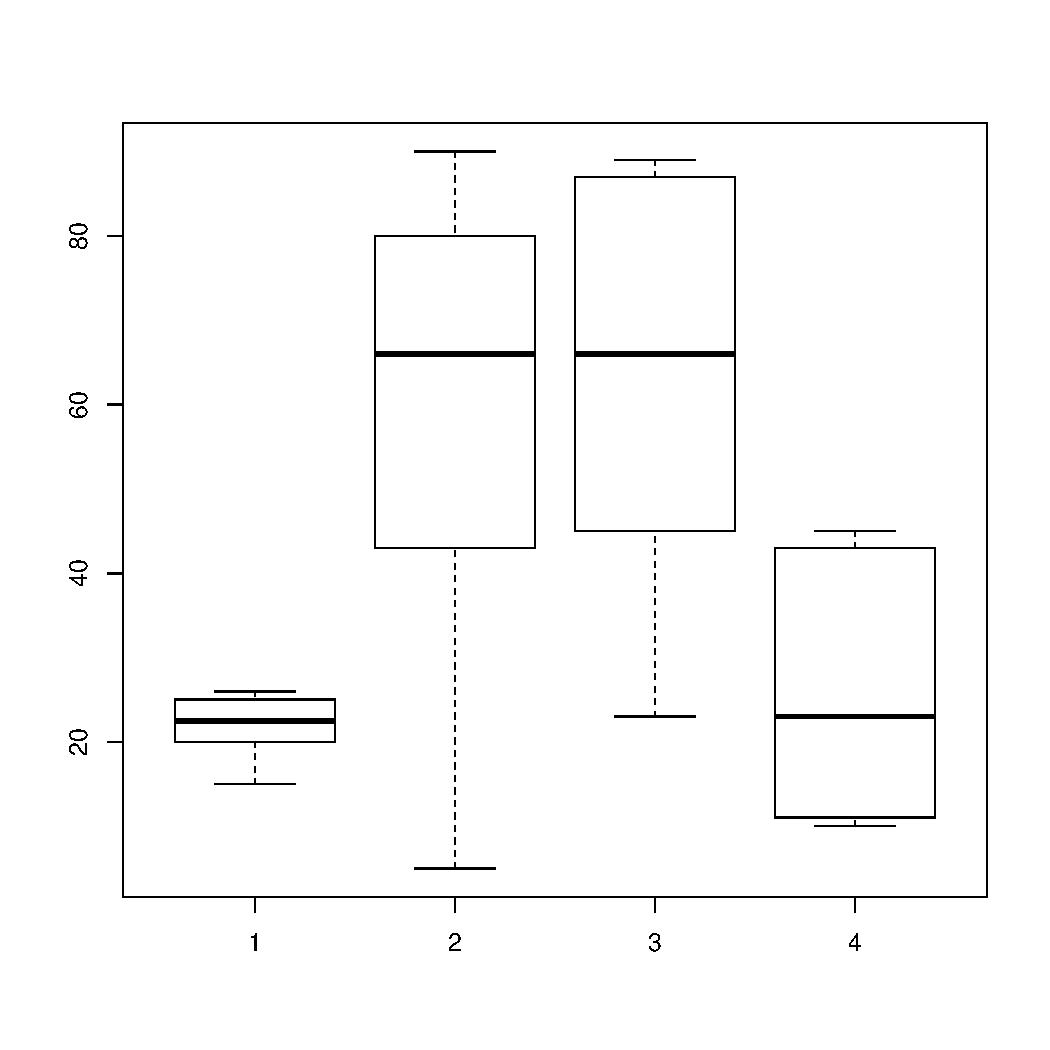
\includegraphics[width=\maxwidth]{figure/unnamed-chunk-147-1} 

\end{knitrout}
\caption{Boxplot comparativo di 4 tipi di grasso di cottura.}
\label{datiist}
\end{center}
\end{figure}
In modo analogo
\begin{knitrout}
\definecolor{shadecolor}{rgb}{0.969, 0.969, 0.969}\color{fgcolor}\begin{kframe}
\begin{alltt}
\hlkwd{anova}\hlstd{(}\hlkwd{lm}\hlstd{(y}\hlopt{~}\hlstd{x))}
\end{alltt}
\begin{verbatim}
## Analysis of Variance Table
## 
## Response: y
##           Df Sum Sq Mean Sq F value   Pr(>F)   
## x          3 8171.0 2723.67  5.8622 0.004833 **
## Residuals 20 9292.3  464.62                    
## ---
## Signif. codes:  
## 0 '***' 0.001 '**' 0.01 '*' 0.05 '.' 0.1 ' ' 1
\end{verbatim}
\end{kframe}
\end{knitrout}

fornisce il risultato dell'analisi della varianza.



\subsection{Test $\chi^2$  di indipendenza}

%code chunk
\begin{knitrout}
\definecolor{shadecolor}{rgb}{0.969, 0.969, 0.969}\color{fgcolor}\begin{kframe}
\begin{alltt}
\hlkwd{read.table}\hlstd{(}\hlstr{"../filedati/PopularKids.html"}\hlstd{,}\hlkwc{skip}\hlstd{=}\hlnum{39}\hlstd{,}\hlkwc{header}\hlstd{=T,}\hlkwc{nrow}\hlstd{=}\hlnum{478}\hlstd{,}\hlkwc{sep}\hlstd{=}\hlstr{"\textbackslash{}t"}\hlstd{)}\hlkwb{->}\hlstd{kidinterest}
\end{alltt}
\end{kframe}
\end{knitrout}
Il test $\chi^2$  di indipendenza consente di  verificare se  due variabili sono indipendenti.
Se consideriamo le due variabili precedenti sesso e interessi.
\textsf{R}  dispone del comando \texttt{chisq.test},\index{\texttt{chisq.tst},test $\chi^2$} dalla sintassi generale:$$\texttt{chisq.test}(\varia{tabella})$$

Nell'esempio
%code chunk
\begin{knitrout}
\definecolor{shadecolor}{rgb}{0.969, 0.969, 0.969}\color{fgcolor}\begin{kframe}
\begin{alltt}
\hlstd{tabellaEH}\hlkwb{=}\hlkwd{table}\hlstd{(studenti}\hlopt{$}\hlstd{Eyes,studenti}\hlopt{$}\hlstd{Hair)}
\hlkwd{chisq.test}\hlstd{(tabellaEH)}
\end{alltt}


{\ttfamily\noindent\color{warningcolor}{\#\# Warning in chisq.test(tabellaEH): Chi-squared approximation may be incorrect}}\begin{verbatim}
## 
## 	Pearson's Chi-squared test
## 
## data:  tabellaEH
## X-squared = 5.9614, df = 4, p-value = 0.202
\end{verbatim}
\end{kframe}
\end{knitrout}
L'intervallo di accettazione dell'ipotesi (che ricordiamo \`e l'indipendenza) al 95\% di fiducia e 1 gradi di libert\`a \`e  $[0, 3.841]$, il consuntivo cade dentro, per cui l'ipotesi \`e accettata.
Per eliminare la correzione di Pearson si utilizza il parametro  \texttt{correct=FALSE}.
Ad esempio scriveremo:
%code chunk
\begin{knitrout}
\definecolor{shadecolor}{rgb}{0.969, 0.969, 0.969}\color{fgcolor}\begin{kframe}
\begin{alltt}
\hlkwd{chisq.test}\hlstd{(tabellaEH,}\hlkwc{correct}\hlstd{=}\hlnum{FALSE}\hlstd{)}
\end{alltt}
\end{kframe}
\end{knitrout}

\subsection{Test $\chi^2$  di adeguamento}
Consideriamo una variabile aleatoria discreta con frequenza assoluta delle uscite racchiuse in una lista \texttt{data}. Ci si pone il problema di stabilire se tali frequenze sono compatibili con le probabilit\`a (riportate nella lista $p$).
\begin{knitrout}
\definecolor{shadecolor}{rgb}{0.969, 0.969, 0.969}\color{fgcolor}\begin{kframe}
\begin{alltt}
\hlstd{data}\hlkwb{<-}\hlkwd{c}\hlstd{(}\hlnum{2}\hlstd{,}\hlnum{3}\hlstd{,}\hlnum{4}\hlstd{,}\hlnum{5}\hlstd{,}\hlnum{6}\hlstd{,}\hlnum{7}\hlstd{,}\hlnum{8}\hlstd{,}\hlnum{9}\hlstd{,}\hlnum{10}\hlstd{,}\hlnum{11}\hlstd{)}
\hlstd{prob}\hlkwb{<-}\hlkwd{c}\hlstd{(}\hlnum{5}\hlstd{,}\hlnum{20}\hlstd{,}\hlnum{5}\hlstd{,}\hlnum{10}\hlstd{,}\hlnum{5}\hlstd{,}\hlnum{15}\hlstd{,}\hlnum{5}\hlstd{,}\hlnum{10}\hlstd{,}\hlnum{10}\hlstd{,}\hlnum{15}\hlstd{)}
\hlkwd{sum}\hlstd{(prob)}
\hlkwd{chisq.test}\hlstd{(data,}\hlkwc{p}\hlstd{=prob,}\hlkwc{rescale.p}\hlstd{=}\hlnum{TRUE}\hlstd{)}
\end{alltt}
\end{kframe}
\end{knitrout}
Si \`e usata qui la scelta \texttt{rescale.p=TRUE} in quanto la somma delle  probabilit\`a non era 1.
L'uscita del test riporta il valore del consuntivo $\chi^2$ i gradi di libert\`a ed il valore $p$.

\section{Distribuzione Binomiale}
Il coefficiente binomiale \`e definito come
\begin{equation*} \texttt{choose}(\varia{n},\varia{m})={n \choose m}=\dfrac{n!}{m!\times (n-m)!}\end{equation*}
Ad esempio
\begin{knitrout}
\definecolor{shadecolor}{rgb}{0.969, 0.969, 0.969}\color{fgcolor}\begin{kframe}
\begin{alltt}
\hlkwd{choose}\hlstd{(}\hlnum{6}\hlstd{,}\hlnum{3}\hlstd{)}
\end{alltt}
\begin{verbatim}
## [1] 20
\end{verbatim}
\end{kframe}
\end{knitrout}
La distribuzione binomiale in \textsf{R} ha la sintassi $$\texttt{dbinom}(\varia{successi},\varia{prove},
\varia{probabilit\`a successo})$$ e fornisce la  probabilit\`a di ottenere nel corso di un certo numero di prove  il numero di successi indicato.\index{\texttt{dbinom}}
Ad esempio, nel lancio di un dado 10 volte, vogliamo determinare la  probabilit\`a che esca  \emph{esattamente} due volte il numero 4:
%codechunk
\begin{knitrout}
\definecolor{shadecolor}{rgb}{0.969, 0.969, 0.969}\color{fgcolor}\begin{kframe}
\begin{alltt}
\hlkwd{dbinom}\hlstd{(}\hlnum{2}\hlstd{,}\hlnum{10}\hlstd{,}\hlnum{1}\hlopt{/}\hlnum{6}\hlstd{)}
\end{alltt}
\begin{verbatim}
## [1] 0.29071
\end{verbatim}
\end{kframe}
\end{knitrout}

La  probabilit\`a \`e circa del 29\%.


\section{Distribuzione di Fisher}

La distribuzione di Fisher \`e indicata in \textsf{R} con la lettera \texttt{f}. Per tracciare il grafico della densit\`a con gradi di libert\`a $\nu_1$ e $\nu_2$ basta scrivere
\begin{knitrout}
\definecolor{shadecolor}{rgb}{0.969, 0.969, 0.969}\color{fgcolor}\begin{kframe}
\begin{alltt}
\hlkwd{curve}\hlstd{(}\hlkwd{df}\hlstd{(x,}\hlnum{3}\hlstd{,}\hlnum{10}\hlstd{),}\hlnum{0}\hlstd{,}\hlnum{5}\hlstd{)}
\end{alltt}
\end{kframe}
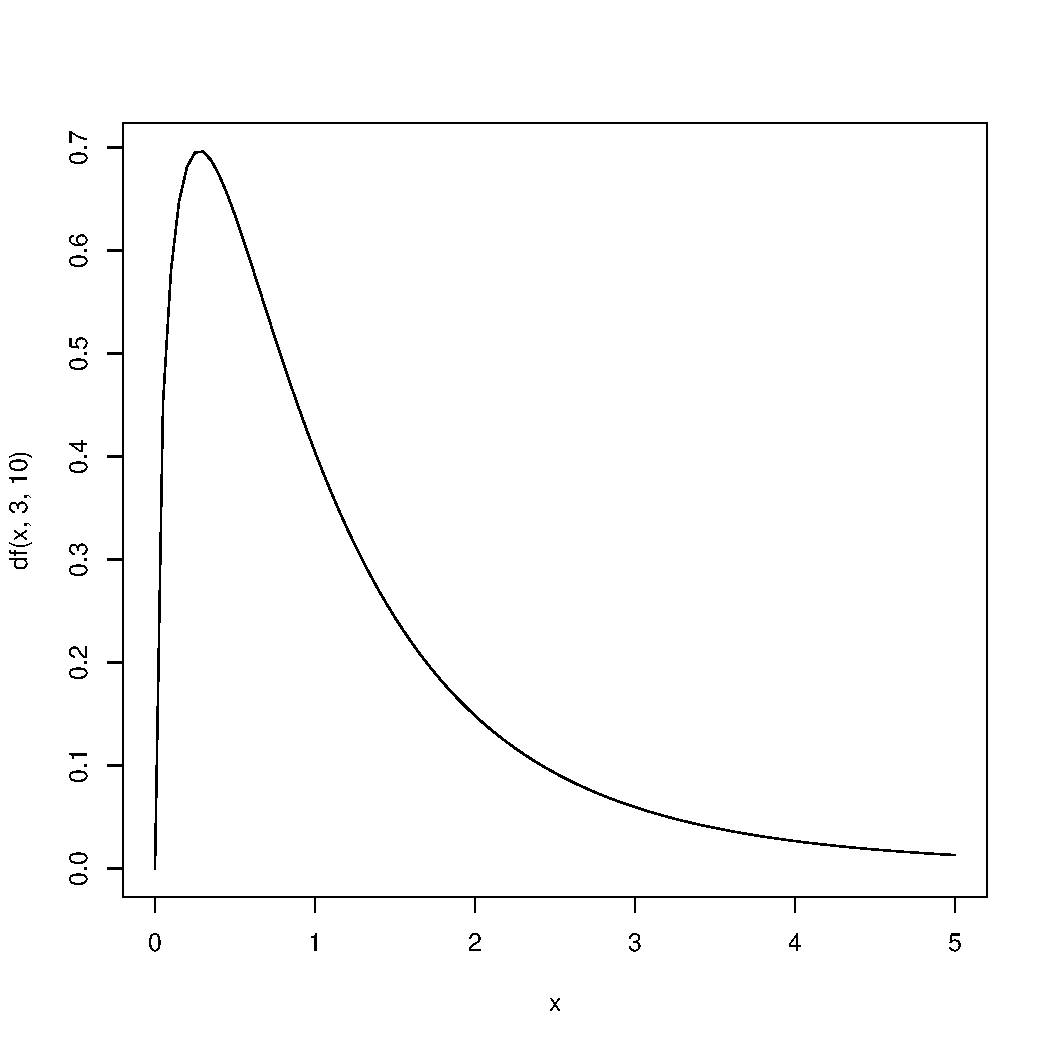
\includegraphics[width=\maxwidth]{figure/unnamed-chunk-155-1} 

\end{knitrout}
ottenendo il grafico
\begin{figure}[htbp]
\begin{center}
\begin{knitrout}
\definecolor{shadecolor}{rgb}{0.969, 0.969, 0.969}\color{fgcolor}\begin{kframe}
\begin{alltt}
\hlkwd{curve}\hlstd{(}\hlkwd{df}\hlstd{(x,}\hlnum{3}\hlstd{,}\hlnum{10}\hlstd{),}\hlnum{0}\hlstd{,}\hlnum{5}\hlstd{)}
\end{alltt}
\end{kframe}
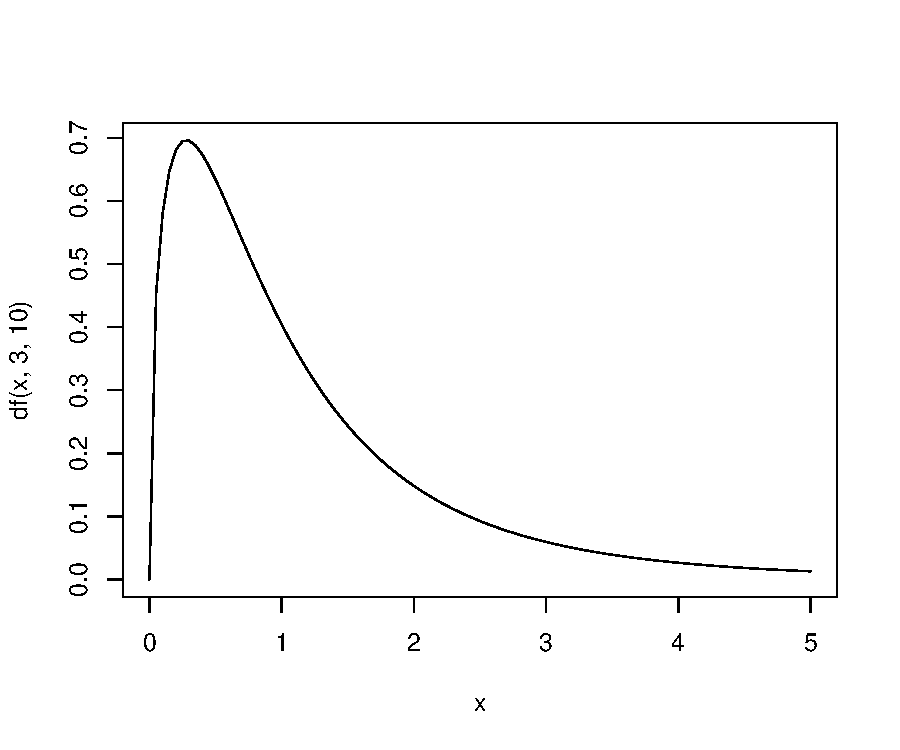
\includegraphics[width=\maxwidth]{figure/unnamed-chunk-156-1} 

\end{knitrout}
\caption{Distribuzione di Fisher.}
\label{fig:fisher}
\end{center}
\end{figure}.

Dobbiamo solo definire $x$, $df1$ e $df2$, gradi di libert\`a per poi applicare \texttt{df},\texttt{qf}, \texttt{rf} come visto per le distribuzioni precedenti.
Per esempio per ottenere il valore della funzione inversa  per $x=0.9$ e $df1=3$ e $df2=4$ scriveremo:
\begin{knitrout}
\definecolor{shadecolor}{rgb}{0.969, 0.969, 0.969}\color{fgcolor}\begin{kframe}
\begin{alltt}
\hlkwd{qf}\hlstd{(}\hlnum{0.9}\hlstd{,}\hlnum{3}\hlstd{,}\hlnum{4}\hlstd{)}
\end{alltt}
\begin{verbatim}
## [1] 4.19086
\end{verbatim}
\end{kframe}
\end{knitrout}


\section{Tabelle di contingenza}

Il comando
$\texttt{table}$ applicato ad un lista contenente valori di una singola variabile nominale conta le frequenze di ciascuna livello, se applicato ad un \emph{dataframe} di $n$  variabili conta le occorrenze di  ciascuna combinazione di livelli possibile ($2^n$ se le variabili sono dicotomiche). Per esempio se consideriamo il \emph{dataframe}  \texttt{studenti}  possiamo creare una tabella dei colori degli occhi e dei capelli
%code chunk
\begin{knitrout}
\definecolor{shadecolor}{rgb}{0.969, 0.969, 0.969}\color{fgcolor}\begin{kframe}
\begin{alltt}
\hlstd{tabellaEH}\hlkwb{=}\hlkwd{table}\hlstd{(studenti}\hlopt{$}\hlstd{Eyes,studenti}\hlopt{$}\hlstd{Hair)}
\end{alltt}
\end{kframe}
\end{knitrout}





 
\vfill\eject
\thispagestyle{empty}\cleardoublepage
 
 


 

